\documentclass[11pt]{article}
\usepackage[utf8]{inputenc}
\usepackage[T1]{fontenc}
\usepackage{textcomp}
\usepackage[a4paper,margin=2.1cm]{geometry}
\usepackage{amsmath,amssymb}
\usepackage{graphicx}
\usepackage{tikz}
\usetikzlibrary{arrows.meta}
\usepackage{xcolor}
\usepackage{mdframed}
\usepackage[colorlinks=true,linkcolor=blue!60!black]{hyperref}
\setlength{\parindent}{0pt}
\setlength{\parskip}{6pt}

\newcommand{\question}[1]{\par\medskip\noindent\textbf{#1}\par}
\newmdenv[linecolor=green!45!black,linewidth=0.8pt,backgroundcolor=green!4,
  innertopmargin=4pt,innerbottommargin=4pt,skipabove=6pt,skipbelow=6pt]{answerbox}

\title{\textbf{Inequalities}\\[0.3em]\large Worked Solutions with TikZ Number-Line Diagrams}
\author{Wisest Maths --- Year 1 A-Level, Solving Linear Inequalities (ref \texttt{ise1})}
\date{}

\begin{document}
\maketitle
\noindent This document contains all 70 \emph{Solving Linear Inequalities} questions, each with a
fully worked solution and a TikZ number-line diagram of the solution set. Open circles denote strict
\(<\)/\(>\) and filled circles denote \(\le\)/\(\ge\); the shaded ray or segment is the solution. For the
\emph{satisfy both} questions the two contributing inequalities are drawn above the axis and their intersection
is shown on the axis.
\tableofcontents
\bigskip
\hrule

\section*{Solving Linear Inequalities 01\quad\small\texttt{(ise1-001)}}
\addcontentsline{toc}{section}{Solving Linear Inequalities 01 (ise1-001)}
\textit{Difficulty: Foundation \quad\textbar\quad Marks: 2}

\question{Find the set of values of \( x \) which satisfy \( 3x - 4 < 11 \).}

\textbf{Worked solution.}

\textit{Step 1: Add 4 to both sides.}
\[\begin{gathered}
3x < 15
\end{gathered}\]
Isolate the term containing \( x \).

\textit{Step 2: Divide both sides by 3.}
\[\begin{gathered}
x < 5
\end{gathered}\]
Dividing by a positive number does not change the direction of the inequality.

\begin{answerbox}
\textbf{Final answer:}\quad \(\displaystyle  x < 5 \)
\end{answerbox}
\textbf{Solution on a number line.}

\begin{center}
\resizebox{\ifdim\width>\linewidth \linewidth\else \width\fi}{!}{%
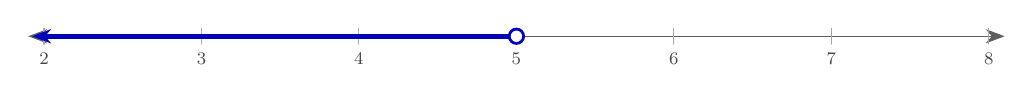
\begin{tikzpicture}[>={Stealth[length=2.4mm]},font=\footnotesize,line cap=round]
\draw[<->,gray!75!black] (-0.2,0) -- (12.2,0);
\draw[gray!70] (0,-0.1) -- (0,0.1);
\node[below,gray!55!black,scale=0.8] at (0,-0.12) {$2$};
\draw[gray!70] (2,-0.1) -- (2,0.1);
\node[below,gray!55!black,scale=0.8] at (2,-0.12) {$3$};
\draw[gray!70] (4,-0.1) -- (4,0.1);
\node[below,gray!55!black,scale=0.8] at (4,-0.12) {$4$};
\draw[gray!70] (6,-0.1) -- (6,0.1);
\node[below,gray!55!black,scale=0.8] at (6,-0.12) {$5$};
\draw[gray!70] (8,-0.1) -- (8,0.1);
\node[below,gray!55!black,scale=0.8] at (8,-0.12) {$6$};
\draw[gray!70] (10,-0.1) -- (10,0.1);
\node[below,gray!55!black,scale=0.8] at (10,-0.12) {$7$};
\draw[gray!70] (12,-0.1) -- (12,0.1);
\node[below,gray!55!black,scale=0.8] at (12,-0.12) {$8$};
\draw[blue!72!black,line width=1.8pt,->] (6,0) -- (-0.15,0);
\draw[blue!72!black,line width=1pt,fill=white] (6,0) circle (2.6pt);
\end{tikzpicture}
}
\end{center}
\medskip\hrule

\section*{Solving Linear Inequalities 02\quad\small\texttt{(ise1-002)}}
\addcontentsline{toc}{section}{Solving Linear Inequalities 02 (ise1-002)}
\textit{Difficulty: Foundation \quad\textbar\quad Marks: 2}

\question{Find the set of values of \( x \) which satisfy \( 2x + 5 \geq 13 \).}

\textbf{Worked solution.}

\textit{Step 1: Subtract 5 from both sides.}
\[\begin{gathered}
2x \geq 8
\end{gathered}\]
Isolate the term containing \( x \).

\textit{Step 2: Divide both sides by 2.}
\[\begin{gathered}
x \geq 4
\end{gathered}\]
Dividing by a positive number keeps the inequality direction unchanged.

\begin{answerbox}
\textbf{Final answer:}\quad \(\displaystyle  x \geq 4 \)
\end{answerbox}
\textbf{Solution on a number line.}

\begin{center}
\resizebox{\ifdim\width>\linewidth \linewidth\else \width\fi}{!}{%
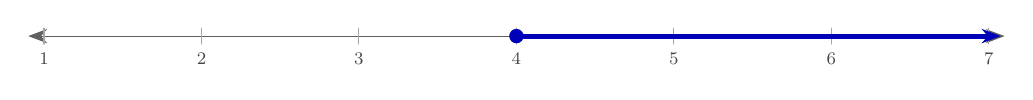
\begin{tikzpicture}[>={Stealth[length=2.4mm]},font=\footnotesize,line cap=round]
\draw[<->,gray!75!black] (-0.2,0) -- (12.2,0);
\draw[gray!70] (0,-0.1) -- (0,0.1);
\node[below,gray!55!black,scale=0.8] at (0,-0.12) {$1$};
\draw[gray!70] (2,-0.1) -- (2,0.1);
\node[below,gray!55!black,scale=0.8] at (2,-0.12) {$2$};
\draw[gray!70] (4,-0.1) -- (4,0.1);
\node[below,gray!55!black,scale=0.8] at (4,-0.12) {$3$};
\draw[gray!70] (6,-0.1) -- (6,0.1);
\node[below,gray!55!black,scale=0.8] at (6,-0.12) {$4$};
\draw[gray!70] (8,-0.1) -- (8,0.1);
\node[below,gray!55!black,scale=0.8] at (8,-0.12) {$5$};
\draw[gray!70] (10,-0.1) -- (10,0.1);
\node[below,gray!55!black,scale=0.8] at (10,-0.12) {$6$};
\draw[gray!70] (12,-0.1) -- (12,0.1);
\node[below,gray!55!black,scale=0.8] at (12,-0.12) {$7$};
\draw[blue!72!black,line width=1.8pt,->] (6,0) -- (12.15,0);
\fill[blue!72!black] (6,0) circle (2.6pt);
\end{tikzpicture}
}
\end{center}
\medskip\hrule

\section*{Solving Linear Inequalities 03\quad\small\texttt{(ise1-003)}}
\addcontentsline{toc}{section}{Solving Linear Inequalities 03 (ise1-003)}
\textit{Difficulty: Foundation \quad\textbar\quad Marks: 2}

\question{Find the set of values of \( x \) which satisfy \( 5x - 3 > 12 \).}

\textbf{Worked solution.}

\textit{Step 1: Add 3 to both sides.}
\[\begin{gathered}
5x > 15
\end{gathered}\]
Isolate the \( x \) term.

\textit{Step 2: Divide both sides by 5.}
\[\begin{gathered}
x > 3
\end{gathered}\]
Positive divisor --- direction unchanged.

\begin{answerbox}
\textbf{Final answer:}\quad \(\displaystyle  x > 3 \)
\end{answerbox}
\textbf{Solution on a number line.}

\begin{center}
\resizebox{\ifdim\width>\linewidth \linewidth\else \width\fi}{!}{%
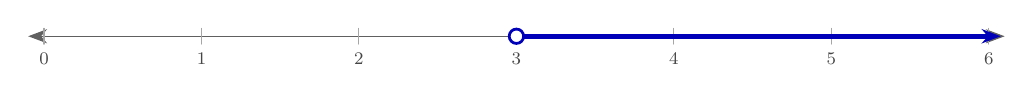
\begin{tikzpicture}[>={Stealth[length=2.4mm]},font=\footnotesize,line cap=round]
\draw[<->,gray!75!black] (-0.2,0) -- (12.2,0);
\draw[gray!70] (0,-0.1) -- (0,0.1);
\node[below,gray!55!black,scale=0.8] at (0,-0.12) {$0$};
\draw[gray!70] (2,-0.1) -- (2,0.1);
\node[below,gray!55!black,scale=0.8] at (2,-0.12) {$1$};
\draw[gray!70] (4,-0.1) -- (4,0.1);
\node[below,gray!55!black,scale=0.8] at (4,-0.12) {$2$};
\draw[gray!70] (6,-0.1) -- (6,0.1);
\node[below,gray!55!black,scale=0.8] at (6,-0.12) {$3$};
\draw[gray!70] (8,-0.1) -- (8,0.1);
\node[below,gray!55!black,scale=0.8] at (8,-0.12) {$4$};
\draw[gray!70] (10,-0.1) -- (10,0.1);
\node[below,gray!55!black,scale=0.8] at (10,-0.12) {$5$};
\draw[gray!70] (12,-0.1) -- (12,0.1);
\node[below,gray!55!black,scale=0.8] at (12,-0.12) {$6$};
\draw[blue!72!black,line width=1.8pt,->] (6,0) -- (12.15,0);
\draw[blue!72!black,line width=1pt,fill=white] (6,0) circle (2.6pt);
\end{tikzpicture}
}
\end{center}
\medskip\hrule

\section*{Solving Linear Inequalities 04\quad\small\texttt{(ise1-004)}}
\addcontentsline{toc}{section}{Solving Linear Inequalities 04 (ise1-004)}
\textit{Difficulty: Foundation \quad\textbar\quad Marks: 2}

\question{Find the set of values of \( x \) which satisfy \( 4x + 7 \leq 3 \).}

\textbf{Worked solution.}

\textit{Step 1: Subtract 7 from both sides.}
\[\begin{gathered}
4x \leq -4
\end{gathered}\]
Isolate the \( x \) term.

\textit{Step 2: Divide both sides by 4.}
\[\begin{gathered}
x \leq -1
\end{gathered}\]
Positive divisor --- direction unchanged.

\begin{answerbox}
\textbf{Final answer:}\quad \(\displaystyle  x \leq -1 \)
\end{answerbox}
\textbf{Solution on a number line.}

\begin{center}
\resizebox{\ifdim\width>\linewidth \linewidth\else \width\fi}{!}{%
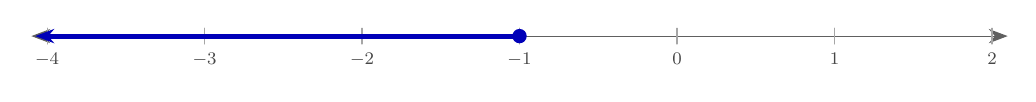
\begin{tikzpicture}[>={Stealth[length=2.4mm]},font=\footnotesize,line cap=round]
\draw[<->,gray!75!black] (-0.2,0) -- (12.2,0);
\draw[gray!70] (0,-0.1) -- (0,0.1);
\node[below,gray!55!black,scale=0.8] at (0,-0.12) {$-4$};
\draw[gray!70] (2,-0.1) -- (2,0.1);
\node[below,gray!55!black,scale=0.8] at (2,-0.12) {$-3$};
\draw[gray!70] (4,-0.1) -- (4,0.1);
\node[below,gray!55!black,scale=0.8] at (4,-0.12) {$-2$};
\draw[gray!70] (6,-0.1) -- (6,0.1);
\node[below,gray!55!black,scale=0.8] at (6,-0.12) {$-1$};
\draw[gray!70] (8,-0.1) -- (8,0.1);
\node[below,gray!55!black,scale=0.8] at (8,-0.12) {$0$};
\draw[gray!70] (10,-0.1) -- (10,0.1);
\node[below,gray!55!black,scale=0.8] at (10,-0.12) {$1$};
\draw[gray!70] (12,-0.1) -- (12,0.1);
\node[below,gray!55!black,scale=0.8] at (12,-0.12) {$2$};
\draw[blue!72!black,line width=1.8pt,->] (6,0) -- (-0.15,0);
\fill[blue!72!black] (6,0) circle (2.6pt);
\end{tikzpicture}
}
\end{center}
\medskip\hrule

\section*{Solving Linear Inequalities 05\quad\small\texttt{(ise1-005)}}
\addcontentsline{toc}{section}{Solving Linear Inequalities 05 (ise1-005)}
\textit{Difficulty: Foundation \quad\textbar\quad Marks: 2}

\question{Find the set of values of \( x \) which satisfy \( 7 - 2x < 1 \).}

\textbf{Worked solution.}

\textit{Step 1: Subtract 7 from both sides.}
\[\begin{gathered}
-2x < -6
\end{gathered}\]
Bring the constant to the right.

\textit{Step 2: Divide both sides by \( -2 \) and reverse the inequality.}
\[\begin{gathered}
x > 3
\end{gathered}\]
Dividing by a negative number reverses the direction of the inequality.

\begin{answerbox}
\textbf{Final answer:}\quad \(\displaystyle  x > 3 \)
\end{answerbox}
\textbf{Solution on a number line.}

\begin{center}
\resizebox{\ifdim\width>\linewidth \linewidth\else \width\fi}{!}{%
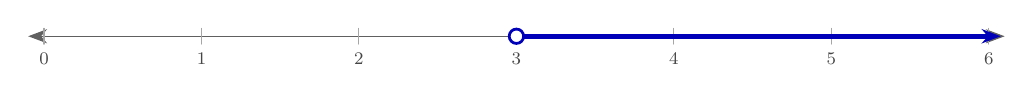
\begin{tikzpicture}[>={Stealth[length=2.4mm]},font=\footnotesize,line cap=round]
\draw[<->,gray!75!black] (-0.2,0) -- (12.2,0);
\draw[gray!70] (0,-0.1) -- (0,0.1);
\node[below,gray!55!black,scale=0.8] at (0,-0.12) {$0$};
\draw[gray!70] (2,-0.1) -- (2,0.1);
\node[below,gray!55!black,scale=0.8] at (2,-0.12) {$1$};
\draw[gray!70] (4,-0.1) -- (4,0.1);
\node[below,gray!55!black,scale=0.8] at (4,-0.12) {$2$};
\draw[gray!70] (6,-0.1) -- (6,0.1);
\node[below,gray!55!black,scale=0.8] at (6,-0.12) {$3$};
\draw[gray!70] (8,-0.1) -- (8,0.1);
\node[below,gray!55!black,scale=0.8] at (8,-0.12) {$4$};
\draw[gray!70] (10,-0.1) -- (10,0.1);
\node[below,gray!55!black,scale=0.8] at (10,-0.12) {$5$};
\draw[gray!70] (12,-0.1) -- (12,0.1);
\node[below,gray!55!black,scale=0.8] at (12,-0.12) {$6$};
\draw[blue!72!black,line width=1.8pt,->] (6,0) -- (12.15,0);
\draw[blue!72!black,line width=1pt,fill=white] (6,0) circle (2.6pt);
\end{tikzpicture}
}
\end{center}
\medskip\hrule

\section*{Solving Linear Inequalities 06\quad\small\texttt{(ise1-006)}}
\addcontentsline{toc}{section}{Solving Linear Inequalities 06 (ise1-006)}
\textit{Difficulty: Foundation \quad\textbar\quad Marks: 2}

\question{Find the set of values of \( x \) which satisfy \( 10 - 3x \geq 1 \).}

\textbf{Worked solution.}

\textit{Step 1: Subtract 10 from both sides.}
\[\begin{gathered}
-3x \geq -9
\end{gathered}\]
Isolate the \( x \) term.

\textit{Step 2: Divide both sides by \( -3 \) and reverse the inequality.}
\[\begin{gathered}
x \leq 3
\end{gathered}\]
Dividing by a negative number flips the inequality.

\begin{answerbox}
\textbf{Final answer:}\quad \(\displaystyle  x \leq 3 \)
\end{answerbox}
\textbf{Solution on a number line.}

\begin{center}
\resizebox{\ifdim\width>\linewidth \linewidth\else \width\fi}{!}{%
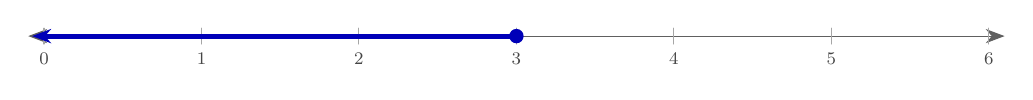
\begin{tikzpicture}[>={Stealth[length=2.4mm]},font=\footnotesize,line cap=round]
\draw[<->,gray!75!black] (-0.2,0) -- (12.2,0);
\draw[gray!70] (0,-0.1) -- (0,0.1);
\node[below,gray!55!black,scale=0.8] at (0,-0.12) {$0$};
\draw[gray!70] (2,-0.1) -- (2,0.1);
\node[below,gray!55!black,scale=0.8] at (2,-0.12) {$1$};
\draw[gray!70] (4,-0.1) -- (4,0.1);
\node[below,gray!55!black,scale=0.8] at (4,-0.12) {$2$};
\draw[gray!70] (6,-0.1) -- (6,0.1);
\node[below,gray!55!black,scale=0.8] at (6,-0.12) {$3$};
\draw[gray!70] (8,-0.1) -- (8,0.1);
\node[below,gray!55!black,scale=0.8] at (8,-0.12) {$4$};
\draw[gray!70] (10,-0.1) -- (10,0.1);
\node[below,gray!55!black,scale=0.8] at (10,-0.12) {$5$};
\draw[gray!70] (12,-0.1) -- (12,0.1);
\node[below,gray!55!black,scale=0.8] at (12,-0.12) {$6$};
\draw[blue!72!black,line width=1.8pt,->] (6,0) -- (-0.15,0);
\fill[blue!72!black] (6,0) circle (2.6pt);
\end{tikzpicture}
}
\end{center}
\medskip\hrule

\section*{Solving Linear Inequalities 07\quad\small\texttt{(ise1-007)}}
\addcontentsline{toc}{section}{Solving Linear Inequalities 07 (ise1-007)}
\textit{Difficulty: Foundation \quad\textbar\quad Marks: 2}

\question{Find the set of values of \( x \) which satisfy \( 8 - 5x > -7 \).}

\textbf{Worked solution.}

\textit{Step 1: Subtract 8 from both sides.}
\[\begin{gathered}
-5x > -15
\end{gathered}\]
Isolate the \( x \) term.

\textit{Step 2: Divide both sides by \( -5 \) and reverse the inequality.}
\[\begin{gathered}
x < 3
\end{gathered}\]
Dividing by a negative reverses the inequality.

\begin{answerbox}
\textbf{Final answer:}\quad \(\displaystyle  x < 3 \)
\end{answerbox}
\textbf{Solution on a number line.}

\begin{center}
\resizebox{\ifdim\width>\linewidth \linewidth\else \width\fi}{!}{%
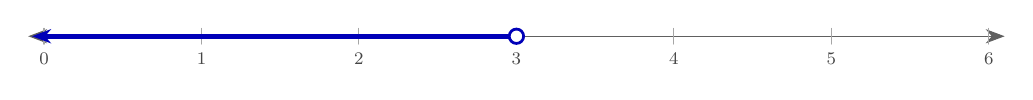
\begin{tikzpicture}[>={Stealth[length=2.4mm]},font=\footnotesize,line cap=round]
\draw[<->,gray!75!black] (-0.2,0) -- (12.2,0);
\draw[gray!70] (0,-0.1) -- (0,0.1);
\node[below,gray!55!black,scale=0.8] at (0,-0.12) {$0$};
\draw[gray!70] (2,-0.1) -- (2,0.1);
\node[below,gray!55!black,scale=0.8] at (2,-0.12) {$1$};
\draw[gray!70] (4,-0.1) -- (4,0.1);
\node[below,gray!55!black,scale=0.8] at (4,-0.12) {$2$};
\draw[gray!70] (6,-0.1) -- (6,0.1);
\node[below,gray!55!black,scale=0.8] at (6,-0.12) {$3$};
\draw[gray!70] (8,-0.1) -- (8,0.1);
\node[below,gray!55!black,scale=0.8] at (8,-0.12) {$4$};
\draw[gray!70] (10,-0.1) -- (10,0.1);
\node[below,gray!55!black,scale=0.8] at (10,-0.12) {$5$};
\draw[gray!70] (12,-0.1) -- (12,0.1);
\node[below,gray!55!black,scale=0.8] at (12,-0.12) {$6$};
\draw[blue!72!black,line width=1.8pt,->] (6,0) -- (-0.15,0);
\draw[blue!72!black,line width=1pt,fill=white] (6,0) circle (2.6pt);
\end{tikzpicture}
}
\end{center}
\medskip\hrule

\section*{Solving Linear Inequalities 08\quad\small\texttt{(ise1-008)}}
\addcontentsline{toc}{section}{Solving Linear Inequalities 08 (ise1-008)}
\textit{Difficulty: Foundation \quad\textbar\quad Marks: 2}

\question{Find the set of values of \( x \) which satisfy \( 12 - 4x \leq 0 \).}

\textbf{Worked solution.}

\textit{Step 1: Subtract 12 from both sides.}
\[\begin{gathered}
-4x \leq -12
\end{gathered}\]
Isolate the \( x \) term.

\textit{Step 2: Divide both sides by \( -4 \) and reverse the inequality.}
\[\begin{gathered}
x \geq 3
\end{gathered}\]
Dividing by a negative flips the inequality.

\begin{answerbox}
\textbf{Final answer:}\quad \(\displaystyle  x \geq 3 \)
\end{answerbox}
\textbf{Solution on a number line.}

\begin{center}
\resizebox{\ifdim\width>\linewidth \linewidth\else \width\fi}{!}{%
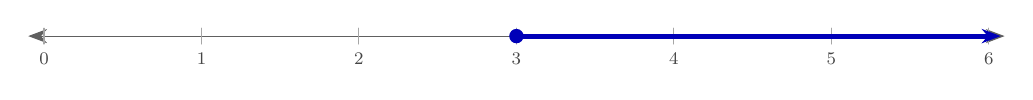
\begin{tikzpicture}[>={Stealth[length=2.4mm]},font=\footnotesize,line cap=round]
\draw[<->,gray!75!black] (-0.2,0) -- (12.2,0);
\draw[gray!70] (0,-0.1) -- (0,0.1);
\node[below,gray!55!black,scale=0.8] at (0,-0.12) {$0$};
\draw[gray!70] (2,-0.1) -- (2,0.1);
\node[below,gray!55!black,scale=0.8] at (2,-0.12) {$1$};
\draw[gray!70] (4,-0.1) -- (4,0.1);
\node[below,gray!55!black,scale=0.8] at (4,-0.12) {$2$};
\draw[gray!70] (6,-0.1) -- (6,0.1);
\node[below,gray!55!black,scale=0.8] at (6,-0.12) {$3$};
\draw[gray!70] (8,-0.1) -- (8,0.1);
\node[below,gray!55!black,scale=0.8] at (8,-0.12) {$4$};
\draw[gray!70] (10,-0.1) -- (10,0.1);
\node[below,gray!55!black,scale=0.8] at (10,-0.12) {$5$};
\draw[gray!70] (12,-0.1) -- (12,0.1);
\node[below,gray!55!black,scale=0.8] at (12,-0.12) {$6$};
\draw[blue!72!black,line width=1.8pt,->] (6,0) -- (12.15,0);
\fill[blue!72!black] (6,0) circle (2.6pt);
\end{tikzpicture}
}
\end{center}
\medskip\hrule

\section*{Solving Linear Inequalities 09\quad\small\texttt{(ise1-009)}}
\addcontentsline{toc}{section}{Solving Linear Inequalities 09 (ise1-009)}
\textit{Difficulty: Foundation \quad\textbar\quad Marks: 2}

\question{Find the set of values of \( x \) which satisfy \( 6x + 1 > 4x + 9 \).}

\textbf{Worked solution.}

\textit{Step 1: Subtract \( 4x \) from both sides.}
\[\begin{gathered}
2x + 1 > 9
\end{gathered}\]
Collect \( x \) terms on the left.

\textit{Step 2: Subtract 1 from both sides.}
\[\begin{gathered}
2x > 8
\end{gathered}\]
Isolate the \( x \) term.

\textit{Step 3: Divide both sides by 2.}
\[\begin{gathered}
x > 4
\end{gathered}\]
Positive divisor --- direction unchanged.

\begin{answerbox}
\textbf{Final answer:}\quad \(\displaystyle  x > 4 \)
\end{answerbox}
\textbf{Solution on a number line.}

\begin{center}
\resizebox{\ifdim\width>\linewidth \linewidth\else \width\fi}{!}{%
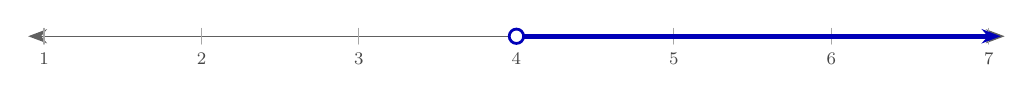
\begin{tikzpicture}[>={Stealth[length=2.4mm]},font=\footnotesize,line cap=round]
\draw[<->,gray!75!black] (-0.2,0) -- (12.2,0);
\draw[gray!70] (0,-0.1) -- (0,0.1);
\node[below,gray!55!black,scale=0.8] at (0,-0.12) {$1$};
\draw[gray!70] (2,-0.1) -- (2,0.1);
\node[below,gray!55!black,scale=0.8] at (2,-0.12) {$2$};
\draw[gray!70] (4,-0.1) -- (4,0.1);
\node[below,gray!55!black,scale=0.8] at (4,-0.12) {$3$};
\draw[gray!70] (6,-0.1) -- (6,0.1);
\node[below,gray!55!black,scale=0.8] at (6,-0.12) {$4$};
\draw[gray!70] (8,-0.1) -- (8,0.1);
\node[below,gray!55!black,scale=0.8] at (8,-0.12) {$5$};
\draw[gray!70] (10,-0.1) -- (10,0.1);
\node[below,gray!55!black,scale=0.8] at (10,-0.12) {$6$};
\draw[gray!70] (12,-0.1) -- (12,0.1);
\node[below,gray!55!black,scale=0.8] at (12,-0.12) {$7$};
\draw[blue!72!black,line width=1.8pt,->] (6,0) -- (12.15,0);
\draw[blue!72!black,line width=1pt,fill=white] (6,0) circle (2.6pt);
\end{tikzpicture}
}
\end{center}
\medskip\hrule

\section*{Solving Linear Inequalities 10\quad\small\texttt{(ise1-010)}}
\addcontentsline{toc}{section}{Solving Linear Inequalities 10 (ise1-010)}
\textit{Difficulty: Foundation \quad\textbar\quad Marks: 2}

\question{Find the set of values of \( x \) which satisfy \( 5x - 2 \leq 3x + 8 \).}

\textbf{Worked solution.}

\textit{Step 1: Subtract \( 3x \) from both sides.}
\[\begin{gathered}
2x - 2 \leq 8
\end{gathered}\]
Collect \( x \) terms on the left.

\textit{Step 2: Add 2 to both sides.}
\[\begin{gathered}
2x \leq 10
\end{gathered}\]
Isolate \( x \).

\textit{Step 3: Divide both sides by 2.}
\[\begin{gathered}
x \leq 5
\end{gathered}\]
Solution found.

\begin{answerbox}
\textbf{Final answer:}\quad \(\displaystyle  x \leq 5 \)
\end{answerbox}
\textbf{Solution on a number line.}

\begin{center}
\resizebox{\ifdim\width>\linewidth \linewidth\else \width\fi}{!}{%
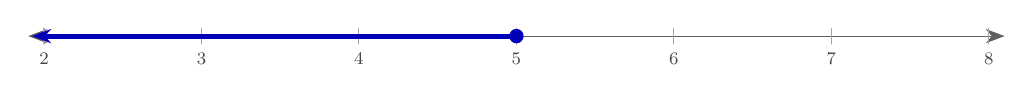
\begin{tikzpicture}[>={Stealth[length=2.4mm]},font=\footnotesize,line cap=round]
\draw[<->,gray!75!black] (-0.2,0) -- (12.2,0);
\draw[gray!70] (0,-0.1) -- (0,0.1);
\node[below,gray!55!black,scale=0.8] at (0,-0.12) {$2$};
\draw[gray!70] (2,-0.1) -- (2,0.1);
\node[below,gray!55!black,scale=0.8] at (2,-0.12) {$3$};
\draw[gray!70] (4,-0.1) -- (4,0.1);
\node[below,gray!55!black,scale=0.8] at (4,-0.12) {$4$};
\draw[gray!70] (6,-0.1) -- (6,0.1);
\node[below,gray!55!black,scale=0.8] at (6,-0.12) {$5$};
\draw[gray!70] (8,-0.1) -- (8,0.1);
\node[below,gray!55!black,scale=0.8] at (8,-0.12) {$6$};
\draw[gray!70] (10,-0.1) -- (10,0.1);
\node[below,gray!55!black,scale=0.8] at (10,-0.12) {$7$};
\draw[gray!70] (12,-0.1) -- (12,0.1);
\node[below,gray!55!black,scale=0.8] at (12,-0.12) {$8$};
\draw[blue!72!black,line width=1.8pt,->] (6,0) -- (-0.15,0);
\fill[blue!72!black] (6,0) circle (2.6pt);
\end{tikzpicture}
}
\end{center}
\medskip\hrule

\section*{Solving Linear Inequalities 11\quad\small\texttt{(ise1-011)}}
\addcontentsline{toc}{section}{Solving Linear Inequalities 11 (ise1-011)}
\textit{Difficulty: Foundation \quad\textbar\quad Marks: 2}

\question{Find the set of values of \( x \) which satisfy \( 7x + 3 < 4x - 6 \).}

\textbf{Worked solution.}

\textit{Step 1: Subtract \( 4x \) from both sides.}
\[\begin{gathered}
3x + 3 < -6
\end{gathered}\]
Collect \( x \) terms on the left.

\textit{Step 2: Subtract 3 from both sides.}
\[\begin{gathered}
3x < -9
\end{gathered}\]
Isolate \( x \).

\textit{Step 3: Divide both sides by 3.}
\[\begin{gathered}
x < -3
\end{gathered}\]
Positive divisor --- direction unchanged.

\begin{answerbox}
\textbf{Final answer:}\quad \(\displaystyle  x < -3 \)
\end{answerbox}
\textbf{Solution on a number line.}

\begin{center}
\resizebox{\ifdim\width>\linewidth \linewidth\else \width\fi}{!}{%
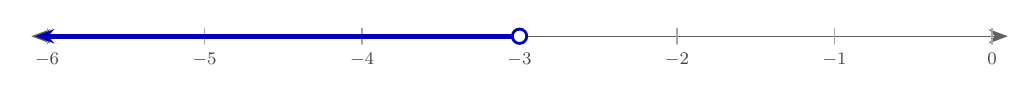
\begin{tikzpicture}[>={Stealth[length=2.4mm]},font=\footnotesize,line cap=round]
\draw[<->,gray!75!black] (-0.2,0) -- (12.2,0);
\draw[gray!70] (0,-0.1) -- (0,0.1);
\node[below,gray!55!black,scale=0.8] at (0,-0.12) {$-6$};
\draw[gray!70] (2,-0.1) -- (2,0.1);
\node[below,gray!55!black,scale=0.8] at (2,-0.12) {$-5$};
\draw[gray!70] (4,-0.1) -- (4,0.1);
\node[below,gray!55!black,scale=0.8] at (4,-0.12) {$-4$};
\draw[gray!70] (6,-0.1) -- (6,0.1);
\node[below,gray!55!black,scale=0.8] at (6,-0.12) {$-3$};
\draw[gray!70] (8,-0.1) -- (8,0.1);
\node[below,gray!55!black,scale=0.8] at (8,-0.12) {$-2$};
\draw[gray!70] (10,-0.1) -- (10,0.1);
\node[below,gray!55!black,scale=0.8] at (10,-0.12) {$-1$};
\draw[gray!70] (12,-0.1) -- (12,0.1);
\node[below,gray!55!black,scale=0.8] at (12,-0.12) {$0$};
\draw[blue!72!black,line width=1.8pt,->] (6,0) -- (-0.15,0);
\draw[blue!72!black,line width=1pt,fill=white] (6,0) circle (2.6pt);
\end{tikzpicture}
}
\end{center}
\medskip\hrule

\section*{Solving Linear Inequalities 12\quad\small\texttt{(ise1-012)}}
\addcontentsline{toc}{section}{Solving Linear Inequalities 12 (ise1-012)}
\textit{Difficulty: Foundation \quad\textbar\quad Marks: 2}

\question{Find the set of values of \( x \) which satisfy \( 9 - x \geq 7x + 1 \).}

\textbf{Worked solution.}

\textit{Step 1: Add \( x \) to both sides.}
\[\begin{gathered}
9 \geq 8x + 1
\end{gathered}\]
Move \( x \) to the right to keep its coefficient positive.

\textit{Step 2: Subtract 1 from both sides.}
\[\begin{gathered}
8 \geq 8x
\end{gathered}\]
Isolate the \( x \) term.

\textit{Step 3: Divide both sides by 8.}
\[\begin{gathered}
1 \geq x \quad \Rightarrow \quad x \leq 1
\end{gathered}\]
Rewrite with \( x \) on the left.

\begin{answerbox}
\textbf{Final answer:}\quad \(\displaystyle  x \leq 1 \)
\end{answerbox}
\textbf{Solution on a number line.}

\begin{center}
\resizebox{\ifdim\width>\linewidth \linewidth\else \width\fi}{!}{%
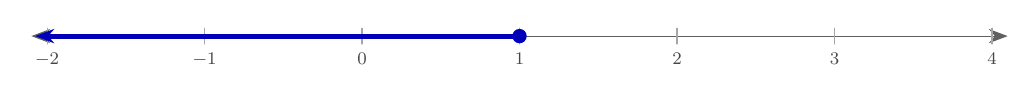
\begin{tikzpicture}[>={Stealth[length=2.4mm]},font=\footnotesize,line cap=round]
\draw[<->,gray!75!black] (-0.2,0) -- (12.2,0);
\draw[gray!70] (0,-0.1) -- (0,0.1);
\node[below,gray!55!black,scale=0.8] at (0,-0.12) {$-2$};
\draw[gray!70] (2,-0.1) -- (2,0.1);
\node[below,gray!55!black,scale=0.8] at (2,-0.12) {$-1$};
\draw[gray!70] (4,-0.1) -- (4,0.1);
\node[below,gray!55!black,scale=0.8] at (4,-0.12) {$0$};
\draw[gray!70] (6,-0.1) -- (6,0.1);
\node[below,gray!55!black,scale=0.8] at (6,-0.12) {$1$};
\draw[gray!70] (8,-0.1) -- (8,0.1);
\node[below,gray!55!black,scale=0.8] at (8,-0.12) {$2$};
\draw[gray!70] (10,-0.1) -- (10,0.1);
\node[below,gray!55!black,scale=0.8] at (10,-0.12) {$3$};
\draw[gray!70] (12,-0.1) -- (12,0.1);
\node[below,gray!55!black,scale=0.8] at (12,-0.12) {$4$};
\draw[blue!72!black,line width=1.8pt,->] (6,0) -- (-0.15,0);
\fill[blue!72!black] (6,0) circle (2.6pt);
\end{tikzpicture}
}
\end{center}
\medskip\hrule

\section*{Solving Linear Inequalities 13\quad\small\texttt{(ise1-013)}}
\addcontentsline{toc}{section}{Solving Linear Inequalities 13 (ise1-013)}
\textit{Difficulty: Foundation \quad\textbar\quad Marks: 2}

\question{Find the set of values of \( x \) which satisfy \( 4 - 3x < 2x - 11 \).}

\textbf{Worked solution.}

\textit{Step 1: Add \( 3x \) to both sides.}
\[\begin{gathered}
4 < 5x - 11
\end{gathered}\]
Eliminate the \( x \) term from the left.

\textit{Step 2: Add 11 to both sides.}
\[\begin{gathered}
15 < 5x
\end{gathered}\]
Isolate \( x \).

\textit{Step 3: Divide both sides by 5.}
\[\begin{gathered}
3 < x \quad \Rightarrow \quad x > 3
\end{gathered}\]
Rewrite with \( x \) on the left.

\begin{answerbox}
\textbf{Final answer:}\quad \(\displaystyle  x > 3 \)
\end{answerbox}
\textbf{Solution on a number line.}

\begin{center}
\resizebox{\ifdim\width>\linewidth \linewidth\else \width\fi}{!}{%
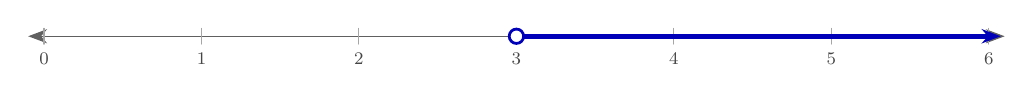
\begin{tikzpicture}[>={Stealth[length=2.4mm]},font=\footnotesize,line cap=round]
\draw[<->,gray!75!black] (-0.2,0) -- (12.2,0);
\draw[gray!70] (0,-0.1) -- (0,0.1);
\node[below,gray!55!black,scale=0.8] at (0,-0.12) {$0$};
\draw[gray!70] (2,-0.1) -- (2,0.1);
\node[below,gray!55!black,scale=0.8] at (2,-0.12) {$1$};
\draw[gray!70] (4,-0.1) -- (4,0.1);
\node[below,gray!55!black,scale=0.8] at (4,-0.12) {$2$};
\draw[gray!70] (6,-0.1) -- (6,0.1);
\node[below,gray!55!black,scale=0.8] at (6,-0.12) {$3$};
\draw[gray!70] (8,-0.1) -- (8,0.1);
\node[below,gray!55!black,scale=0.8] at (8,-0.12) {$4$};
\draw[gray!70] (10,-0.1) -- (10,0.1);
\node[below,gray!55!black,scale=0.8] at (10,-0.12) {$5$};
\draw[gray!70] (12,-0.1) -- (12,0.1);
\node[below,gray!55!black,scale=0.8] at (12,-0.12) {$6$};
\draw[blue!72!black,line width=1.8pt,->] (6,0) -- (12.15,0);
\draw[blue!72!black,line width=1pt,fill=white] (6,0) circle (2.6pt);
\end{tikzpicture}
}
\end{center}
\medskip\hrule

\section*{Solving Linear Inequalities 14\quad\small\texttt{(ise1-014)}}
\addcontentsline{toc}{section}{Solving Linear Inequalities 14 (ise1-014)}
\textit{Difficulty: Foundation \quad\textbar\quad Marks: 2}

\question{Find the set of values of \( x \) which satisfy \( 8x - 1 \geq 5x + 11 \).}

\textbf{Worked solution.}

\textit{Step 1: Subtract \( 5x \) from both sides.}
\[\begin{gathered}
3x - 1 \geq 11
\end{gathered}\]
Collect \( x \) terms on the left.

\textit{Step 2: Add 1 to both sides.}
\[\begin{gathered}
3x \geq 12
\end{gathered}\]
Isolate \( x \).

\textit{Step 3: Divide both sides by 3.}
\[\begin{gathered}
x \geq 4
\end{gathered}\]
Solution found.

\begin{answerbox}
\textbf{Final answer:}\quad \(\displaystyle  x \geq 4 \)
\end{answerbox}
\textbf{Solution on a number line.}

\begin{center}
\resizebox{\ifdim\width>\linewidth \linewidth\else \width\fi}{!}{%
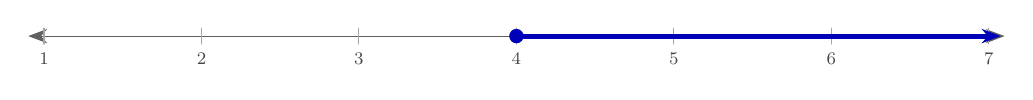
\begin{tikzpicture}[>={Stealth[length=2.4mm]},font=\footnotesize,line cap=round]
\draw[<->,gray!75!black] (-0.2,0) -- (12.2,0);
\draw[gray!70] (0,-0.1) -- (0,0.1);
\node[below,gray!55!black,scale=0.8] at (0,-0.12) {$1$};
\draw[gray!70] (2,-0.1) -- (2,0.1);
\node[below,gray!55!black,scale=0.8] at (2,-0.12) {$2$};
\draw[gray!70] (4,-0.1) -- (4,0.1);
\node[below,gray!55!black,scale=0.8] at (4,-0.12) {$3$};
\draw[gray!70] (6,-0.1) -- (6,0.1);
\node[below,gray!55!black,scale=0.8] at (6,-0.12) {$4$};
\draw[gray!70] (8,-0.1) -- (8,0.1);
\node[below,gray!55!black,scale=0.8] at (8,-0.12) {$5$};
\draw[gray!70] (10,-0.1) -- (10,0.1);
\node[below,gray!55!black,scale=0.8] at (10,-0.12) {$6$};
\draw[gray!70] (12,-0.1) -- (12,0.1);
\node[below,gray!55!black,scale=0.8] at (12,-0.12) {$7$};
\draw[blue!72!black,line width=1.8pt,->] (6,0) -- (12.15,0);
\fill[blue!72!black] (6,0) circle (2.6pt);
\end{tikzpicture}
}
\end{center}
\medskip\hrule

\section*{Solving Linear Inequalities 15\quad\small\texttt{(ise1-015)}}
\addcontentsline{toc}{section}{Solving Linear Inequalities 15 (ise1-015)}
\textit{Difficulty: Foundation \quad\textbar\quad Marks: 2}

\question{Find the set of values of \( x \) which satisfy \( 3 - 4x > 5 - 2x \).}

\textbf{Worked solution.}

\textit{Step 1: Add \( 4x \) to both sides.}
\[\begin{gathered}
3 > 5 + 2x
\end{gathered}\]
Eliminate \( x \) from the left.

\textit{Step 2: Subtract 5 from both sides.}
\[\begin{gathered}
-2 > 2x
\end{gathered}\]
Isolate \( x \).

\textit{Step 3: Divide both sides by 2.}
\[\begin{gathered}
-1 > x \quad \Rightarrow \quad x < -1
\end{gathered}\]
Rewrite with \( x \) on the left.

\begin{answerbox}
\textbf{Final answer:}\quad \(\displaystyle  x < -1 \)
\end{answerbox}
\textbf{Solution on a number line.}

\begin{center}
\resizebox{\ifdim\width>\linewidth \linewidth\else \width\fi}{!}{%
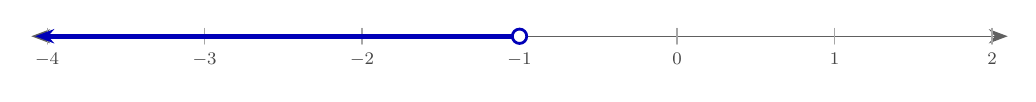
\begin{tikzpicture}[>={Stealth[length=2.4mm]},font=\footnotesize,line cap=round]
\draw[<->,gray!75!black] (-0.2,0) -- (12.2,0);
\draw[gray!70] (0,-0.1) -- (0,0.1);
\node[below,gray!55!black,scale=0.8] at (0,-0.12) {$-4$};
\draw[gray!70] (2,-0.1) -- (2,0.1);
\node[below,gray!55!black,scale=0.8] at (2,-0.12) {$-3$};
\draw[gray!70] (4,-0.1) -- (4,0.1);
\node[below,gray!55!black,scale=0.8] at (4,-0.12) {$-2$};
\draw[gray!70] (6,-0.1) -- (6,0.1);
\node[below,gray!55!black,scale=0.8] at (6,-0.12) {$-1$};
\draw[gray!70] (8,-0.1) -- (8,0.1);
\node[below,gray!55!black,scale=0.8] at (8,-0.12) {$0$};
\draw[gray!70] (10,-0.1) -- (10,0.1);
\node[below,gray!55!black,scale=0.8] at (10,-0.12) {$1$};
\draw[gray!70] (12,-0.1) -- (12,0.1);
\node[below,gray!55!black,scale=0.8] at (12,-0.12) {$2$};
\draw[blue!72!black,line width=1.8pt,->] (6,0) -- (-0.15,0);
\draw[blue!72!black,line width=1pt,fill=white] (6,0) circle (2.6pt);
\end{tikzpicture}
}
\end{center}
\medskip\hrule

\section*{Solving Linear Inequalities 16\quad\small\texttt{(ise1-016)}}
\addcontentsline{toc}{section}{Solving Linear Inequalities 16 (ise1-016)}
\textit{Difficulty: Foundation \quad\textbar\quad Marks: 3}

\question{Find the set of values of \( x \) which satisfy \( 2x - 7 < x + 3 \). Represent the solution on a number line.}

\textbf{Worked solution.}

\textit{Step 1: Subtract \( x \) from both sides.}
\[\begin{gathered}
x - 7 < 3
\end{gathered}\]
Collect \( x \) terms on the left.

\textit{Step 2: Add 7 to both sides.}
\[\begin{gathered}
x < 10
\end{gathered}\]
Isolate \( x \).

\textit{Step 3: On a number line, draw an open circle at 10 and shade to the left.}
\[\begin{gathered}
\longleftarrow \circ\!\!\!\!\!\!10
\end{gathered}\]
Open circle because \( x < 10 \) (10 is not included).

\begin{answerbox}
\textbf{Final answer:}\quad \(\displaystyle  x < 10 \)
\end{answerbox}
\textbf{Solution on a number line.}

\begin{center}
\resizebox{\ifdim\width>\linewidth \linewidth\else \width\fi}{!}{%
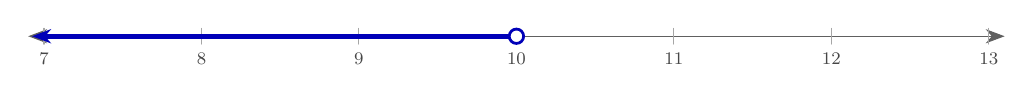
\begin{tikzpicture}[>={Stealth[length=2.4mm]},font=\footnotesize,line cap=round]
\draw[<->,gray!75!black] (-0.2,0) -- (12.2,0);
\draw[gray!70] (0,-0.1) -- (0,0.1);
\node[below,gray!55!black,scale=0.8] at (0,-0.12) {$7$};
\draw[gray!70] (2,-0.1) -- (2,0.1);
\node[below,gray!55!black,scale=0.8] at (2,-0.12) {$8$};
\draw[gray!70] (4,-0.1) -- (4,0.1);
\node[below,gray!55!black,scale=0.8] at (4,-0.12) {$9$};
\draw[gray!70] (6,-0.1) -- (6,0.1);
\node[below,gray!55!black,scale=0.8] at (6,-0.12) {$10$};
\draw[gray!70] (8,-0.1) -- (8,0.1);
\node[below,gray!55!black,scale=0.8] at (8,-0.12) {$11$};
\draw[gray!70] (10,-0.1) -- (10,0.1);
\node[below,gray!55!black,scale=0.8] at (10,-0.12) {$12$};
\draw[gray!70] (12,-0.1) -- (12,0.1);
\node[below,gray!55!black,scale=0.8] at (12,-0.12) {$13$};
\draw[blue!72!black,line width=1.8pt,->] (6,0) -- (-0.15,0);
\draw[blue!72!black,line width=1pt,fill=white] (6,0) circle (2.6pt);
\end{tikzpicture}
}
\end{center}
\medskip\hrule

\section*{Solving Linear Inequalities 17\quad\small\texttt{(ise1-017)}}
\addcontentsline{toc}{section}{Solving Linear Inequalities 17 (ise1-017)}
\textit{Difficulty: Foundation \quad\textbar\quad Marks: 3}

\question{Find the set of values of \( x \) which satisfy \( 4x + 5 > 2x + 13 \). Represent the solution on a number line.}

\textbf{Worked solution.}

\textit{Step 1: Subtract \( 2x \) from both sides.}
\[\begin{gathered}
2x + 5 > 13
\end{gathered}\]
Collect \( x \) terms on the left.

\textit{Step 2: Subtract 5 from both sides.}
\[\begin{gathered}
2x > 8
\end{gathered}\]
Isolate \( x \).

\textit{Step 3: Divide both sides by 2. Show open circle at 4, shading right.}
\[\begin{gathered}
x > 4
\end{gathered}\]
Open circle because 4 is not included.

\begin{answerbox}
\textbf{Final answer:}\quad \(\displaystyle  x > 4 \)
\end{answerbox}
\textbf{Solution on a number line.}

\begin{center}
\resizebox{\ifdim\width>\linewidth \linewidth\else \width\fi}{!}{%
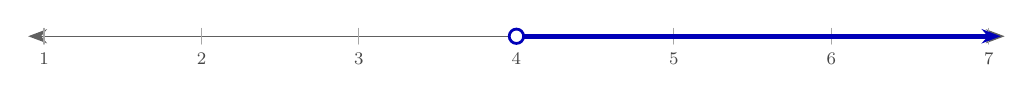
\begin{tikzpicture}[>={Stealth[length=2.4mm]},font=\footnotesize,line cap=round]
\draw[<->,gray!75!black] (-0.2,0) -- (12.2,0);
\draw[gray!70] (0,-0.1) -- (0,0.1);
\node[below,gray!55!black,scale=0.8] at (0,-0.12) {$1$};
\draw[gray!70] (2,-0.1) -- (2,0.1);
\node[below,gray!55!black,scale=0.8] at (2,-0.12) {$2$};
\draw[gray!70] (4,-0.1) -- (4,0.1);
\node[below,gray!55!black,scale=0.8] at (4,-0.12) {$3$};
\draw[gray!70] (6,-0.1) -- (6,0.1);
\node[below,gray!55!black,scale=0.8] at (6,-0.12) {$4$};
\draw[gray!70] (8,-0.1) -- (8,0.1);
\node[below,gray!55!black,scale=0.8] at (8,-0.12) {$5$};
\draw[gray!70] (10,-0.1) -- (10,0.1);
\node[below,gray!55!black,scale=0.8] at (10,-0.12) {$6$};
\draw[gray!70] (12,-0.1) -- (12,0.1);
\node[below,gray!55!black,scale=0.8] at (12,-0.12) {$7$};
\draw[blue!72!black,line width=1.8pt,->] (6,0) -- (12.15,0);
\draw[blue!72!black,line width=1pt,fill=white] (6,0) circle (2.6pt);
\end{tikzpicture}
}
\end{center}
\medskip\hrule

\section*{Solving Linear Inequalities 18\quad\small\texttt{(ise1-018)}}
\addcontentsline{toc}{section}{Solving Linear Inequalities 18 (ise1-018)}
\textit{Difficulty: Foundation \quad\textbar\quad Marks: 3}

\question{Find the set of values of \( x \) which satisfy \( 6x - 3 \geq 3x + 9 \). Represent the solution on a number line.}

\textbf{Worked solution.}

\textit{Step 1: Subtract \( 3x \) from both sides.}
\[\begin{gathered}
3x - 3 \geq 9
\end{gathered}\]
Collect \( x \) terms.

\textit{Step 2: Add 3 to both sides.}
\[\begin{gathered}
3x \geq 12
\end{gathered}\]
Isolate \( x \).

\textit{Step 3: Divide both sides by 3. Show closed circle at 4, shading right.}
\[\begin{gathered}
x \geq 4
\end{gathered}\]
Closed circle because \( x = 4 \) is included.

\begin{answerbox}
\textbf{Final answer:}\quad \(\displaystyle  x \geq 4 \)
\end{answerbox}
\textbf{Solution on a number line.}

\begin{center}
\resizebox{\ifdim\width>\linewidth \linewidth\else \width\fi}{!}{%
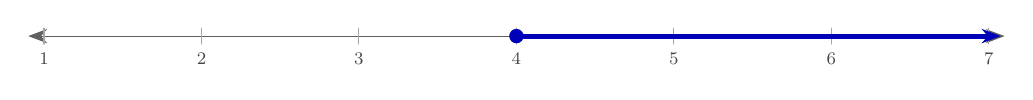
\begin{tikzpicture}[>={Stealth[length=2.4mm]},font=\footnotesize,line cap=round]
\draw[<->,gray!75!black] (-0.2,0) -- (12.2,0);
\draw[gray!70] (0,-0.1) -- (0,0.1);
\node[below,gray!55!black,scale=0.8] at (0,-0.12) {$1$};
\draw[gray!70] (2,-0.1) -- (2,0.1);
\node[below,gray!55!black,scale=0.8] at (2,-0.12) {$2$};
\draw[gray!70] (4,-0.1) -- (4,0.1);
\node[below,gray!55!black,scale=0.8] at (4,-0.12) {$3$};
\draw[gray!70] (6,-0.1) -- (6,0.1);
\node[below,gray!55!black,scale=0.8] at (6,-0.12) {$4$};
\draw[gray!70] (8,-0.1) -- (8,0.1);
\node[below,gray!55!black,scale=0.8] at (8,-0.12) {$5$};
\draw[gray!70] (10,-0.1) -- (10,0.1);
\node[below,gray!55!black,scale=0.8] at (10,-0.12) {$6$};
\draw[gray!70] (12,-0.1) -- (12,0.1);
\node[below,gray!55!black,scale=0.8] at (12,-0.12) {$7$};
\draw[blue!72!black,line width=1.8pt,->] (6,0) -- (12.15,0);
\fill[blue!72!black] (6,0) circle (2.6pt);
\end{tikzpicture}
}
\end{center}
\medskip\hrule

\section*{Solving Linear Inequalities 19\quad\small\texttt{(ise1-019)}}
\addcontentsline{toc}{section}{Solving Linear Inequalities 19 (ise1-019)}
\textit{Difficulty: Foundation \quad\textbar\quad Marks: 3}

\question{Find the set of values of \( x \) which satisfy \( 5x - 4 \leq 2x + 2 \). Represent the solution on a number line.}

\textbf{Worked solution.}

\textit{Step 1: Subtract \( 2x \) from both sides.}
\[\begin{gathered}
3x - 4 \leq 2
\end{gathered}\]
Collect \( x \) terms.

\textit{Step 2: Add 4 to both sides.}
\[\begin{gathered}
3x \leq 6
\end{gathered}\]
Isolate \( x \).

\textit{Step 3: Divide both sides by 3. Show closed circle at 2, shading left.}
\[\begin{gathered}
x \leq 2
\end{gathered}\]
Closed circle because \( x = 2 \) is included.

\begin{answerbox}
\textbf{Final answer:}\quad \(\displaystyle  x \leq 2 \)
\end{answerbox}
\textbf{Solution on a number line.}

\begin{center}
\resizebox{\ifdim\width>\linewidth \linewidth\else \width\fi}{!}{%
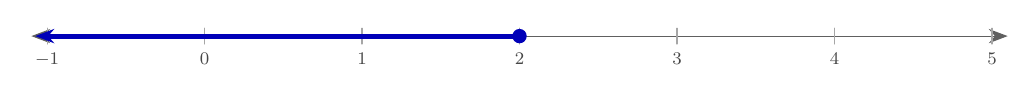
\begin{tikzpicture}[>={Stealth[length=2.4mm]},font=\footnotesize,line cap=round]
\draw[<->,gray!75!black] (-0.2,0) -- (12.2,0);
\draw[gray!70] (0,-0.1) -- (0,0.1);
\node[below,gray!55!black,scale=0.8] at (0,-0.12) {$-1$};
\draw[gray!70] (2,-0.1) -- (2,0.1);
\node[below,gray!55!black,scale=0.8] at (2,-0.12) {$0$};
\draw[gray!70] (4,-0.1) -- (4,0.1);
\node[below,gray!55!black,scale=0.8] at (4,-0.12) {$1$};
\draw[gray!70] (6,-0.1) -- (6,0.1);
\node[below,gray!55!black,scale=0.8] at (6,-0.12) {$2$};
\draw[gray!70] (8,-0.1) -- (8,0.1);
\node[below,gray!55!black,scale=0.8] at (8,-0.12) {$3$};
\draw[gray!70] (10,-0.1) -- (10,0.1);
\node[below,gray!55!black,scale=0.8] at (10,-0.12) {$4$};
\draw[gray!70] (12,-0.1) -- (12,0.1);
\node[below,gray!55!black,scale=0.8] at (12,-0.12) {$5$};
\draw[blue!72!black,line width=1.8pt,->] (6,0) -- (-0.15,0);
\fill[blue!72!black] (6,0) circle (2.6pt);
\end{tikzpicture}
}
\end{center}
\medskip\hrule

\section*{Solving Linear Inequalities 20\quad\small\texttt{(ise1-020)}}
\addcontentsline{toc}{section}{Solving Linear Inequalities 20 (ise1-020)}
\textit{Difficulty: Foundation \quad\textbar\quad Marks: 3}

\question{Find the set of values of \( x \) which satisfy \( 11 - 3x < 5 - x \). Represent the solution on a number line.}

\textbf{Worked solution.}

\textit{Step 1: Add \( 3x \) to both sides.}
\[\begin{gathered}
11 < 5 + 2x
\end{gathered}\]
Eliminate \( x \) from the left.

\textit{Step 2: Subtract 5 from both sides.}
\[\begin{gathered}
6 < 2x
\end{gathered}\]
Isolate \( x \).

\textit{Step 3: Divide both sides by 2. Show open circle at 3, shading right.}
\[\begin{gathered}
3 < x \quad \Rightarrow \quad x > 3
\end{gathered}\]
Open circle at 3.

\begin{answerbox}
\textbf{Final answer:}\quad \(\displaystyle  x > 3 \)
\end{answerbox}
\textbf{Solution on a number line.}

\begin{center}
\resizebox{\ifdim\width>\linewidth \linewidth\else \width\fi}{!}{%
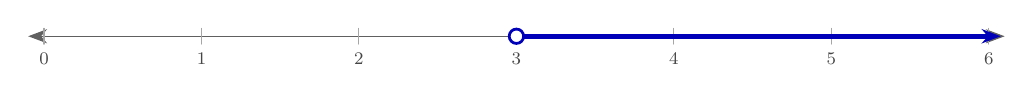
\begin{tikzpicture}[>={Stealth[length=2.4mm]},font=\footnotesize,line cap=round]
\draw[<->,gray!75!black] (-0.2,0) -- (12.2,0);
\draw[gray!70] (0,-0.1) -- (0,0.1);
\node[below,gray!55!black,scale=0.8] at (0,-0.12) {$0$};
\draw[gray!70] (2,-0.1) -- (2,0.1);
\node[below,gray!55!black,scale=0.8] at (2,-0.12) {$1$};
\draw[gray!70] (4,-0.1) -- (4,0.1);
\node[below,gray!55!black,scale=0.8] at (4,-0.12) {$2$};
\draw[gray!70] (6,-0.1) -- (6,0.1);
\node[below,gray!55!black,scale=0.8] at (6,-0.12) {$3$};
\draw[gray!70] (8,-0.1) -- (8,0.1);
\node[below,gray!55!black,scale=0.8] at (8,-0.12) {$4$};
\draw[gray!70] (10,-0.1) -- (10,0.1);
\node[below,gray!55!black,scale=0.8] at (10,-0.12) {$5$};
\draw[gray!70] (12,-0.1) -- (12,0.1);
\node[below,gray!55!black,scale=0.8] at (12,-0.12) {$6$};
\draw[blue!72!black,line width=1.8pt,->] (6,0) -- (12.15,0);
\draw[blue!72!black,line width=1pt,fill=white] (6,0) circle (2.6pt);
\end{tikzpicture}
}
\end{center}
\medskip\hrule

\section*{Solving Linear Inequalities 21\quad\small\texttt{(ise1-021)}}
\addcontentsline{toc}{section}{Solving Linear Inequalities 21 (ise1-021)}
\textit{Difficulty: Foundation \quad\textbar\quad Marks: 2}

\question{Find the set of values of \( x \) which satisfy \( 14 - 2x > 6 + 2x \).}

\textbf{Worked solution.}

\textit{Step 1: Add \( 2x \) to both sides.}
\[\begin{gathered}
14 > 6 + 4x
\end{gathered}\]
Eliminate \( x \) from the left.

\textit{Step 2: Subtract 6 from both sides.}
\[\begin{gathered}
8 > 4x
\end{gathered}\]
Isolate \( x \).

\textit{Step 3: Divide by 4.}
\[\begin{gathered}
2 > x \quad \Rightarrow \quad x < 2
\end{gathered}\]
Positive divisor --- direction unchanged.

\begin{answerbox}
\textbf{Final answer:}\quad \(\displaystyle  x < 2 \)
\end{answerbox}
\textbf{Solution on a number line.}

\begin{center}
\resizebox{\ifdim\width>\linewidth \linewidth\else \width\fi}{!}{%
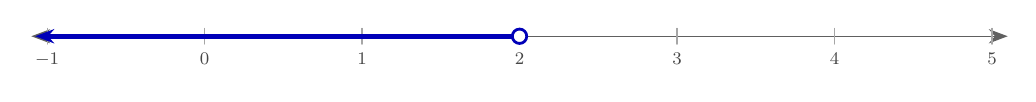
\begin{tikzpicture}[>={Stealth[length=2.4mm]},font=\footnotesize,line cap=round]
\draw[<->,gray!75!black] (-0.2,0) -- (12.2,0);
\draw[gray!70] (0,-0.1) -- (0,0.1);
\node[below,gray!55!black,scale=0.8] at (0,-0.12) {$-1$};
\draw[gray!70] (2,-0.1) -- (2,0.1);
\node[below,gray!55!black,scale=0.8] at (2,-0.12) {$0$};
\draw[gray!70] (4,-0.1) -- (4,0.1);
\node[below,gray!55!black,scale=0.8] at (4,-0.12) {$1$};
\draw[gray!70] (6,-0.1) -- (6,0.1);
\node[below,gray!55!black,scale=0.8] at (6,-0.12) {$2$};
\draw[gray!70] (8,-0.1) -- (8,0.1);
\node[below,gray!55!black,scale=0.8] at (8,-0.12) {$3$};
\draw[gray!70] (10,-0.1) -- (10,0.1);
\node[below,gray!55!black,scale=0.8] at (10,-0.12) {$4$};
\draw[gray!70] (12,-0.1) -- (12,0.1);
\node[below,gray!55!black,scale=0.8] at (12,-0.12) {$5$};
\draw[blue!72!black,line width=1.8pt,->] (6,0) -- (-0.15,0);
\draw[blue!72!black,line width=1pt,fill=white] (6,0) circle (2.6pt);
\end{tikzpicture}
}
\end{center}
\medskip\hrule

\section*{Solving Linear Inequalities 22\quad\small\texttt{(ise1-022)}}
\addcontentsline{toc}{section}{Solving Linear Inequalities 22 (ise1-022)}
\textit{Difficulty: Foundation \quad\textbar\quad Marks: 2}

\question{Find the set of values of \( x \) which satisfy \( 9x - 4 < 6x + 2 \).}

\textbf{Worked solution.}

\textit{Step 1: Subtract \( 6x \) from both sides.}
\[\begin{gathered}
3x - 4 < 2
\end{gathered}\]
Collect \( x \) terms on the left.

\textit{Step 2: Add 4 to both sides.}
\[\begin{gathered}
3x < 6
\end{gathered}\]
Isolate \( x \).

\textit{Step 3: Divide by 3.}
\[\begin{gathered}
x < 2
\end{gathered}\]
Solution found.

\begin{answerbox}
\textbf{Final answer:}\quad \(\displaystyle  x < 2 \)
\end{answerbox}
\textbf{Solution on a number line.}

\begin{center}
\resizebox{\ifdim\width>\linewidth \linewidth\else \width\fi}{!}{%
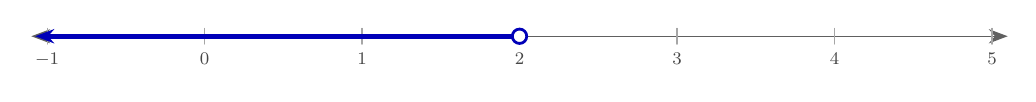
\begin{tikzpicture}[>={Stealth[length=2.4mm]},font=\footnotesize,line cap=round]
\draw[<->,gray!75!black] (-0.2,0) -- (12.2,0);
\draw[gray!70] (0,-0.1) -- (0,0.1);
\node[below,gray!55!black,scale=0.8] at (0,-0.12) {$-1$};
\draw[gray!70] (2,-0.1) -- (2,0.1);
\node[below,gray!55!black,scale=0.8] at (2,-0.12) {$0$};
\draw[gray!70] (4,-0.1) -- (4,0.1);
\node[below,gray!55!black,scale=0.8] at (4,-0.12) {$1$};
\draw[gray!70] (6,-0.1) -- (6,0.1);
\node[below,gray!55!black,scale=0.8] at (6,-0.12) {$2$};
\draw[gray!70] (8,-0.1) -- (8,0.1);
\node[below,gray!55!black,scale=0.8] at (8,-0.12) {$3$};
\draw[gray!70] (10,-0.1) -- (10,0.1);
\node[below,gray!55!black,scale=0.8] at (10,-0.12) {$4$};
\draw[gray!70] (12,-0.1) -- (12,0.1);
\node[below,gray!55!black,scale=0.8] at (12,-0.12) {$5$};
\draw[blue!72!black,line width=1.8pt,->] (6,0) -- (-0.15,0);
\draw[blue!72!black,line width=1pt,fill=white] (6,0) circle (2.6pt);
\end{tikzpicture}
}
\end{center}
\medskip\hrule

\section*{Solving Linear Inequalities 23\quad\small\texttt{(ise1-023)}}
\addcontentsline{toc}{section}{Solving Linear Inequalities 23 (ise1-023)}
\textit{Difficulty: Foundation \quad\textbar\quad Marks: 2}

\question{Find the set of values of \( x \) which satisfy \( 7x + 2 \leq 4x - 7 \).}

\textbf{Worked solution.}

\textit{Step 1: Subtract \( 4x \) from both sides.}
\[\begin{gathered}
3x + 2 \leq -7
\end{gathered}\]
Collect \( x \) terms.

\textit{Step 2: Subtract 2 from both sides.}
\[\begin{gathered}
3x \leq -9
\end{gathered}\]
Isolate \( x \).

\textit{Step 3: Divide by 3.}
\[\begin{gathered}
x \leq -3
\end{gathered}\]
Positive divisor --- direction unchanged.

\begin{answerbox}
\textbf{Final answer:}\quad \(\displaystyle  x \leq -3 \)
\end{answerbox}
\textbf{Solution on a number line.}

\begin{center}
\resizebox{\ifdim\width>\linewidth \linewidth\else \width\fi}{!}{%
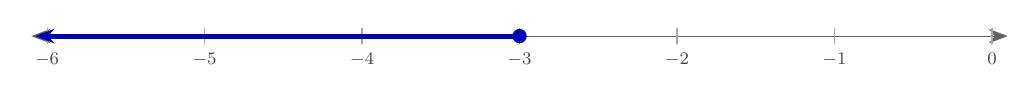
\begin{tikzpicture}[>={Stealth[length=2.4mm]},font=\footnotesize,line cap=round]
\draw[<->,gray!75!black] (-0.2,0) -- (12.2,0);
\draw[gray!70] (0,-0.1) -- (0,0.1);
\node[below,gray!55!black,scale=0.8] at (0,-0.12) {$-6$};
\draw[gray!70] (2,-0.1) -- (2,0.1);
\node[below,gray!55!black,scale=0.8] at (2,-0.12) {$-5$};
\draw[gray!70] (4,-0.1) -- (4,0.1);
\node[below,gray!55!black,scale=0.8] at (4,-0.12) {$-4$};
\draw[gray!70] (6,-0.1) -- (6,0.1);
\node[below,gray!55!black,scale=0.8] at (6,-0.12) {$-3$};
\draw[gray!70] (8,-0.1) -- (8,0.1);
\node[below,gray!55!black,scale=0.8] at (8,-0.12) {$-2$};
\draw[gray!70] (10,-0.1) -- (10,0.1);
\node[below,gray!55!black,scale=0.8] at (10,-0.12) {$-1$};
\draw[gray!70] (12,-0.1) -- (12,0.1);
\node[below,gray!55!black,scale=0.8] at (12,-0.12) {$0$};
\draw[blue!72!black,line width=1.8pt,->] (6,0) -- (-0.15,0);
\fill[blue!72!black] (6,0) circle (2.6pt);
\end{tikzpicture}
}
\end{center}
\medskip\hrule

\section*{Solving Linear Inequalities 24\quad\small\texttt{(ise1-024)}}
\addcontentsline{toc}{section}{Solving Linear Inequalities 24 (ise1-024)}
\textit{Difficulty: Foundation \quad\textbar\quad Marks: 3}

\question{Find the set of values of \( x \) which satisfy \( 12x - 9 \leq 4x + 11 \). Give your answer in set notation.}

\textbf{Worked solution.}

\textit{Step 1: Subtract \( 4x \) from both sides.}
\[\begin{gathered}
8x - 9 \leq 11
\end{gathered}\]
Collect \( x \) terms.

\textit{Step 2: Add 9 to both sides.}
\[\begin{gathered}
8x \leq 20
\end{gathered}\]
Isolate \( x \).

\textit{Step 3: Divide by 8.}
\[\begin{gathered}
x \leq \dfrac{5}{2}
\end{gathered}\]
\( 20 \div 8 = \dfrac{5}{2} \).

\textit{Step 4: Write in set notation.}
\[\begin{gathered}
\{x : x \leq \tfrac{5}{2}\}
\end{gathered}\]
Use curly brackets and a colon for set notation.

\begin{answerbox}
\textbf{Final answer:}\quad \(\displaystyle  \{x : x \leq \tfrac{5}{2}\} \)
\end{answerbox}
\textbf{Solution on a number line.}

\begin{center}
\resizebox{\ifdim\width>\linewidth \linewidth\else \width\fi}{!}{%
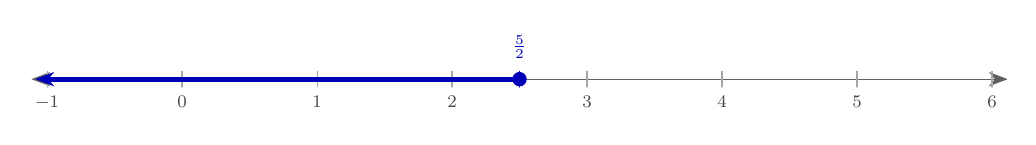
\begin{tikzpicture}[>={Stealth[length=2.4mm]},font=\footnotesize,line cap=round]
\draw[<->,gray!75!black] (-0.2,0) -- (12.2,0);
\draw[gray!70] (0,-0.1) -- (0,0.1);
\node[below,gray!55!black,scale=0.8] at (0,-0.12) {$-1$};
\draw[gray!70] (1.714,-0.1) -- (1.714,0.1);
\node[below,gray!55!black,scale=0.8] at (1.714,-0.12) {$0$};
\draw[gray!70] (3.429,-0.1) -- (3.429,0.1);
\node[below,gray!55!black,scale=0.8] at (3.429,-0.12) {$1$};
\draw[gray!70] (5.143,-0.1) -- (5.143,0.1);
\node[below,gray!55!black,scale=0.8] at (5.143,-0.12) {$2$};
\draw[gray!70] (6.857,-0.1) -- (6.857,0.1);
\node[below,gray!55!black,scale=0.8] at (6.857,-0.12) {$3$};
\draw[gray!70] (8.571,-0.1) -- (8.571,0.1);
\node[below,gray!55!black,scale=0.8] at (8.571,-0.12) {$4$};
\draw[gray!70] (10.286,-0.1) -- (10.286,0.1);
\node[below,gray!55!black,scale=0.8] at (10.286,-0.12) {$5$};
\draw[gray!70] (12,-0.1) -- (12,0.1);
\node[below,gray!55!black,scale=0.8] at (12,-0.12) {$6$};
\draw[blue!72!black,line width=1.8pt,->] (6,0) -- (-0.15,0);
\fill[blue!72!black] (6,0) circle (2.6pt);
\draw[blue!72!black] (6,-0.1) -- (6,0.1);
\node[above,blue!72!black,scale=0.82] at (6,0.16) {$\frac{5}{2}$};
\end{tikzpicture}
}
\end{center}
\medskip\hrule

\section*{Solving Linear Inequalities 25\quad\small\texttt{(ise1-025)}}
\addcontentsline{toc}{section}{Solving Linear Inequalities 25 (ise1-025)}
\textit{Difficulty: Foundation \quad\textbar\quad Marks: 3}

\question{Find the set of values of \( x \) which satisfy \( 5x + 8 > 3 - 2x \). Give your answer in set notation.}

\textbf{Worked solution.}

\textit{Step 1: Add \( 2x \) to both sides.}
\[\begin{gathered}
7x + 8 > 3
\end{gathered}\]
Collect \( x \) terms.

\textit{Step 2: Subtract 8 from both sides.}
\[\begin{gathered}
7x > -5
\end{gathered}\]
Isolate \( x \).

\textit{Step 3: Divide by 7 and write in set notation.}
\[\begin{gathered}
x > -\dfrac{5}{7} \quad \Rightarrow \quad \{x : x > -\tfrac{5}{7}\}
\end{gathered}\]
Positive divisor --- direction unchanged.

\begin{answerbox}
\textbf{Final answer:}\quad \(\displaystyle  \{x : x > -\tfrac{5}{7}\} \)
\end{answerbox}
\textbf{Solution on a number line.}

\begin{center}
\resizebox{\ifdim\width>\linewidth \linewidth\else \width\fi}{!}{%
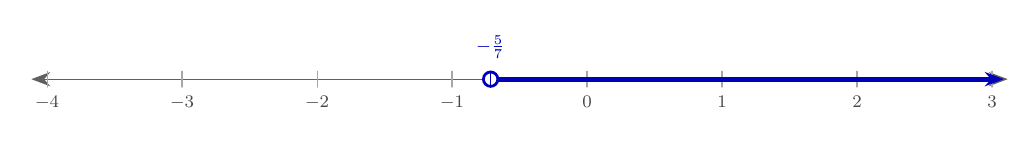
\begin{tikzpicture}[>={Stealth[length=2.4mm]},font=\footnotesize,line cap=round]
\draw[<->,gray!75!black] (-0.2,0) -- (12.2,0);
\draw[gray!70] (0,-0.1) -- (0,0.1);
\node[below,gray!55!black,scale=0.8] at (0,-0.12) {$-4$};
\draw[gray!70] (1.714,-0.1) -- (1.714,0.1);
\node[below,gray!55!black,scale=0.8] at (1.714,-0.12) {$-3$};
\draw[gray!70] (3.429,-0.1) -- (3.429,0.1);
\node[below,gray!55!black,scale=0.8] at (3.429,-0.12) {$-2$};
\draw[gray!70] (5.143,-0.1) -- (5.143,0.1);
\node[below,gray!55!black,scale=0.8] at (5.143,-0.12) {$-1$};
\draw[gray!70] (6.857,-0.1) -- (6.857,0.1);
\node[below,gray!55!black,scale=0.8] at (6.857,-0.12) {$0$};
\draw[gray!70] (8.571,-0.1) -- (8.571,0.1);
\node[below,gray!55!black,scale=0.8] at (8.571,-0.12) {$1$};
\draw[gray!70] (10.286,-0.1) -- (10.286,0.1);
\node[below,gray!55!black,scale=0.8] at (10.286,-0.12) {$2$};
\draw[gray!70] (12,-0.1) -- (12,0.1);
\node[below,gray!55!black,scale=0.8] at (12,-0.12) {$3$};
\draw[blue!72!black,line width=1.8pt,->] (5.633,0) -- (12.15,0);
\draw[blue!72!black,line width=1pt,fill=white] (5.633,0) circle (2.6pt);
\draw[blue!72!black] (5.633,-0.1) -- (5.633,0.1);
\node[above,blue!72!black,scale=0.82] at (5.633,0.16) {$-\frac{5}{7}$};
\end{tikzpicture}
}
\end{center}
\medskip\hrule

\section*{Solving Linear Inequalities 26\quad\small\texttt{(ise1-026)}}
\addcontentsline{toc}{section}{Solving Linear Inequalities 26 (ise1-026)}
\textit{Difficulty: Foundation \quad\textbar\quad Marks: 3}

\question{Find the set of values of \( x \) which satisfy \( 3(x + 4) > 2(x + 7) \).}

\textbf{Worked solution.}

\textit{Step 1: Expand both brackets.}
\[\begin{gathered}
3x + 12 > 2x + 14
\end{gathered}\]
\( 3 \times (x + 4) = 3x + 12 \) and \( 2 \times (x + 7) = 2x + 14 \).

\textit{Step 2: Subtract \( 2x \) from both sides.}
\[\begin{gathered}
x + 12 > 14
\end{gathered}\]
Collect \( x \) terms.

\textit{Step 3: Subtract 12 from both sides.}
\[\begin{gathered}
x > 2
\end{gathered}\]
Solution found.

\begin{answerbox}
\textbf{Final answer:}\quad \(\displaystyle  x > 2 \)
\end{answerbox}
\textbf{Solution on a number line.}

\begin{center}
\resizebox{\ifdim\width>\linewidth \linewidth\else \width\fi}{!}{%
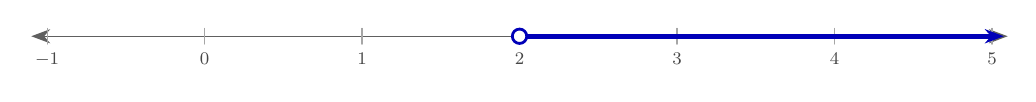
\begin{tikzpicture}[>={Stealth[length=2.4mm]},font=\footnotesize,line cap=round]
\draw[<->,gray!75!black] (-0.2,0) -- (12.2,0);
\draw[gray!70] (0,-0.1) -- (0,0.1);
\node[below,gray!55!black,scale=0.8] at (0,-0.12) {$-1$};
\draw[gray!70] (2,-0.1) -- (2,0.1);
\node[below,gray!55!black,scale=0.8] at (2,-0.12) {$0$};
\draw[gray!70] (4,-0.1) -- (4,0.1);
\node[below,gray!55!black,scale=0.8] at (4,-0.12) {$1$};
\draw[gray!70] (6,-0.1) -- (6,0.1);
\node[below,gray!55!black,scale=0.8] at (6,-0.12) {$2$};
\draw[gray!70] (8,-0.1) -- (8,0.1);
\node[below,gray!55!black,scale=0.8] at (8,-0.12) {$3$};
\draw[gray!70] (10,-0.1) -- (10,0.1);
\node[below,gray!55!black,scale=0.8] at (10,-0.12) {$4$};
\draw[gray!70] (12,-0.1) -- (12,0.1);
\node[below,gray!55!black,scale=0.8] at (12,-0.12) {$5$};
\draw[blue!72!black,line width=1.8pt,->] (6,0) -- (12.15,0);
\draw[blue!72!black,line width=1pt,fill=white] (6,0) circle (2.6pt);
\end{tikzpicture}
}
\end{center}
\medskip\hrule

\section*{Solving Linear Inequalities 27\quad\small\texttt{(ise1-027)}}
\addcontentsline{toc}{section}{Solving Linear Inequalities 27 (ise1-027)}
\textit{Difficulty: Foundation \quad\textbar\quad Marks: 3}

\question{Find the set of values of \( x \) which satisfy \( 4(x - 1) \leq 3(x + 2) \).}

\textbf{Worked solution.}

\textit{Step 1: Expand both brackets.}
\[\begin{gathered}
4x - 4 \leq 3x + 6
\end{gathered}\]
\( 4(x-1) = 4x - 4 \) and \( 3(x+2) = 3x + 6 \).

\textit{Step 2: Subtract \( 3x \) from both sides.}
\[\begin{gathered}
x - 4 \leq 6
\end{gathered}\]
Collect \( x \) terms.

\textit{Step 3: Add 4 to both sides.}
\[\begin{gathered}
x \leq 10
\end{gathered}\]
Solution found.

\begin{answerbox}
\textbf{Final answer:}\quad \(\displaystyle  x \leq 10 \)
\end{answerbox}
\textbf{Solution on a number line.}

\begin{center}
\resizebox{\ifdim\width>\linewidth \linewidth\else \width\fi}{!}{%
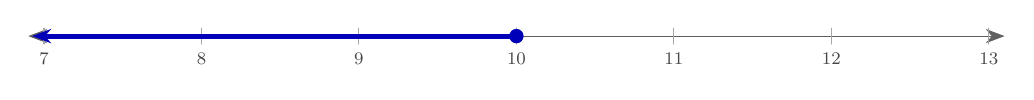
\begin{tikzpicture}[>={Stealth[length=2.4mm]},font=\footnotesize,line cap=round]
\draw[<->,gray!75!black] (-0.2,0) -- (12.2,0);
\draw[gray!70] (0,-0.1) -- (0,0.1);
\node[below,gray!55!black,scale=0.8] at (0,-0.12) {$7$};
\draw[gray!70] (2,-0.1) -- (2,0.1);
\node[below,gray!55!black,scale=0.8] at (2,-0.12) {$8$};
\draw[gray!70] (4,-0.1) -- (4,0.1);
\node[below,gray!55!black,scale=0.8] at (4,-0.12) {$9$};
\draw[gray!70] (6,-0.1) -- (6,0.1);
\node[below,gray!55!black,scale=0.8] at (6,-0.12) {$10$};
\draw[gray!70] (8,-0.1) -- (8,0.1);
\node[below,gray!55!black,scale=0.8] at (8,-0.12) {$11$};
\draw[gray!70] (10,-0.1) -- (10,0.1);
\node[below,gray!55!black,scale=0.8] at (10,-0.12) {$12$};
\draw[gray!70] (12,-0.1) -- (12,0.1);
\node[below,gray!55!black,scale=0.8] at (12,-0.12) {$13$};
\draw[blue!72!black,line width=1.8pt,->] (6,0) -- (-0.15,0);
\fill[blue!72!black] (6,0) circle (2.6pt);
\end{tikzpicture}
}
\end{center}
\medskip\hrule

\section*{Solving Linear Inequalities 28\quad\small\texttt{(ise1-028)}}
\addcontentsline{toc}{section}{Solving Linear Inequalities 28 (ise1-028)}
\textit{Difficulty: Foundation \quad\textbar\quad Marks: 3}

\question{Find the set of values of \( x \) which satisfy \( 5(2x - 3) < 3(3x + 1) \). Give your answer in set notation.}

\textbf{Worked solution.}

\textit{Step 1: Expand both brackets.}
\[\begin{gathered}
10x - 15 < 9x + 3
\end{gathered}\]
\( 5(2x-3) = 10x - 15 \) and \( 3(3x+1) = 9x + 3 \).

\textit{Step 2: Subtract \( 9x \) from both sides.}
\[\begin{gathered}
x - 15 < 3
\end{gathered}\]
Collect \( x \) terms.

\textit{Step 3: Add 15 to both sides and write in set notation.}
\[\begin{gathered}
x < 18 \quad \Rightarrow \quad \{x : x < 18\}
\end{gathered}\]
Solution expressed in set notation.

\begin{answerbox}
\textbf{Final answer:}\quad \(\displaystyle  \{x : x < 18\} \)
\end{answerbox}
\textbf{Solution on a number line.}

\begin{center}
\resizebox{\ifdim\width>\linewidth \linewidth\else \width\fi}{!}{%
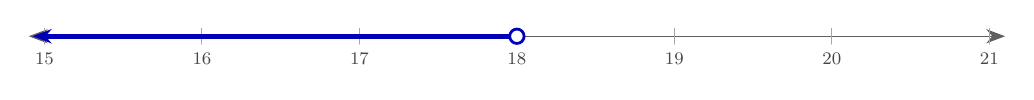
\begin{tikzpicture}[>={Stealth[length=2.4mm]},font=\footnotesize,line cap=round]
\draw[<->,gray!75!black] (-0.2,0) -- (12.2,0);
\draw[gray!70] (0,-0.1) -- (0,0.1);
\node[below,gray!55!black,scale=0.8] at (0,-0.12) {$15$};
\draw[gray!70] (2,-0.1) -- (2,0.1);
\node[below,gray!55!black,scale=0.8] at (2,-0.12) {$16$};
\draw[gray!70] (4,-0.1) -- (4,0.1);
\node[below,gray!55!black,scale=0.8] at (4,-0.12) {$17$};
\draw[gray!70] (6,-0.1) -- (6,0.1);
\node[below,gray!55!black,scale=0.8] at (6,-0.12) {$18$};
\draw[gray!70] (8,-0.1) -- (8,0.1);
\node[below,gray!55!black,scale=0.8] at (8,-0.12) {$19$};
\draw[gray!70] (10,-0.1) -- (10,0.1);
\node[below,gray!55!black,scale=0.8] at (10,-0.12) {$20$};
\draw[gray!70] (12,-0.1) -- (12,0.1);
\node[below,gray!55!black,scale=0.8] at (12,-0.12) {$21$};
\draw[blue!72!black,line width=1.8pt,->] (6,0) -- (-0.15,0);
\draw[blue!72!black,line width=1pt,fill=white] (6,0) circle (2.6pt);
\end{tikzpicture}
}
\end{center}
\medskip\hrule

\section*{Solving Linear Inequalities 29\quad\small\texttt{(ise1-029)}}
\addcontentsline{toc}{section}{Solving Linear Inequalities 29 (ise1-029)}
\textit{Difficulty: Foundation \quad\textbar\quad Marks: 3}

\question{Find the set of values of \( x \) which satisfy \( 2(5 - x) \geq 3(x - 1) \).}

\textbf{Worked solution.}

\textit{Step 1: Expand both brackets.}
\[\begin{gathered}
10 - 2x \geq 3x - 3
\end{gathered}\]
\( 2(5-x) = 10 - 2x \) and \( 3(x-1) = 3x - 3 \).

\textit{Step 2: Add \( 2x \) to both sides.}
\[\begin{gathered}
10 \geq 5x - 3
\end{gathered}\]
Collect \( x \) terms on the right.

\textit{Step 3: Add 3 to both sides.}
\[\begin{gathered}
13 \geq 5x
\end{gathered}\]
Isolate \( x \).

\textit{Step 4: Divide by 5.}
\[\begin{gathered}
\dfrac{13}{5} \geq x \quad \Rightarrow \quad x \leq \dfrac{13}{5}
\end{gathered}\]
Positive divisor --- direction unchanged.

\begin{answerbox}
\textbf{Final answer:}\quad \(\displaystyle  x \leq \dfrac{13}{5} \)
\end{answerbox}
\textbf{Solution on a number line.}

\begin{center}
\resizebox{\ifdim\width>\linewidth \linewidth\else \width\fi}{!}{%
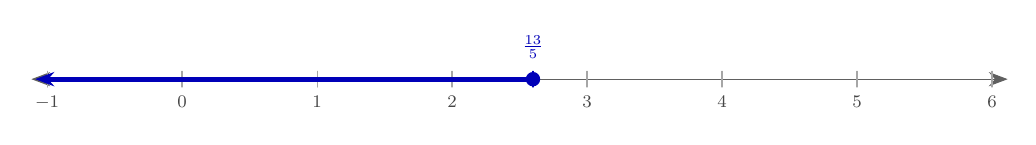
\begin{tikzpicture}[>={Stealth[length=2.4mm]},font=\footnotesize,line cap=round]
\draw[<->,gray!75!black] (-0.2,0) -- (12.2,0);
\draw[gray!70] (0,-0.1) -- (0,0.1);
\node[below,gray!55!black,scale=0.8] at (0,-0.12) {$-1$};
\draw[gray!70] (1.714,-0.1) -- (1.714,0.1);
\node[below,gray!55!black,scale=0.8] at (1.714,-0.12) {$0$};
\draw[gray!70] (3.429,-0.1) -- (3.429,0.1);
\node[below,gray!55!black,scale=0.8] at (3.429,-0.12) {$1$};
\draw[gray!70] (5.143,-0.1) -- (5.143,0.1);
\node[below,gray!55!black,scale=0.8] at (5.143,-0.12) {$2$};
\draw[gray!70] (6.857,-0.1) -- (6.857,0.1);
\node[below,gray!55!black,scale=0.8] at (6.857,-0.12) {$3$};
\draw[gray!70] (8.571,-0.1) -- (8.571,0.1);
\node[below,gray!55!black,scale=0.8] at (8.571,-0.12) {$4$};
\draw[gray!70] (10.286,-0.1) -- (10.286,0.1);
\node[below,gray!55!black,scale=0.8] at (10.286,-0.12) {$5$};
\draw[gray!70] (12,-0.1) -- (12,0.1);
\node[below,gray!55!black,scale=0.8] at (12,-0.12) {$6$};
\draw[blue!72!black,line width=1.8pt,->] (6.171,0) -- (-0.15,0);
\fill[blue!72!black] (6.171,0) circle (2.6pt);
\draw[blue!72!black] (6.171,-0.1) -- (6.171,0.1);
\node[above,blue!72!black,scale=0.82] at (6.171,0.16) {$\frac{13}{5}$};
\end{tikzpicture}
}
\end{center}
\medskip\hrule

\section*{Solving Linear Inequalities 30\quad\small\texttt{(ise1-030)}}
\addcontentsline{toc}{section}{Solving Linear Inequalities 30 (ise1-030)}
\textit{Difficulty: Foundation \quad\textbar\quad Marks: 3}

\question{Find the set of values of \( x \) which satisfy \( 6(x + 2) > 4(x + 5) \).}

\textbf{Worked solution.}

\textit{Step 1: Expand both brackets.}
\[\begin{gathered}
6x + 12 > 4x + 20
\end{gathered}\]
\( 6(x+2) = 6x+12 \) and \( 4(x+5) = 4x+20 \).

\textit{Step 2: Subtract \( 4x \) from both sides.}
\[\begin{gathered}
2x + 12 > 20
\end{gathered}\]
Collect \( x \) terms.

\textit{Step 3: Subtract 12 from both sides, then divide by 2.}
\[\begin{gathered}
2x > 8 \quad \Rightarrow \quad x > 4
\end{gathered}\]
Positive divisor --- direction unchanged.

\begin{answerbox}
\textbf{Final answer:}\quad \(\displaystyle  x > 4 \)
\end{answerbox}
\textbf{Solution on a number line.}

\begin{center}
\resizebox{\ifdim\width>\linewidth \linewidth\else \width\fi}{!}{%
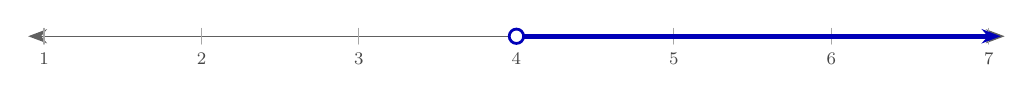
\begin{tikzpicture}[>={Stealth[length=2.4mm]},font=\footnotesize,line cap=round]
\draw[<->,gray!75!black] (-0.2,0) -- (12.2,0);
\draw[gray!70] (0,-0.1) -- (0,0.1);
\node[below,gray!55!black,scale=0.8] at (0,-0.12) {$1$};
\draw[gray!70] (2,-0.1) -- (2,0.1);
\node[below,gray!55!black,scale=0.8] at (2,-0.12) {$2$};
\draw[gray!70] (4,-0.1) -- (4,0.1);
\node[below,gray!55!black,scale=0.8] at (4,-0.12) {$3$};
\draw[gray!70] (6,-0.1) -- (6,0.1);
\node[below,gray!55!black,scale=0.8] at (6,-0.12) {$4$};
\draw[gray!70] (8,-0.1) -- (8,0.1);
\node[below,gray!55!black,scale=0.8] at (8,-0.12) {$5$};
\draw[gray!70] (10,-0.1) -- (10,0.1);
\node[below,gray!55!black,scale=0.8] at (10,-0.12) {$6$};
\draw[gray!70] (12,-0.1) -- (12,0.1);
\node[below,gray!55!black,scale=0.8] at (12,-0.12) {$7$};
\draw[blue!72!black,line width=1.8pt,->] (6,0) -- (12.15,0);
\draw[blue!72!black,line width=1pt,fill=white] (6,0) circle (2.6pt);
\end{tikzpicture}
}
\end{center}
\medskip\hrule

\section*{Solving Linear Inequalities 31\quad\small\texttt{(ise1-031)}}
\addcontentsline{toc}{section}{Solving Linear Inequalities 31 (ise1-031)}
\textit{Difficulty: Foundation \quad\textbar\quad Marks: 3}

\question{Find the set of values of \( x \) which satisfy \( 7(x - 3) \leq 5(x - 1) \). Give your answer in set notation.}

\textbf{Worked solution.}

\textit{Step 1: Expand both brackets.}
\[\begin{gathered}
7x - 21 \leq 5x - 5
\end{gathered}\]
\( 7(x-3) = 7x-21 \) and \( 5(x-1) = 5x-5 \).

\textit{Step 2: Subtract \( 5x \) from both sides.}
\[\begin{gathered}
2x - 21 \leq -5
\end{gathered}\]
Collect \( x \) terms.

\textit{Step 3: Add 21 to both sides.}
\[\begin{gathered}
2x \leq 16
\end{gathered}\]
Isolate \( x \).

\textit{Step 4: Divide by 2 and write in set notation.}
\[\begin{gathered}
x \leq 8 \quad \Rightarrow \quad \{x : x \leq 8\}
\end{gathered}\]
Solution expressed in set notation.

\begin{answerbox}
\textbf{Final answer:}\quad \(\displaystyle  \{x : x \leq 8\} \)
\end{answerbox}
\textbf{Solution on a number line.}

\begin{center}
\resizebox{\ifdim\width>\linewidth \linewidth\else \width\fi}{!}{%
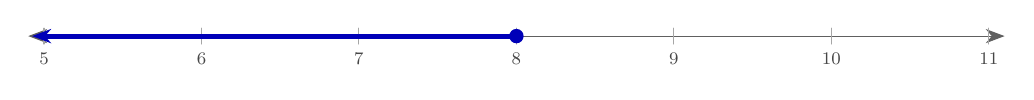
\begin{tikzpicture}[>={Stealth[length=2.4mm]},font=\footnotesize,line cap=round]
\draw[<->,gray!75!black] (-0.2,0) -- (12.2,0);
\draw[gray!70] (0,-0.1) -- (0,0.1);
\node[below,gray!55!black,scale=0.8] at (0,-0.12) {$5$};
\draw[gray!70] (2,-0.1) -- (2,0.1);
\node[below,gray!55!black,scale=0.8] at (2,-0.12) {$6$};
\draw[gray!70] (4,-0.1) -- (4,0.1);
\node[below,gray!55!black,scale=0.8] at (4,-0.12) {$7$};
\draw[gray!70] (6,-0.1) -- (6,0.1);
\node[below,gray!55!black,scale=0.8] at (6,-0.12) {$8$};
\draw[gray!70] (8,-0.1) -- (8,0.1);
\node[below,gray!55!black,scale=0.8] at (8,-0.12) {$9$};
\draw[gray!70] (10,-0.1) -- (10,0.1);
\node[below,gray!55!black,scale=0.8] at (10,-0.12) {$10$};
\draw[gray!70] (12,-0.1) -- (12,0.1);
\node[below,gray!55!black,scale=0.8] at (12,-0.12) {$11$};
\draw[blue!72!black,line width=1.8pt,->] (6,0) -- (-0.15,0);
\fill[blue!72!black] (6,0) circle (2.6pt);
\end{tikzpicture}
}
\end{center}
\medskip\hrule

\section*{Solving Linear Inequalities 32\quad\small\texttt{(ise1-032)}}
\addcontentsline{toc}{section}{Solving Linear Inequalities 32 (ise1-032)}
\textit{Difficulty: Foundation \quad\textbar\quad Marks: 3}

\question{Find the set of values of \( x \) which satisfy \( 3(4 - x) < 2(6 - x) \).}

\textbf{Worked solution.}

\textit{Step 1: Expand both brackets.}
\[\begin{gathered}
12 - 3x < 12 - 2x
\end{gathered}\]
\( 3(4-x) = 12-3x \) and \( 2(6-x) = 12-2x \).

\textit{Step 2: Add \( 3x \) to both sides.}
\[\begin{gathered}
12 < 12 + x
\end{gathered}\]
Collect \( x \) terms on the right.

\textit{Step 3: Subtract 12 from both sides.}
\[\begin{gathered}
0 < x \quad \Rightarrow \quad x > 0
\end{gathered}\]
Rewrite with \( x \) on the left.

\begin{answerbox}
\textbf{Final answer:}\quad \(\displaystyle  x > 0 \)
\end{answerbox}
\textbf{Solution on a number line.}

\begin{center}
\resizebox{\ifdim\width>\linewidth \linewidth\else \width\fi}{!}{%
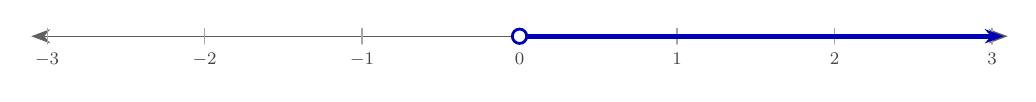
\begin{tikzpicture}[>={Stealth[length=2.4mm]},font=\footnotesize,line cap=round]
\draw[<->,gray!75!black] (-0.2,0) -- (12.2,0);
\draw[gray!70] (0,-0.1) -- (0,0.1);
\node[below,gray!55!black,scale=0.8] at (0,-0.12) {$-3$};
\draw[gray!70] (2,-0.1) -- (2,0.1);
\node[below,gray!55!black,scale=0.8] at (2,-0.12) {$-2$};
\draw[gray!70] (4,-0.1) -- (4,0.1);
\node[below,gray!55!black,scale=0.8] at (4,-0.12) {$-1$};
\draw[gray!70] (6,-0.1) -- (6,0.1);
\node[below,gray!55!black,scale=0.8] at (6,-0.12) {$0$};
\draw[gray!70] (8,-0.1) -- (8,0.1);
\node[below,gray!55!black,scale=0.8] at (8,-0.12) {$1$};
\draw[gray!70] (10,-0.1) -- (10,0.1);
\node[below,gray!55!black,scale=0.8] at (10,-0.12) {$2$};
\draw[gray!70] (12,-0.1) -- (12,0.1);
\node[below,gray!55!black,scale=0.8] at (12,-0.12) {$3$};
\draw[blue!72!black,line width=1.8pt,->] (6,0) -- (12.15,0);
\draw[blue!72!black,line width=1pt,fill=white] (6,0) circle (2.6pt);
\end{tikzpicture}
}
\end{center}
\medskip\hrule

\section*{Solving Linear Inequalities 33\quad\small\texttt{(ise1-033)}}
\addcontentsline{toc}{section}{Solving Linear Inequalities 33 (ise1-033)}
\textit{Difficulty: Foundation \quad\textbar\quad Marks: 3}

\question{Find the set of values of \( x \) which satisfy \( 4(3x - 2) \geq 2(5x + 1) \).}

\textbf{Worked solution.}

\textit{Step 1: Expand both brackets.}
\[\begin{gathered}
12x - 8 \geq 10x + 2
\end{gathered}\]
\( 4(3x-2) = 12x - 8 \) and \( 2(5x+1) = 10x + 2 \).

\textit{Step 2: Subtract \( 10x \) from both sides.}
\[\begin{gathered}
2x - 8 \geq 2
\end{gathered}\]
Collect \( x \) terms.

\textit{Step 3: Add 8 to both sides, then divide by 2.}
\[\begin{gathered}
2x \geq 10 \quad \Rightarrow \quad x \geq 5
\end{gathered}\]
Positive divisor --- direction unchanged.

\begin{answerbox}
\textbf{Final answer:}\quad \(\displaystyle  x \geq 5 \)
\end{answerbox}
\textbf{Solution on a number line.}

\begin{center}
\resizebox{\ifdim\width>\linewidth \linewidth\else \width\fi}{!}{%
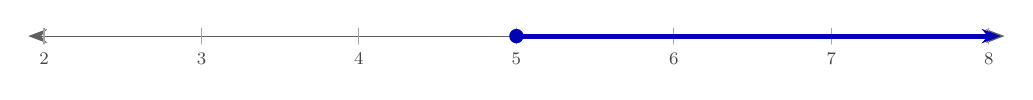
\begin{tikzpicture}[>={Stealth[length=2.4mm]},font=\footnotesize,line cap=round]
\draw[<->,gray!75!black] (-0.2,0) -- (12.2,0);
\draw[gray!70] (0,-0.1) -- (0,0.1);
\node[below,gray!55!black,scale=0.8] at (0,-0.12) {$2$};
\draw[gray!70] (2,-0.1) -- (2,0.1);
\node[below,gray!55!black,scale=0.8] at (2,-0.12) {$3$};
\draw[gray!70] (4,-0.1) -- (4,0.1);
\node[below,gray!55!black,scale=0.8] at (4,-0.12) {$4$};
\draw[gray!70] (6,-0.1) -- (6,0.1);
\node[below,gray!55!black,scale=0.8] at (6,-0.12) {$5$};
\draw[gray!70] (8,-0.1) -- (8,0.1);
\node[below,gray!55!black,scale=0.8] at (8,-0.12) {$6$};
\draw[gray!70] (10,-0.1) -- (10,0.1);
\node[below,gray!55!black,scale=0.8] at (10,-0.12) {$7$};
\draw[gray!70] (12,-0.1) -- (12,0.1);
\node[below,gray!55!black,scale=0.8] at (12,-0.12) {$8$};
\draw[blue!72!black,line width=1.8pt,->] (6,0) -- (12.15,0);
\fill[blue!72!black] (6,0) circle (2.6pt);
\end{tikzpicture}
}
\end{center}
\medskip\hrule

\section*{Solving Linear Inequalities 34\quad\small\texttt{(ise1-034)}}
\addcontentsline{toc}{section}{Solving Linear Inequalities 34 (ise1-034)}
\textit{Difficulty: Foundation \quad\textbar\quad Marks: 3}

\question{Find the set of values of \( x \) which satisfy \( 9(x - 2) > 5(x + 2) \). Give your answer in set notation.}

\textbf{Worked solution.}

\textit{Step 1: Expand both brackets.}
\[\begin{gathered}
9x - 18 > 5x + 10
\end{gathered}\]
\( 9(x-2) = 9x-18 \) and \( 5(x+2) = 5x+10 \).

\textit{Step 2: Subtract \( 5x \) from both sides.}
\[\begin{gathered}
4x - 18 > 10
\end{gathered}\]
Collect \( x \) terms.

\textit{Step 3: Add 18 to both sides, then divide by 4.}
\[\begin{gathered}
4x > 28 \quad \Rightarrow \quad x > 7
\end{gathered}\]
Positive divisor --- direction unchanged.

\textit{Step 4: Write in set notation.}
\[\begin{gathered}
\{x : x > 7\}
\end{gathered}\]
Solution in set notation.

\begin{answerbox}
\textbf{Final answer:}\quad \(\displaystyle  \{x : x > 7\} \)
\end{answerbox}
\textbf{Solution on a number line.}

\begin{center}
\resizebox{\ifdim\width>\linewidth \linewidth\else \width\fi}{!}{%
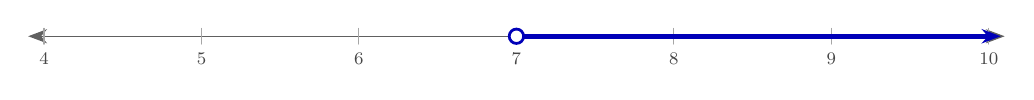
\begin{tikzpicture}[>={Stealth[length=2.4mm]},font=\footnotesize,line cap=round]
\draw[<->,gray!75!black] (-0.2,0) -- (12.2,0);
\draw[gray!70] (0,-0.1) -- (0,0.1);
\node[below,gray!55!black,scale=0.8] at (0,-0.12) {$4$};
\draw[gray!70] (2,-0.1) -- (2,0.1);
\node[below,gray!55!black,scale=0.8] at (2,-0.12) {$5$};
\draw[gray!70] (4,-0.1) -- (4,0.1);
\node[below,gray!55!black,scale=0.8] at (4,-0.12) {$6$};
\draw[gray!70] (6,-0.1) -- (6,0.1);
\node[below,gray!55!black,scale=0.8] at (6,-0.12) {$7$};
\draw[gray!70] (8,-0.1) -- (8,0.1);
\node[below,gray!55!black,scale=0.8] at (8,-0.12) {$8$};
\draw[gray!70] (10,-0.1) -- (10,0.1);
\node[below,gray!55!black,scale=0.8] at (10,-0.12) {$9$};
\draw[gray!70] (12,-0.1) -- (12,0.1);
\node[below,gray!55!black,scale=0.8] at (12,-0.12) {$10$};
\draw[blue!72!black,line width=1.8pt,->] (6,0) -- (12.15,0);
\draw[blue!72!black,line width=1pt,fill=white] (6,0) circle (2.6pt);
\end{tikzpicture}
}
\end{center}
\medskip\hrule

\section*{Solving Linear Inequalities 35\quad\small\texttt{(ise1-035)}}
\addcontentsline{toc}{section}{Solving Linear Inequalities 35 (ise1-035)}
\textit{Difficulty: Foundation \quad\textbar\quad Marks: 3}

\question{Find the set of values of \( x \) which satisfy \( 2(7 - 3x) < 4(2 - x) \). Give your answer in set notation.}

\textbf{Worked solution.}

\textit{Step 1: Expand both brackets.}
\[\begin{gathered}
14 - 6x < 8 - 4x
\end{gathered}\]
\( 2(7-3x) = 14-6x \) and \( 4(2-x) = 8-4x \).

\textit{Step 2: Add \( 6x \) to both sides.}
\[\begin{gathered}
14 < 8 + 2x
\end{gathered}\]
Eliminate \( x \) from the left.

\textit{Step 3: Subtract 8 from both sides.}
\[\begin{gathered}
6 < 2x
\end{gathered}\]
Isolate \( x \).

\textit{Step 4: Divide by 2 and write in set notation.}
\[\begin{gathered}
3 < x \quad \Rightarrow \quad \{x : x > 3\}
\end{gathered}\]
Rewrite with \( x \) on the left.

\begin{answerbox}
\textbf{Final answer:}\quad \(\displaystyle  \{x : x > 3\} \)
\end{answerbox}
\textbf{Solution on a number line.}

\begin{center}
\resizebox{\ifdim\width>\linewidth \linewidth\else \width\fi}{!}{%
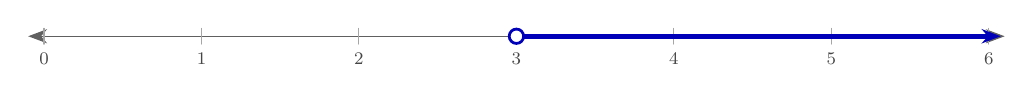
\begin{tikzpicture}[>={Stealth[length=2.4mm]},font=\footnotesize,line cap=round]
\draw[<->,gray!75!black] (-0.2,0) -- (12.2,0);
\draw[gray!70] (0,-0.1) -- (0,0.1);
\node[below,gray!55!black,scale=0.8] at (0,-0.12) {$0$};
\draw[gray!70] (2,-0.1) -- (2,0.1);
\node[below,gray!55!black,scale=0.8] at (2,-0.12) {$1$};
\draw[gray!70] (4,-0.1) -- (4,0.1);
\node[below,gray!55!black,scale=0.8] at (4,-0.12) {$2$};
\draw[gray!70] (6,-0.1) -- (6,0.1);
\node[below,gray!55!black,scale=0.8] at (6,-0.12) {$3$};
\draw[gray!70] (8,-0.1) -- (8,0.1);
\node[below,gray!55!black,scale=0.8] at (8,-0.12) {$4$};
\draw[gray!70] (10,-0.1) -- (10,0.1);
\node[below,gray!55!black,scale=0.8] at (10,-0.12) {$5$};
\draw[gray!70] (12,-0.1) -- (12,0.1);
\node[below,gray!55!black,scale=0.8] at (12,-0.12) {$6$};
\draw[blue!72!black,line width=1.8pt,->] (6,0) -- (12.15,0);
\draw[blue!72!black,line width=1pt,fill=white] (6,0) circle (2.6pt);
\end{tikzpicture}
}
\end{center}
\medskip\hrule

\section*{Solving Linear Inequalities 36\quad\small\texttt{(ise1-036)}}
\addcontentsline{toc}{section}{Solving Linear Inequalities 36 (ise1-036)}
\textit{Difficulty: Foundation \quad\textbar\quad Marks: 3}

\question{Find the set of values of \( x \) which satisfy \( \dfrac{x}{3} + 2 < 5 \).}

\textbf{Worked solution.}

\textit{Step 1: Subtract 2 from both sides.}
\[\begin{gathered}
\dfrac{x}{3} < 3
\end{gathered}\]
Isolate the fractional term.

\textit{Step 2: Multiply both sides by 3.}
\[\begin{gathered}
x < 9
\end{gathered}\]
Multiplying by a positive number keeps the direction.

\begin{answerbox}
\textbf{Final answer:}\quad \(\displaystyle  x < 9 \)
\end{answerbox}
\textbf{Solution on a number line.}

\begin{center}
\resizebox{\ifdim\width>\linewidth \linewidth\else \width\fi}{!}{%
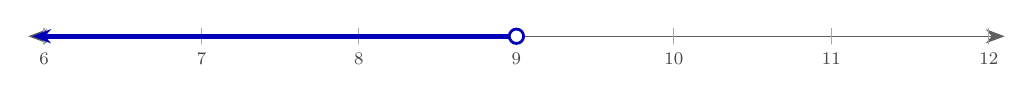
\begin{tikzpicture}[>={Stealth[length=2.4mm]},font=\footnotesize,line cap=round]
\draw[<->,gray!75!black] (-0.2,0) -- (12.2,0);
\draw[gray!70] (0,-0.1) -- (0,0.1);
\node[below,gray!55!black,scale=0.8] at (0,-0.12) {$6$};
\draw[gray!70] (2,-0.1) -- (2,0.1);
\node[below,gray!55!black,scale=0.8] at (2,-0.12) {$7$};
\draw[gray!70] (4,-0.1) -- (4,0.1);
\node[below,gray!55!black,scale=0.8] at (4,-0.12) {$8$};
\draw[gray!70] (6,-0.1) -- (6,0.1);
\node[below,gray!55!black,scale=0.8] at (6,-0.12) {$9$};
\draw[gray!70] (8,-0.1) -- (8,0.1);
\node[below,gray!55!black,scale=0.8] at (8,-0.12) {$10$};
\draw[gray!70] (10,-0.1) -- (10,0.1);
\node[below,gray!55!black,scale=0.8] at (10,-0.12) {$11$};
\draw[gray!70] (12,-0.1) -- (12,0.1);
\node[below,gray!55!black,scale=0.8] at (12,-0.12) {$12$};
\draw[blue!72!black,line width=1.8pt,->] (6,0) -- (-0.15,0);
\draw[blue!72!black,line width=1pt,fill=white] (6,0) circle (2.6pt);
\end{tikzpicture}
}
\end{center}
\medskip\hrule

\section*{Solving Linear Inequalities 37\quad\small\texttt{(ise1-037)}}
\addcontentsline{toc}{section}{Solving Linear Inequalities 37 (ise1-037)}
\textit{Difficulty: Foundation \quad\textbar\quad Marks: 3}

\question{Find the set of values of \( x \) which satisfy \( \dfrac{2x - 1}{4} \geq 3 \).}

\textbf{Worked solution.}

\textit{Step 1: Multiply both sides by 4.}
\[\begin{gathered}
2x - 1 \geq 12
\end{gathered}\]
Clear the denominator. Multiplying by a positive number keeps the direction.

\textit{Step 2: Add 1 to both sides.}
\[\begin{gathered}
2x \geq 13
\end{gathered}\]
Isolate \( x \).

\textit{Step 3: Divide by 2.}
\[\begin{gathered}
x \geq \dfrac{13}{2}
\end{gathered}\]
Solution found.

\begin{answerbox}
\textbf{Final answer:}\quad \(\displaystyle  x \geq \dfrac{13}{2} \)
\end{answerbox}
\textbf{Solution on a number line.}

\begin{center}
\resizebox{\ifdim\width>\linewidth \linewidth\else \width\fi}{!}{%
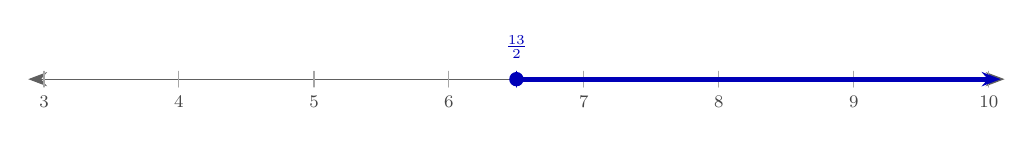
\begin{tikzpicture}[>={Stealth[length=2.4mm]},font=\footnotesize,line cap=round]
\draw[<->,gray!75!black] (-0.2,0) -- (12.2,0);
\draw[gray!70] (0,-0.1) -- (0,0.1);
\node[below,gray!55!black,scale=0.8] at (0,-0.12) {$3$};
\draw[gray!70] (1.714,-0.1) -- (1.714,0.1);
\node[below,gray!55!black,scale=0.8] at (1.714,-0.12) {$4$};
\draw[gray!70] (3.429,-0.1) -- (3.429,0.1);
\node[below,gray!55!black,scale=0.8] at (3.429,-0.12) {$5$};
\draw[gray!70] (5.143,-0.1) -- (5.143,0.1);
\node[below,gray!55!black,scale=0.8] at (5.143,-0.12) {$6$};
\draw[gray!70] (6.857,-0.1) -- (6.857,0.1);
\node[below,gray!55!black,scale=0.8] at (6.857,-0.12) {$7$};
\draw[gray!70] (8.571,-0.1) -- (8.571,0.1);
\node[below,gray!55!black,scale=0.8] at (8.571,-0.12) {$8$};
\draw[gray!70] (10.286,-0.1) -- (10.286,0.1);
\node[below,gray!55!black,scale=0.8] at (10.286,-0.12) {$9$};
\draw[gray!70] (12,-0.1) -- (12,0.1);
\node[below,gray!55!black,scale=0.8] at (12,-0.12) {$10$};
\draw[blue!72!black,line width=1.8pt,->] (6,0) -- (12.15,0);
\fill[blue!72!black] (6,0) circle (2.6pt);
\draw[blue!72!black] (6,-0.1) -- (6,0.1);
\node[above,blue!72!black,scale=0.82] at (6,0.16) {$\frac{13}{2}$};
\end{tikzpicture}
}
\end{center}
\medskip\hrule

\section*{Solving Linear Inequalities 38\quad\small\texttt{(ise1-038)}}
\addcontentsline{toc}{section}{Solving Linear Inequalities 38 (ise1-038)}
\textit{Difficulty: Foundation \quad\textbar\quad Marks: 3}

\question{Find the set of values of \( x \) which satisfy \( \dfrac{3x + 5}{2} < 7 \).}

\textbf{Worked solution.}

\textit{Step 1: Multiply both sides by 2.}
\[\begin{gathered}
3x + 5 < 14
\end{gathered}\]
Clear the denominator.

\textit{Step 2: Subtract 5 from both sides.}
\[\begin{gathered}
3x < 9
\end{gathered}\]
Isolate \( x \).

\textit{Step 3: Divide by 3.}
\[\begin{gathered}
x < 3
\end{gathered}\]
Solution found.

\begin{answerbox}
\textbf{Final answer:}\quad \(\displaystyle  x < 3 \)
\end{answerbox}
\textbf{Solution on a number line.}

\begin{center}
\resizebox{\ifdim\width>\linewidth \linewidth\else \width\fi}{!}{%
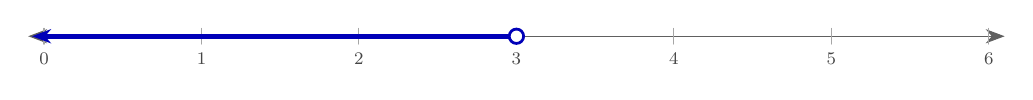
\begin{tikzpicture}[>={Stealth[length=2.4mm]},font=\footnotesize,line cap=round]
\draw[<->,gray!75!black] (-0.2,0) -- (12.2,0);
\draw[gray!70] (0,-0.1) -- (0,0.1);
\node[below,gray!55!black,scale=0.8] at (0,-0.12) {$0$};
\draw[gray!70] (2,-0.1) -- (2,0.1);
\node[below,gray!55!black,scale=0.8] at (2,-0.12) {$1$};
\draw[gray!70] (4,-0.1) -- (4,0.1);
\node[below,gray!55!black,scale=0.8] at (4,-0.12) {$2$};
\draw[gray!70] (6,-0.1) -- (6,0.1);
\node[below,gray!55!black,scale=0.8] at (6,-0.12) {$3$};
\draw[gray!70] (8,-0.1) -- (8,0.1);
\node[below,gray!55!black,scale=0.8] at (8,-0.12) {$4$};
\draw[gray!70] (10,-0.1) -- (10,0.1);
\node[below,gray!55!black,scale=0.8] at (10,-0.12) {$5$};
\draw[gray!70] (12,-0.1) -- (12,0.1);
\node[below,gray!55!black,scale=0.8] at (12,-0.12) {$6$};
\draw[blue!72!black,line width=1.8pt,->] (6,0) -- (-0.15,0);
\draw[blue!72!black,line width=1pt,fill=white] (6,0) circle (2.6pt);
\end{tikzpicture}
}
\end{center}
\medskip\hrule

\section*{Solving Linear Inequalities 39\quad\small\texttt{(ise1-039)}}
\addcontentsline{toc}{section}{Solving Linear Inequalities 39 (ise1-039)}
\textit{Difficulty: Foundation \quad\textbar\quad Marks: 3}

\question{Find the set of values of \( x \) which satisfy \( \dfrac{5 - x}{3} > 2 \).}

\textbf{Worked solution.}

\textit{Step 1: Multiply both sides by 3.}
\[\begin{gathered}
5 - x > 6
\end{gathered}\]
Clear the denominator.

\textit{Step 2: Subtract 5 from both sides.}
\[\begin{gathered}
-x > 1
\end{gathered}\]
Isolate \( x \).

\textit{Step 3: Multiply both sides by \( -1 \) and reverse the inequality.}
\[\begin{gathered}
x < -1
\end{gathered}\]
Multiplying by a negative reverses the inequality.

\begin{answerbox}
\textbf{Final answer:}\quad \(\displaystyle  x < -1 \)
\end{answerbox}
\textbf{Solution on a number line.}

\begin{center}
\resizebox{\ifdim\width>\linewidth \linewidth\else \width\fi}{!}{%
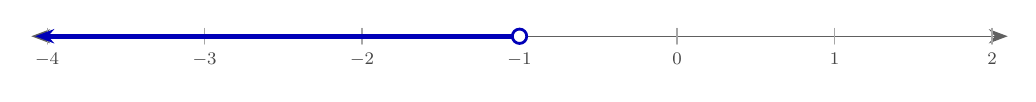
\begin{tikzpicture}[>={Stealth[length=2.4mm]},font=\footnotesize,line cap=round]
\draw[<->,gray!75!black] (-0.2,0) -- (12.2,0);
\draw[gray!70] (0,-0.1) -- (0,0.1);
\node[below,gray!55!black,scale=0.8] at (0,-0.12) {$-4$};
\draw[gray!70] (2,-0.1) -- (2,0.1);
\node[below,gray!55!black,scale=0.8] at (2,-0.12) {$-3$};
\draw[gray!70] (4,-0.1) -- (4,0.1);
\node[below,gray!55!black,scale=0.8] at (4,-0.12) {$-2$};
\draw[gray!70] (6,-0.1) -- (6,0.1);
\node[below,gray!55!black,scale=0.8] at (6,-0.12) {$-1$};
\draw[gray!70] (8,-0.1) -- (8,0.1);
\node[below,gray!55!black,scale=0.8] at (8,-0.12) {$0$};
\draw[gray!70] (10,-0.1) -- (10,0.1);
\node[below,gray!55!black,scale=0.8] at (10,-0.12) {$1$};
\draw[gray!70] (12,-0.1) -- (12,0.1);
\node[below,gray!55!black,scale=0.8] at (12,-0.12) {$2$};
\draw[blue!72!black,line width=1.8pt,->] (6,0) -- (-0.15,0);
\draw[blue!72!black,line width=1pt,fill=white] (6,0) circle (2.6pt);
\end{tikzpicture}
}
\end{center}
\medskip\hrule

\section*{Solving Linear Inequalities 40\quad\small\texttt{(ise1-040)}}
\addcontentsline{toc}{section}{Solving Linear Inequalities 40 (ise1-040)}
\textit{Difficulty: Foundation \quad\textbar\quad Marks: 4}

\question{Find the set of values of \( x \) which satisfy \( \dfrac{4x - 3}{5} \leq x - 1 \).}

\textbf{Worked solution.}

\textit{Step 1: Multiply both sides by 5.}
\[\begin{gathered}
4x - 3 \leq 5(x - 1)
\end{gathered}\]
Clear the denominator.

\textit{Step 2: Expand the right side.}
\[\begin{gathered}
4x - 3 \leq 5x - 5
\end{gathered}\]
\( 5(x-1) = 5x - 5 \).

\textit{Step 3: Subtract \( 4x \) from both sides.}
\[\begin{gathered}
-3 \leq x - 5
\end{gathered}\]
Collect \( x \) terms.

\textit{Step 4: Add 5 to both sides.}
\[\begin{gathered}
2 \leq x \quad \Rightarrow \quad x \geq 2
\end{gathered}\]
Rewrite with \( x \) on the left.

\begin{answerbox}
\textbf{Final answer:}\quad \(\displaystyle  x \geq 2 \)
\end{answerbox}
\textbf{Solution on a number line.}

\begin{center}
\resizebox{\ifdim\width>\linewidth \linewidth\else \width\fi}{!}{%
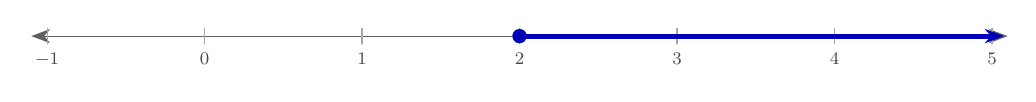
\begin{tikzpicture}[>={Stealth[length=2.4mm]},font=\footnotesize,line cap=round]
\draw[<->,gray!75!black] (-0.2,0) -- (12.2,0);
\draw[gray!70] (0,-0.1) -- (0,0.1);
\node[below,gray!55!black,scale=0.8] at (0,-0.12) {$-1$};
\draw[gray!70] (2,-0.1) -- (2,0.1);
\node[below,gray!55!black,scale=0.8] at (2,-0.12) {$0$};
\draw[gray!70] (4,-0.1) -- (4,0.1);
\node[below,gray!55!black,scale=0.8] at (4,-0.12) {$1$};
\draw[gray!70] (6,-0.1) -- (6,0.1);
\node[below,gray!55!black,scale=0.8] at (6,-0.12) {$2$};
\draw[gray!70] (8,-0.1) -- (8,0.1);
\node[below,gray!55!black,scale=0.8] at (8,-0.12) {$3$};
\draw[gray!70] (10,-0.1) -- (10,0.1);
\node[below,gray!55!black,scale=0.8] at (10,-0.12) {$4$};
\draw[gray!70] (12,-0.1) -- (12,0.1);
\node[below,gray!55!black,scale=0.8] at (12,-0.12) {$5$};
\draw[blue!72!black,line width=1.8pt,->] (6,0) -- (12.15,0);
\fill[blue!72!black] (6,0) circle (2.6pt);
\end{tikzpicture}
}
\end{center}
\medskip\hrule

\section*{Solving Linear Inequalities 41\quad\small\texttt{(ise1-041)}}
\addcontentsline{toc}{section}{Solving Linear Inequalities 41 (ise1-041)}
\textit{Difficulty: Foundation \quad\textbar\quad Marks: 4}

\question{Find the set of values of \( x \) which satisfy \( \dfrac{x + 3}{2} > \dfrac{x - 1}{3} \). Give your answer in set notation.}

\textbf{Worked solution.}

\textit{Step 1: Multiply both sides by 6 (LCM of 2 and 3) to clear both denominators.}
\[\begin{gathered}
3(x + 3) > 2(x - 1)
\end{gathered}\]
\( 6 \times \dfrac{x+3}{2} = 3(x+3) \) and \( 6 \times \dfrac{x-1}{3} = 2(x-1) \).

\textit{Step 2: Expand both brackets.}
\[\begin{gathered}
3x + 9 > 2x - 2
\end{gathered}\]
Remove brackets.

\textit{Step 3: Subtract \( 2x \) from both sides.}
\[\begin{gathered}
x + 9 > -2
\end{gathered}\]
Collect \( x \) terms.

\textit{Step 4: Subtract 9 from both sides and write in set notation.}
\[\begin{gathered}
x > -11 \quad \Rightarrow \quad \{x : x > -11\}
\end{gathered}\]
Solution expressed in set notation.

\begin{answerbox}
\textbf{Final answer:}\quad \(\displaystyle  \{x : x > -11\} \)
\end{answerbox}
\textbf{Solution on a number line.}

\begin{center}
\resizebox{\ifdim\width>\linewidth \linewidth\else \width\fi}{!}{%
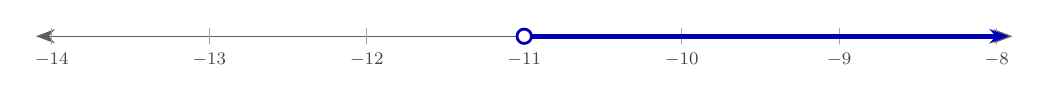
\begin{tikzpicture}[>={Stealth[length=2.4mm]},font=\footnotesize,line cap=round]
\draw[<->,gray!75!black] (-0.2,0) -- (12.2,0);
\draw[gray!70] (0,-0.1) -- (0,0.1);
\node[below,gray!55!black,scale=0.8] at (0,-0.12) {$-14$};
\draw[gray!70] (2,-0.1) -- (2,0.1);
\node[below,gray!55!black,scale=0.8] at (2,-0.12) {$-13$};
\draw[gray!70] (4,-0.1) -- (4,0.1);
\node[below,gray!55!black,scale=0.8] at (4,-0.12) {$-12$};
\draw[gray!70] (6,-0.1) -- (6,0.1);
\node[below,gray!55!black,scale=0.8] at (6,-0.12) {$-11$};
\draw[gray!70] (8,-0.1) -- (8,0.1);
\node[below,gray!55!black,scale=0.8] at (8,-0.12) {$-10$};
\draw[gray!70] (10,-0.1) -- (10,0.1);
\node[below,gray!55!black,scale=0.8] at (10,-0.12) {$-9$};
\draw[gray!70] (12,-0.1) -- (12,0.1);
\node[below,gray!55!black,scale=0.8] at (12,-0.12) {$-8$};
\draw[blue!72!black,line width=1.8pt,->] (6,0) -- (12.15,0);
\draw[blue!72!black,line width=1pt,fill=white] (6,0) circle (2.6pt);
\end{tikzpicture}
}
\end{center}
\medskip\hrule

\section*{Solving Linear Inequalities 42\quad\small\texttt{(ise1-042)}}
\addcontentsline{toc}{section}{Solving Linear Inequalities 42 (ise1-042)}
\textit{Difficulty: Foundation \quad\textbar\quad Marks: 4}

\question{Find the set of values of \( x \) which satisfy \( \dfrac{2x + 1}{3} \leq \dfrac{x + 4}{2} \).}

\textbf{Worked solution.}

\textit{Step 1: Multiply both sides by 6 (LCM of 2 and 3).}
\[\begin{gathered}
2(2x + 1) \leq 3(x + 4)
\end{gathered}\]
Clears both denominators simultaneously.

\textit{Step 2: Expand both brackets.}
\[\begin{gathered}
4x + 2 \leq 3x + 12
\end{gathered}\]
\( 2(2x+1) = 4x+2 \) and \( 3(x+4) = 3x+12 \).

\textit{Step 3: Subtract \( 3x \) from both sides.}
\[\begin{gathered}
x + 2 \leq 12
\end{gathered}\]
Collect \( x \) terms.

\textit{Step 4: Subtract 2 from both sides.}
\[\begin{gathered}
x \leq 10
\end{gathered}\]
Solution found.

\begin{answerbox}
\textbf{Final answer:}\quad \(\displaystyle  x \leq 10 \)
\end{answerbox}
\textbf{Solution on a number line.}

\begin{center}
\resizebox{\ifdim\width>\linewidth \linewidth\else \width\fi}{!}{%
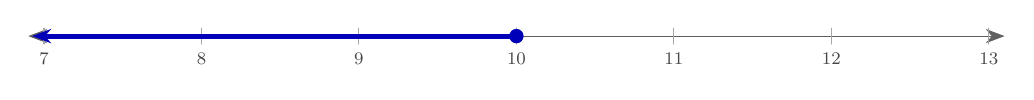
\begin{tikzpicture}[>={Stealth[length=2.4mm]},font=\footnotesize,line cap=round]
\draw[<->,gray!75!black] (-0.2,0) -- (12.2,0);
\draw[gray!70] (0,-0.1) -- (0,0.1);
\node[below,gray!55!black,scale=0.8] at (0,-0.12) {$7$};
\draw[gray!70] (2,-0.1) -- (2,0.1);
\node[below,gray!55!black,scale=0.8] at (2,-0.12) {$8$};
\draw[gray!70] (4,-0.1) -- (4,0.1);
\node[below,gray!55!black,scale=0.8] at (4,-0.12) {$9$};
\draw[gray!70] (6,-0.1) -- (6,0.1);
\node[below,gray!55!black,scale=0.8] at (6,-0.12) {$10$};
\draw[gray!70] (8,-0.1) -- (8,0.1);
\node[below,gray!55!black,scale=0.8] at (8,-0.12) {$11$};
\draw[gray!70] (10,-0.1) -- (10,0.1);
\node[below,gray!55!black,scale=0.8] at (10,-0.12) {$12$};
\draw[gray!70] (12,-0.1) -- (12,0.1);
\node[below,gray!55!black,scale=0.8] at (12,-0.12) {$13$};
\draw[blue!72!black,line width=1.8pt,->] (6,0) -- (-0.15,0);
\fill[blue!72!black] (6,0) circle (2.6pt);
\end{tikzpicture}
}
\end{center}
\medskip\hrule

\section*{Solving Linear Inequalities 43\quad\small\texttt{(ise1-043)}}
\addcontentsline{toc}{section}{Solving Linear Inequalities 43 (ise1-043)}
\textit{Difficulty: Foundation \quad\textbar\quad Marks: 4}

\question{Find the set of values of \( x \) which satisfy \( \dfrac{6 - 5x}{2} < \dfrac{4 - 8x}{3} \). Give your answer in set notation.}

\textbf{Worked solution.}

\textit{Step 1: Multiply both sides by 6 (LCM of 2 and 3).}
\[\begin{gathered}
3(6 - 5x) < 2(4 - 8x)
\end{gathered}\]
Clears both denominators.

\textit{Step 2: Expand both brackets.}
\[\begin{gathered}
18 - 15x < 8 - 16x
\end{gathered}\]
\( 3(6-5x) = 18-15x \) and \( 2(4-8x) = 8-16x \).

\textit{Step 3: Add \( 16x \) to both sides.}
\[\begin{gathered}
18 + x < 8
\end{gathered}\]
Collect \( x \) terms on the left.

\textit{Step 4: Subtract 18 from both sides and write in set notation.}
\[\begin{gathered}
x < -10 \quad \Rightarrow \quad \{x : x < -10\}
\end{gathered}\]
Solution in set notation.

\begin{answerbox}
\textbf{Final answer:}\quad \(\displaystyle  \{x : x < -10\} \)
\end{answerbox}
\textbf{Solution on a number line.}

\begin{center}
\resizebox{\ifdim\width>\linewidth \linewidth\else \width\fi}{!}{%
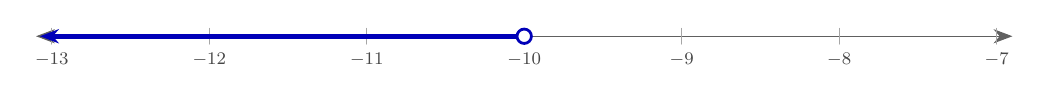
\begin{tikzpicture}[>={Stealth[length=2.4mm]},font=\footnotesize,line cap=round]
\draw[<->,gray!75!black] (-0.2,0) -- (12.2,0);
\draw[gray!70] (0,-0.1) -- (0,0.1);
\node[below,gray!55!black,scale=0.8] at (0,-0.12) {$-13$};
\draw[gray!70] (2,-0.1) -- (2,0.1);
\node[below,gray!55!black,scale=0.8] at (2,-0.12) {$-12$};
\draw[gray!70] (4,-0.1) -- (4,0.1);
\node[below,gray!55!black,scale=0.8] at (4,-0.12) {$-11$};
\draw[gray!70] (6,-0.1) -- (6,0.1);
\node[below,gray!55!black,scale=0.8] at (6,-0.12) {$-10$};
\draw[gray!70] (8,-0.1) -- (8,0.1);
\node[below,gray!55!black,scale=0.8] at (8,-0.12) {$-9$};
\draw[gray!70] (10,-0.1) -- (10,0.1);
\node[below,gray!55!black,scale=0.8] at (10,-0.12) {$-8$};
\draw[gray!70] (12,-0.1) -- (12,0.1);
\node[below,gray!55!black,scale=0.8] at (12,-0.12) {$-7$};
\draw[blue!72!black,line width=1.8pt,->] (6,0) -- (-0.15,0);
\draw[blue!72!black,line width=1pt,fill=white] (6,0) circle (2.6pt);
\end{tikzpicture}
}
\end{center}
\medskip\hrule

\section*{Solving Linear Inequalities 44\quad\small\texttt{(ise1-044)}}
\addcontentsline{toc}{section}{Solving Linear Inequalities 44 (ise1-044)}
\textit{Difficulty: Foundation \quad\textbar\quad Marks: 3}

\question{Find the set of values of \( x \) which satisfy \( \dfrac{3x - 1}{4} \geq 2x \).}

\textbf{Worked solution.}

\textit{Step 1: Multiply both sides by 4.}
\[\begin{gathered}
3x - 1 \geq 8x
\end{gathered}\]
Clear the denominator.

\textit{Step 2: Subtract \( 3x \) from both sides.}
\[\begin{gathered}
-1 \geq 5x
\end{gathered}\]
Collect \( x \) terms on the right.

\textit{Step 3: Divide by 5.}
\[\begin{gathered}
-\dfrac{1}{5} \geq x \quad \Rightarrow \quad x \leq -\dfrac{1}{5}
\end{gathered}\]
Positive divisor --- direction unchanged. Rewrite with \( x \) on the left.

\begin{answerbox}
\textbf{Final answer:}\quad \(\displaystyle  x \leq -\dfrac{1}{5} \)
\end{answerbox}
\textbf{Solution on a number line.}

\begin{center}
\resizebox{\ifdim\width>\linewidth \linewidth\else \width\fi}{!}{%
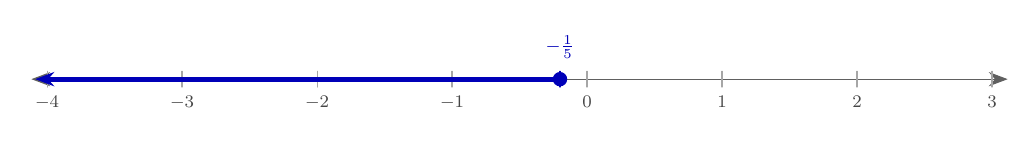
\begin{tikzpicture}[>={Stealth[length=2.4mm]},font=\footnotesize,line cap=round]
\draw[<->,gray!75!black] (-0.2,0) -- (12.2,0);
\draw[gray!70] (0,-0.1) -- (0,0.1);
\node[below,gray!55!black,scale=0.8] at (0,-0.12) {$-4$};
\draw[gray!70] (1.714,-0.1) -- (1.714,0.1);
\node[below,gray!55!black,scale=0.8] at (1.714,-0.12) {$-3$};
\draw[gray!70] (3.429,-0.1) -- (3.429,0.1);
\node[below,gray!55!black,scale=0.8] at (3.429,-0.12) {$-2$};
\draw[gray!70] (5.143,-0.1) -- (5.143,0.1);
\node[below,gray!55!black,scale=0.8] at (5.143,-0.12) {$-1$};
\draw[gray!70] (6.857,-0.1) -- (6.857,0.1);
\node[below,gray!55!black,scale=0.8] at (6.857,-0.12) {$0$};
\draw[gray!70] (8.571,-0.1) -- (8.571,0.1);
\node[below,gray!55!black,scale=0.8] at (8.571,-0.12) {$1$};
\draw[gray!70] (10.286,-0.1) -- (10.286,0.1);
\node[below,gray!55!black,scale=0.8] at (10.286,-0.12) {$2$};
\draw[gray!70] (12,-0.1) -- (12,0.1);
\node[below,gray!55!black,scale=0.8] at (12,-0.12) {$3$};
\draw[blue!72!black,line width=1.8pt,->] (6.514,0) -- (-0.15,0);
\fill[blue!72!black] (6.514,0) circle (2.6pt);
\draw[blue!72!black] (6.514,-0.1) -- (6.514,0.1);
\node[above,blue!72!black,scale=0.82] at (6.514,0.16) {$-\frac{1}{5}$};
\end{tikzpicture}
}
\end{center}
\medskip\hrule

\section*{Solving Linear Inequalities 45\quad\small\texttt{(ise1-045)}}
\addcontentsline{toc}{section}{Solving Linear Inequalities 45 (ise1-045)}
\textit{Difficulty: Foundation \quad\textbar\quad Marks: 4}

\question{Find the set of values of \( x \) which satisfy \( \dfrac{x - 2}{2} - \dfrac{2x + 3}{3} < 7 \). Give your answer in set notation.}

\textbf{Worked solution.}

\textit{Step 1: Multiply every term by 6 (LCM of 2 and 3).}
\[\begin{gathered}
3(x - 2) - 2(2x + 3) < 42
\end{gathered}\]
\( 6 \times \dfrac{x-2}{2} = 3(x-2) \) and \( 6 \times \dfrac{2x+3}{3} = 2(2x+3) \).

\textit{Step 2: Expand brackets.}
\[\begin{gathered}
3x - 6 - 4x - 6 < 42
\end{gathered}\]
\( 3(x-2) = 3x-6 \) and \( 2(2x+3) = 4x+6 \).

\textit{Step 3: Simplify the left side.}
\[\begin{gathered}
-x - 12 < 42
\end{gathered}\]
\( 3x - 4x = -x \) and \( -6 - 6 = -12 \).

\textit{Step 4: Add 12 to both sides, then divide by \(-1\) and reverse.}
\[\begin{gathered}
-x < 54 \quad \Rightarrow \quad x > -54
\end{gathered}\]
Dividing by \(-1\) reverses the inequality.

\textit{Step 5: Write in set notation.}
\[\begin{gathered}
\{x : x > -54\}
\end{gathered}\]
Solution in set notation.

\begin{answerbox}
\textbf{Final answer:}\quad \(\displaystyle  \{x : x > -54\} \)
\end{answerbox}
\textbf{Solution on a number line.}

\begin{center}
\resizebox{\ifdim\width>\linewidth \linewidth\else \width\fi}{!}{%
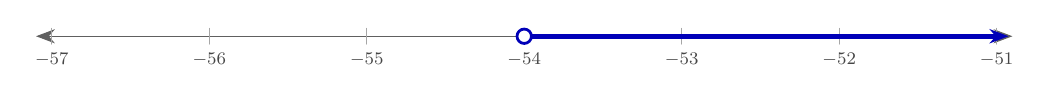
\begin{tikzpicture}[>={Stealth[length=2.4mm]},font=\footnotesize,line cap=round]
\draw[<->,gray!75!black] (-0.2,0) -- (12.2,0);
\draw[gray!70] (0,-0.1) -- (0,0.1);
\node[below,gray!55!black,scale=0.8] at (0,-0.12) {$-57$};
\draw[gray!70] (2,-0.1) -- (2,0.1);
\node[below,gray!55!black,scale=0.8] at (2,-0.12) {$-56$};
\draw[gray!70] (4,-0.1) -- (4,0.1);
\node[below,gray!55!black,scale=0.8] at (4,-0.12) {$-55$};
\draw[gray!70] (6,-0.1) -- (6,0.1);
\node[below,gray!55!black,scale=0.8] at (6,-0.12) {$-54$};
\draw[gray!70] (8,-0.1) -- (8,0.1);
\node[below,gray!55!black,scale=0.8] at (8,-0.12) {$-53$};
\draw[gray!70] (10,-0.1) -- (10,0.1);
\node[below,gray!55!black,scale=0.8] at (10,-0.12) {$-52$};
\draw[gray!70] (12,-0.1) -- (12,0.1);
\node[below,gray!55!black,scale=0.8] at (12,-0.12) {$-51$};
\draw[blue!72!black,line width=1.8pt,->] (6,0) -- (12.15,0);
\draw[blue!72!black,line width=1pt,fill=white] (6,0) circle (2.6pt);
\end{tikzpicture}
}
\end{center}
\medskip\hrule

\section*{Solving Linear Inequalities 46\quad\small\texttt{(ise1-046)}}
\addcontentsline{toc}{section}{Solving Linear Inequalities 46 (ise1-046)}
\textit{Difficulty: Foundation \quad\textbar\quad Marks: 3}

\question{Find the set of values of \( x \) which satisfy \( -3 < 2x + 1 \leq 9 \).}

\textbf{Worked solution.}

\textit{Step 1: Subtract 1 from all three parts.}
\[\begin{gathered}
-4 < 2x \leq 8
\end{gathered}\]
Treat all three parts simultaneously.

\textit{Step 2: Divide all three parts by 2.}
\[\begin{gathered}
-2 < x \leq 4
\end{gathered}\]
Positive divisor --- directions unchanged.

\begin{answerbox}
\textbf{Final answer:}\quad \(\displaystyle  -2 < x \leq 4 \)
\end{answerbox}
\textbf{Solution on a number line.}

\begin{center}
\resizebox{\ifdim\width>\linewidth \linewidth\else \width\fi}{!}{%
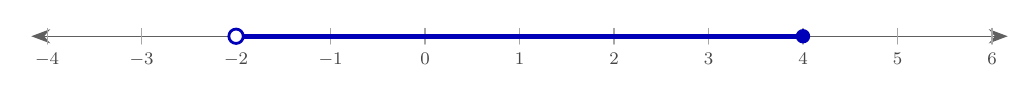
\begin{tikzpicture}[>={Stealth[length=2.4mm]},font=\footnotesize,line cap=round]
\draw[<->,gray!75!black] (-0.2,0) -- (12.2,0);
\draw[gray!70] (0,-0.1) -- (0,0.1);
\node[below,gray!55!black,scale=0.8] at (0,-0.12) {$-4$};
\draw[gray!70] (1.2,-0.1) -- (1.2,0.1);
\node[below,gray!55!black,scale=0.8] at (1.2,-0.12) {$-3$};
\draw[gray!70] (2.4,-0.1) -- (2.4,0.1);
\node[below,gray!55!black,scale=0.8] at (2.4,-0.12) {$-2$};
\draw[gray!70] (3.6,-0.1) -- (3.6,0.1);
\node[below,gray!55!black,scale=0.8] at (3.6,-0.12) {$-1$};
\draw[gray!70] (4.8,-0.1) -- (4.8,0.1);
\node[below,gray!55!black,scale=0.8] at (4.8,-0.12) {$0$};
\draw[gray!70] (6,-0.1) -- (6,0.1);
\node[below,gray!55!black,scale=0.8] at (6,-0.12) {$1$};
\draw[gray!70] (7.2,-0.1) -- (7.2,0.1);
\node[below,gray!55!black,scale=0.8] at (7.2,-0.12) {$2$};
\draw[gray!70] (8.4,-0.1) -- (8.4,0.1);
\node[below,gray!55!black,scale=0.8] at (8.4,-0.12) {$3$};
\draw[gray!70] (9.6,-0.1) -- (9.6,0.1);
\node[below,gray!55!black,scale=0.8] at (9.6,-0.12) {$4$};
\draw[gray!70] (10.8,-0.1) -- (10.8,0.1);
\node[below,gray!55!black,scale=0.8] at (10.8,-0.12) {$5$};
\draw[gray!70] (12,-0.1) -- (12,0.1);
\node[below,gray!55!black,scale=0.8] at (12,-0.12) {$6$};
\draw[blue!72!black,line width=1.8pt] (2.4,0) -- (9.6,0);
\draw[blue!72!black,line width=1pt,fill=white] (2.4,0) circle (2.6pt);
\fill[blue!72!black] (9.6,0) circle (2.6pt);
\end{tikzpicture}
}
\end{center}
\medskip\hrule

\section*{Solving Linear Inequalities 47\quad\small\texttt{(ise1-047)}}
\addcontentsline{toc}{section}{Solving Linear Inequalities 47 (ise1-047)}
\textit{Difficulty: Foundation \quad\textbar\quad Marks: 3}

\question{Find the set of values of \( x \) which satisfy \( 1 \leq 3x - 5 < 10 \).}

\textbf{Worked solution.}

\textit{Step 1: Add 5 to all three parts.}
\[\begin{gathered}
6 \leq 3x < 15
\end{gathered}\]
Apply the same operation throughout.

\textit{Step 2: Divide all three parts by 3.}
\[\begin{gathered}
2 \leq x < 5
\end{gathered}\]
Positive divisor --- directions unchanged.

\begin{answerbox}
\textbf{Final answer:}\quad \(\displaystyle  2 \leq x < 5 \)
\end{answerbox}
\textbf{Solution on a number line.}

\begin{center}
\resizebox{\ifdim\width>\linewidth \linewidth\else \width\fi}{!}{%
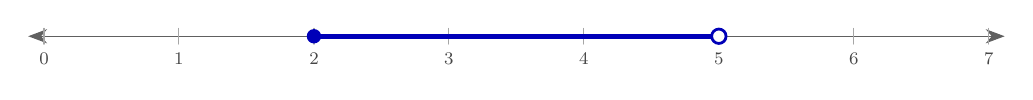
\begin{tikzpicture}[>={Stealth[length=2.4mm]},font=\footnotesize,line cap=round]
\draw[<->,gray!75!black] (-0.2,0) -- (12.2,0);
\draw[gray!70] (0,-0.1) -- (0,0.1);
\node[below,gray!55!black,scale=0.8] at (0,-0.12) {$0$};
\draw[gray!70] (1.714,-0.1) -- (1.714,0.1);
\node[below,gray!55!black,scale=0.8] at (1.714,-0.12) {$1$};
\draw[gray!70] (3.429,-0.1) -- (3.429,0.1);
\node[below,gray!55!black,scale=0.8] at (3.429,-0.12) {$2$};
\draw[gray!70] (5.143,-0.1) -- (5.143,0.1);
\node[below,gray!55!black,scale=0.8] at (5.143,-0.12) {$3$};
\draw[gray!70] (6.857,-0.1) -- (6.857,0.1);
\node[below,gray!55!black,scale=0.8] at (6.857,-0.12) {$4$};
\draw[gray!70] (8.571,-0.1) -- (8.571,0.1);
\node[below,gray!55!black,scale=0.8] at (8.571,-0.12) {$5$};
\draw[gray!70] (10.286,-0.1) -- (10.286,0.1);
\node[below,gray!55!black,scale=0.8] at (10.286,-0.12) {$6$};
\draw[gray!70] (12,-0.1) -- (12,0.1);
\node[below,gray!55!black,scale=0.8] at (12,-0.12) {$7$};
\draw[blue!72!black,line width=1.8pt] (3.429,0) -- (8.571,0);
\fill[blue!72!black] (3.429,0) circle (2.6pt);
\draw[blue!72!black,line width=1pt,fill=white] (8.571,0) circle (2.6pt);
\end{tikzpicture}
}
\end{center}
\medskip\hrule

\section*{Solving Linear Inequalities 48\quad\small\texttt{(ise1-048)}}
\addcontentsline{toc}{section}{Solving Linear Inequalities 48 (ise1-048)}
\textit{Difficulty: Foundation \quad\textbar\quad Marks: 3}

\question{Find the set of values of \( x \) which satisfy \( -5 \leq 4 - 3x < 10 \). Give your answer in set notation.}

\textbf{Worked solution.}

\textit{Step 1: Subtract 4 from all three parts.}
\[\begin{gathered}
-9 \leq -3x < 6
\end{gathered}\]
Apply the same operation throughout.

\textit{Step 2: Divide all three parts by \( -3 \) and reverse both inequality signs.}
\[\begin{gathered}
3 \geq x > -2
\end{gathered}\]
Dividing by a negative reverses all inequalities.

\textit{Step 3: Rewrite in conventional order and express in set notation.}
\[\begin{gathered}
-2 < x \leq 3 \quad \Rightarrow \quad \{x : -2 < x \leq 3\}
\end{gathered}\]
Write smaller value on the left.

\begin{answerbox}
\textbf{Final answer:}\quad \(\displaystyle  \{x : -2 < x \leq 3\} \)
\end{answerbox}
\textbf{Solution on a number line.}

\begin{center}
\resizebox{\ifdim\width>\linewidth \linewidth\else \width\fi}{!}{%
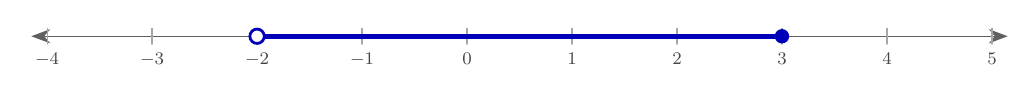
\begin{tikzpicture}[>={Stealth[length=2.4mm]},font=\footnotesize,line cap=round]
\draw[<->,gray!75!black] (-0.2,0) -- (12.2,0);
\draw[gray!70] (0,-0.1) -- (0,0.1);
\node[below,gray!55!black,scale=0.8] at (0,-0.12) {$-4$};
\draw[gray!70] (1.333,-0.1) -- (1.333,0.1);
\node[below,gray!55!black,scale=0.8] at (1.333,-0.12) {$-3$};
\draw[gray!70] (2.667,-0.1) -- (2.667,0.1);
\node[below,gray!55!black,scale=0.8] at (2.667,-0.12) {$-2$};
\draw[gray!70] (4,-0.1) -- (4,0.1);
\node[below,gray!55!black,scale=0.8] at (4,-0.12) {$-1$};
\draw[gray!70] (5.333,-0.1) -- (5.333,0.1);
\node[below,gray!55!black,scale=0.8] at (5.333,-0.12) {$0$};
\draw[gray!70] (6.667,-0.1) -- (6.667,0.1);
\node[below,gray!55!black,scale=0.8] at (6.667,-0.12) {$1$};
\draw[gray!70] (8,-0.1) -- (8,0.1);
\node[below,gray!55!black,scale=0.8] at (8,-0.12) {$2$};
\draw[gray!70] (9.333,-0.1) -- (9.333,0.1);
\node[below,gray!55!black,scale=0.8] at (9.333,-0.12) {$3$};
\draw[gray!70] (10.667,-0.1) -- (10.667,0.1);
\node[below,gray!55!black,scale=0.8] at (10.667,-0.12) {$4$};
\draw[gray!70] (12,-0.1) -- (12,0.1);
\node[below,gray!55!black,scale=0.8] at (12,-0.12) {$5$};
\draw[blue!72!black,line width=1.8pt] (2.667,0) -- (9.333,0);
\draw[blue!72!black,line width=1pt,fill=white] (2.667,0) circle (2.6pt);
\fill[blue!72!black] (9.333,0) circle (2.6pt);
\end{tikzpicture}
}
\end{center}
\medskip\hrule

\section*{Solving Linear Inequalities 49\quad\small\texttt{(ise1-049)}}
\addcontentsline{toc}{section}{Solving Linear Inequalities 49 (ise1-049)}
\textit{Difficulty: Foundation \quad\textbar\quad Marks: 3}

\question{Find the set of values of \( x \) which satisfy \( -1 < 5x + 4 < 19 \).}

\textbf{Worked solution.}

\textit{Step 1: Subtract 4 from all three parts.}
\[\begin{gathered}
-5 < 5x < 15
\end{gathered}\]
Apply to all parts.

\textit{Step 2: Divide all three parts by 5.}
\[\begin{gathered}
-1 < x < 3
\end{gathered}\]
Positive divisor --- directions unchanged.

\begin{answerbox}
\textbf{Final answer:}\quad \(\displaystyle  -1 < x < 3 \)
\end{answerbox}
\textbf{Solution on a number line.}

\begin{center}
\resizebox{\ifdim\width>\linewidth \linewidth\else \width\fi}{!}{%
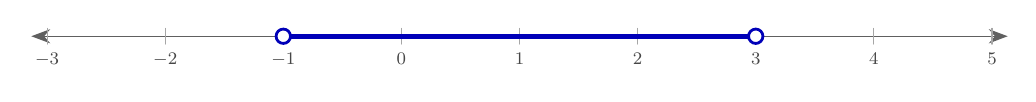
\begin{tikzpicture}[>={Stealth[length=2.4mm]},font=\footnotesize,line cap=round]
\draw[<->,gray!75!black] (-0.2,0) -- (12.2,0);
\draw[gray!70] (0,-0.1) -- (0,0.1);
\node[below,gray!55!black,scale=0.8] at (0,-0.12) {$-3$};
\draw[gray!70] (1.5,-0.1) -- (1.5,0.1);
\node[below,gray!55!black,scale=0.8] at (1.5,-0.12) {$-2$};
\draw[gray!70] (3,-0.1) -- (3,0.1);
\node[below,gray!55!black,scale=0.8] at (3,-0.12) {$-1$};
\draw[gray!70] (4.5,-0.1) -- (4.5,0.1);
\node[below,gray!55!black,scale=0.8] at (4.5,-0.12) {$0$};
\draw[gray!70] (6,-0.1) -- (6,0.1);
\node[below,gray!55!black,scale=0.8] at (6,-0.12) {$1$};
\draw[gray!70] (7.5,-0.1) -- (7.5,0.1);
\node[below,gray!55!black,scale=0.8] at (7.5,-0.12) {$2$};
\draw[gray!70] (9,-0.1) -- (9,0.1);
\node[below,gray!55!black,scale=0.8] at (9,-0.12) {$3$};
\draw[gray!70] (10.5,-0.1) -- (10.5,0.1);
\node[below,gray!55!black,scale=0.8] at (10.5,-0.12) {$4$};
\draw[gray!70] (12,-0.1) -- (12,0.1);
\node[below,gray!55!black,scale=0.8] at (12,-0.12) {$5$};
\draw[blue!72!black,line width=1.8pt] (3,0) -- (9,0);
\draw[blue!72!black,line width=1pt,fill=white] (3,0) circle (2.6pt);
\draw[blue!72!black,line width=1pt,fill=white] (9,0) circle (2.6pt);
\end{tikzpicture}
}
\end{center}
\medskip\hrule

\section*{Solving Linear Inequalities 50\quad\small\texttt{(ise1-050)}}
\addcontentsline{toc}{section}{Solving Linear Inequalities 50 (ise1-050)}
\textit{Difficulty: Foundation \quad\textbar\quad Marks: 3}

\question{Find the set of values of \( x \) which satisfy \( 7 \leq 3x - 2 < 16 \). Give your answer in set notation.}

\textbf{Worked solution.}

\textit{Step 1: Add 2 to all three parts.}
\[\begin{gathered}
9 \leq 3x < 18
\end{gathered}\]
Apply to all parts.

\textit{Step 2: Divide all three parts by 3 and write in set notation.}
\[\begin{gathered}
3 \leq x < 6 \quad \Rightarrow \quad \{x : 3 \leq x < 6\}
\end{gathered}\]
Positive divisor --- directions unchanged.

\begin{answerbox}
\textbf{Final answer:}\quad \(\displaystyle  \{x : 3 \leq x < 6\} \)
\end{answerbox}
\textbf{Solution on a number line.}

\begin{center}
\resizebox{\ifdim\width>\linewidth \linewidth\else \width\fi}{!}{%
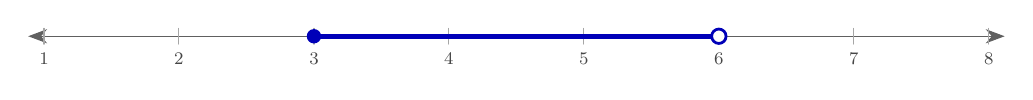
\begin{tikzpicture}[>={Stealth[length=2.4mm]},font=\footnotesize,line cap=round]
\draw[<->,gray!75!black] (-0.2,0) -- (12.2,0);
\draw[gray!70] (0,-0.1) -- (0,0.1);
\node[below,gray!55!black,scale=0.8] at (0,-0.12) {$1$};
\draw[gray!70] (1.714,-0.1) -- (1.714,0.1);
\node[below,gray!55!black,scale=0.8] at (1.714,-0.12) {$2$};
\draw[gray!70] (3.429,-0.1) -- (3.429,0.1);
\node[below,gray!55!black,scale=0.8] at (3.429,-0.12) {$3$};
\draw[gray!70] (5.143,-0.1) -- (5.143,0.1);
\node[below,gray!55!black,scale=0.8] at (5.143,-0.12) {$4$};
\draw[gray!70] (6.857,-0.1) -- (6.857,0.1);
\node[below,gray!55!black,scale=0.8] at (6.857,-0.12) {$5$};
\draw[gray!70] (8.571,-0.1) -- (8.571,0.1);
\node[below,gray!55!black,scale=0.8] at (8.571,-0.12) {$6$};
\draw[gray!70] (10.286,-0.1) -- (10.286,0.1);
\node[below,gray!55!black,scale=0.8] at (10.286,-0.12) {$7$};
\draw[gray!70] (12,-0.1) -- (12,0.1);
\node[below,gray!55!black,scale=0.8] at (12,-0.12) {$8$};
\draw[blue!72!black,line width=1.8pt] (3.429,0) -- (8.571,0);
\fill[blue!72!black] (3.429,0) circle (2.6pt);
\draw[blue!72!black,line width=1pt,fill=white] (8.571,0) circle (2.6pt);
\end{tikzpicture}
}
\end{center}
\medskip\hrule

\section*{Solving Linear Inequalities 51\quad\small\texttt{(ise1-051)}}
\addcontentsline{toc}{section}{Solving Linear Inequalities 51 (ise1-051)}
\textit{Difficulty: Foundation \quad\textbar\quad Marks: 3}

\question{Find the set of values of \( x \) which satisfy \( -7 < 2 - 3x \leq 14 \).}

\textbf{Worked solution.}

\textit{Step 1: Subtract 2 from all three parts.}
\[\begin{gathered}
-9 < -3x \leq 12
\end{gathered}\]
Apply the same operation.

\textit{Step 2: Divide by \( -3 \) and reverse both inequalities.}
\[\begin{gathered}
3 > x \geq -4
\end{gathered}\]
Dividing by a negative reverses all inequality signs.

\textit{Step 3: Rewrite in conventional order.}
\[\begin{gathered}
-4 \leq x < 3
\end{gathered}\]
Write smaller value on the left.

\begin{answerbox}
\textbf{Final answer:}\quad \(\displaystyle  -4 \leq x < 3 \)
\end{answerbox}
\textbf{Solution on a number line.}

\begin{center}
\resizebox{\ifdim\width>\linewidth \linewidth\else \width\fi}{!}{%
\begin{tikzpicture}[>={Stealth[length=2.4mm]},font=\footnotesize,line cap=round]
\draw[<->,gray!75!black] (-0.2,0) -- (12.2,0);
\draw[gray!70] (0,-0.1) -- (0,0.1);
\node[below,gray!55!black,scale=0.8] at (0,-0.12) {$-6$};
\draw[gray!70] (1.091,-0.1) -- (1.091,0.1);
\node[below,gray!55!black,scale=0.8] at (1.091,-0.12) {$-5$};
\draw[gray!70] (2.182,-0.1) -- (2.182,0.1);
\node[below,gray!55!black,scale=0.8] at (2.182,-0.12) {$-4$};
\draw[gray!70] (3.273,-0.1) -- (3.273,0.1);
\node[below,gray!55!black,scale=0.8] at (3.273,-0.12) {$-3$};
\draw[gray!70] (4.364,-0.1) -- (4.364,0.1);
\node[below,gray!55!black,scale=0.8] at (4.364,-0.12) {$-2$};
\draw[gray!70] (5.455,-0.1) -- (5.455,0.1);
\node[below,gray!55!black,scale=0.8] at (5.455,-0.12) {$-1$};
\draw[gray!70] (6.545,-0.1) -- (6.545,0.1);
\node[below,gray!55!black,scale=0.8] at (6.545,-0.12) {$0$};
\draw[gray!70] (7.636,-0.1) -- (7.636,0.1);
\node[below,gray!55!black,scale=0.8] at (7.636,-0.12) {$1$};
\draw[gray!70] (8.727,-0.1) -- (8.727,0.1);
\node[below,gray!55!black,scale=0.8] at (8.727,-0.12) {$2$};
\draw[gray!70] (9.818,-0.1) -- (9.818,0.1);
\node[below,gray!55!black,scale=0.8] at (9.818,-0.12) {$3$};
\draw[gray!70] (10.909,-0.1) -- (10.909,0.1);
\node[below,gray!55!black,scale=0.8] at (10.909,-0.12) {$4$};
\draw[gray!70] (12,-0.1) -- (12,0.1);
\node[below,gray!55!black,scale=0.8] at (12,-0.12) {$5$};
\draw[blue!72!black,line width=1.8pt] (2.182,0) -- (9.818,0);
\fill[blue!72!black] (2.182,0) circle (2.6pt);
\draw[blue!72!black,line width=1pt,fill=white] (9.818,0) circle (2.6pt);
\end{tikzpicture}
}
\end{center}
\medskip\hrule

\section*{Solving Linear Inequalities 52\quad\small\texttt{(ise1-052)}}
\addcontentsline{toc}{section}{Solving Linear Inequalities 52 (ise1-052)}
\textit{Difficulty: Foundation \quad\textbar\quad Marks: 3}

\question{Find the set of values of \( x \) which satisfy \( 5 \leq 7 + 6x \leq 11 \). Give your answer in set notation.}

\textbf{Worked solution.}

\textit{Step 1: Subtract 7 from all three parts.}
\[\begin{gathered}
-2 \leq 6x \leq 4
\end{gathered}\]
Apply the same operation.

\textit{Step 2: Divide all three parts by 6 and write in set notation.}
\[\begin{gathered}
-\dfrac{1}{3} \leq x \leq \dfrac{2}{3} \quad \Rightarrow \quad \{x : -\tfrac{1}{3} \leq x \leq \tfrac{2}{3}\}
\end{gathered}\]
Positive divisor --- directions unchanged.

\begin{answerbox}
\textbf{Final answer:}\quad \(\displaystyle  \{x : -\tfrac{1}{3} \leq x \leq \tfrac{2}{3}\} \)
\end{answerbox}
\textbf{Solution on a number line.}

\begin{center}
\resizebox{\ifdim\width>\linewidth \linewidth\else \width\fi}{!}{%
\begin{tikzpicture}[>={Stealth[length=2.4mm]},font=\footnotesize,line cap=round]
\draw[<->,gray!75!black] (-0.2,0) -- (12.2,0);
\draw[gray!70] (0,-0.1) -- (0,0.1);
\node[below,gray!55!black,scale=0.8] at (0,-0.12) {$-3$};
\draw[gray!70] (2,-0.1) -- (2,0.1);
\node[below,gray!55!black,scale=0.8] at (2,-0.12) {$-2$};
\draw[gray!70] (4,-0.1) -- (4,0.1);
\node[below,gray!55!black,scale=0.8] at (4,-0.12) {$-1$};
\draw[gray!70] (6,-0.1) -- (6,0.1);
\node[below,gray!55!black,scale=0.8] at (6,-0.12) {$0$};
\draw[gray!70] (8,-0.1) -- (8,0.1);
\node[below,gray!55!black,scale=0.8] at (8,-0.12) {$1$};
\draw[gray!70] (10,-0.1) -- (10,0.1);
\node[below,gray!55!black,scale=0.8] at (10,-0.12) {$2$};
\draw[gray!70] (12,-0.1) -- (12,0.1);
\node[below,gray!55!black,scale=0.8] at (12,-0.12) {$3$};
\draw[blue!72!black,line width=1.8pt] (5.333,0) -- (7.333,0);
\fill[blue!72!black] (5.333,0) circle (2.6pt);
\fill[blue!72!black] (7.333,0) circle (2.6pt);
\draw[blue!72!black] (5.333,-0.1) -- (5.333,0.1);
\node[above,blue!72!black,scale=0.82] at (5.333,0.16) {$-\frac{1}{3}$};
\draw[blue!72!black] (7.333,-0.1) -- (7.333,0.1);
\node[above,blue!72!black,scale=0.82] at (7.333,0.16) {$\frac{2}{3}$};
\end{tikzpicture}
}
\end{center}
\medskip\hrule

\section*{Solving Linear Inequalities 53\quad\small\texttt{(ise1-053)}}
\addcontentsline{toc}{section}{Solving Linear Inequalities 53 (ise1-053)}
\textit{Difficulty: Foundation \quad\textbar\quad Marks: 3}

\question{Find the set of values of \( x \) which satisfy \( -8 \leq 4 - 2x < 6 \).}

\textbf{Worked solution.}

\textit{Step 1: Subtract 4 from all three parts.}
\[\begin{gathered}
-12 \leq -2x < 2
\end{gathered}\]
Apply the same operation.

\textit{Step 2: Divide by \( -2 \) and reverse both inequality signs.}
\[\begin{gathered}
6 \geq x > -1
\end{gathered}\]
Dividing by a negative reverses all inequalities.

\textit{Step 3: Rewrite in conventional order.}
\[\begin{gathered}
-1 < x \leq 6
\end{gathered}\]
Write smaller value on the left.

\begin{answerbox}
\textbf{Final answer:}\quad \(\displaystyle  -1 < x \leq 6 \)
\end{answerbox}
\textbf{Solution on a number line.}

\begin{center}
\resizebox{\ifdim\width>\linewidth \linewidth\else \width\fi}{!}{%
\begin{tikzpicture}[>={Stealth[length=2.4mm]},font=\footnotesize,line cap=round]
\draw[<->,gray!75!black] (-0.2,0) -- (12.2,0);
\draw[gray!70] (0,-0.1) -- (0,0.1);
\node[below,gray!55!black,scale=0.8] at (0,-0.12) {$-3$};
\draw[gray!70] (1.091,-0.1) -- (1.091,0.1);
\node[below,gray!55!black,scale=0.8] at (1.091,-0.12) {$-2$};
\draw[gray!70] (2.182,-0.1) -- (2.182,0.1);
\node[below,gray!55!black,scale=0.8] at (2.182,-0.12) {$-1$};
\draw[gray!70] (3.273,-0.1) -- (3.273,0.1);
\node[below,gray!55!black,scale=0.8] at (3.273,-0.12) {$0$};
\draw[gray!70] (4.364,-0.1) -- (4.364,0.1);
\node[below,gray!55!black,scale=0.8] at (4.364,-0.12) {$1$};
\draw[gray!70] (5.455,-0.1) -- (5.455,0.1);
\node[below,gray!55!black,scale=0.8] at (5.455,-0.12) {$2$};
\draw[gray!70] (6.545,-0.1) -- (6.545,0.1);
\node[below,gray!55!black,scale=0.8] at (6.545,-0.12) {$3$};
\draw[gray!70] (7.636,-0.1) -- (7.636,0.1);
\node[below,gray!55!black,scale=0.8] at (7.636,-0.12) {$4$};
\draw[gray!70] (8.727,-0.1) -- (8.727,0.1);
\node[below,gray!55!black,scale=0.8] at (8.727,-0.12) {$5$};
\draw[gray!70] (9.818,-0.1) -- (9.818,0.1);
\node[below,gray!55!black,scale=0.8] at (9.818,-0.12) {$6$};
\draw[gray!70] (10.909,-0.1) -- (10.909,0.1);
\node[below,gray!55!black,scale=0.8] at (10.909,-0.12) {$7$};
\draw[gray!70] (12,-0.1) -- (12,0.1);
\node[below,gray!55!black,scale=0.8] at (12,-0.12) {$8$};
\draw[blue!72!black,line width=1.8pt] (2.182,0) -- (9.818,0);
\draw[blue!72!black,line width=1pt,fill=white] (2.182,0) circle (2.6pt);
\fill[blue!72!black] (9.818,0) circle (2.6pt);
\end{tikzpicture}
}
\end{center}
\medskip\hrule

\section*{Solving Linear Inequalities 54\quad\small\texttt{(ise1-054)}}
\addcontentsline{toc}{section}{Solving Linear Inequalities 54 (ise1-054)}
\textit{Difficulty: Foundation \quad\textbar\quad Marks: 3}

\question{Find the set of values of \( x \) which satisfy \( -5 < 2x - 3 < 15 \). Give your answer in set notation.}

\textbf{Worked solution.}

\textit{Step 1: Add 3 to all three parts.}
\[\begin{gathered}
-2 < 2x < 18
\end{gathered}\]
Apply the same operation.

\textit{Step 2: Divide all three parts by 2 and write in set notation.}
\[\begin{gathered}
-1 < x < 9 \quad \Rightarrow \quad \{x : -1 < x < 9\}
\end{gathered}\]
Positive divisor --- directions unchanged.

\begin{answerbox}
\textbf{Final answer:}\quad \(\displaystyle  \{x : -1 < x < 9\} \)
\end{answerbox}
\textbf{Solution on a number line.}

\begin{center}
\resizebox{\ifdim\width>\linewidth \linewidth\else \width\fi}{!}{%
\begin{tikzpicture}[>={Stealth[length=2.4mm]},font=\footnotesize,line cap=round]
\draw[<->,gray!75!black] (-0.2,0) -- (12.2,0);
\draw[gray!70] (0.857,-0.1) -- (0.857,0.1);
\node[below,gray!55!black,scale=0.8] at (0.857,-0.12) {$-2$};
\draw[gray!70] (2.571,-0.1) -- (2.571,0.1);
\node[below,gray!55!black,scale=0.8] at (2.571,-0.12) {$0$};
\draw[gray!70] (4.286,-0.1) -- (4.286,0.1);
\node[below,gray!55!black,scale=0.8] at (4.286,-0.12) {$2$};
\draw[gray!70] (6,-0.1) -- (6,0.1);
\node[below,gray!55!black,scale=0.8] at (6,-0.12) {$4$};
\draw[gray!70] (7.714,-0.1) -- (7.714,0.1);
\node[below,gray!55!black,scale=0.8] at (7.714,-0.12) {$6$};
\draw[gray!70] (9.429,-0.1) -- (9.429,0.1);
\node[below,gray!55!black,scale=0.8] at (9.429,-0.12) {$8$};
\draw[gray!70] (11.143,-0.1) -- (11.143,0.1);
\node[below,gray!55!black,scale=0.8] at (11.143,-0.12) {$10$};
\draw[blue!72!black,line width=1.8pt] (1.714,0) -- (10.286,0);
\draw[blue!72!black,line width=1pt,fill=white] (1.714,0) circle (2.6pt);
\draw[blue!72!black,line width=1pt,fill=white] (10.286,0) circle (2.6pt);
\end{tikzpicture}
}
\end{center}
\medskip\hrule

\section*{Solving Linear Inequalities 55\quad\small\texttt{(ise1-055)}}
\addcontentsline{toc}{section}{Solving Linear Inequalities 55 (ise1-055)}
\textit{Difficulty: Foundation \quad\textbar\quad Marks: 3}

\question{Find the set of values of \( x \) which satisfy \( -4 < \dfrac{x + 1}{2} \leq 3 \).}

\textbf{Worked solution.}

\textit{Step 1: Multiply all three parts by 2.}
\[\begin{gathered}
-8 < x + 1 \leq 6
\end{gathered}\]
Clear the denominator throughout.

\textit{Step 2: Subtract 1 from all three parts.}
\[\begin{gathered}
-9 < x \leq 5
\end{gathered}\]
Isolate \( x \).

\begin{answerbox}
\textbf{Final answer:}\quad \(\displaystyle  -9 < x \leq 5 \)
\end{answerbox}
\textbf{Solution on a number line.}

\begin{center}
\resizebox{\ifdim\width>\linewidth \linewidth\else \width\fi}{!}{%
\begin{tikzpicture}[>={Stealth[length=2.4mm]},font=\footnotesize,line cap=round]
\draw[<->,gray!75!black] (-0.2,0) -- (12.2,0);
\draw[gray!70] (0.667,-0.1) -- (0.667,0.1);
\node[below,gray!55!black,scale=0.8] at (0.667,-0.12) {$-10$};
\draw[gray!70] (2,-0.1) -- (2,0.1);
\node[below,gray!55!black,scale=0.8] at (2,-0.12) {$-8$};
\draw[gray!70] (3.333,-0.1) -- (3.333,0.1);
\node[below,gray!55!black,scale=0.8] at (3.333,-0.12) {$-6$};
\draw[gray!70] (4.667,-0.1) -- (4.667,0.1);
\node[below,gray!55!black,scale=0.8] at (4.667,-0.12) {$-4$};
\draw[gray!70] (6,-0.1) -- (6,0.1);
\node[below,gray!55!black,scale=0.8] at (6,-0.12) {$-2$};
\draw[gray!70] (7.333,-0.1) -- (7.333,0.1);
\node[below,gray!55!black,scale=0.8] at (7.333,-0.12) {$0$};
\draw[gray!70] (8.667,-0.1) -- (8.667,0.1);
\node[below,gray!55!black,scale=0.8] at (8.667,-0.12) {$2$};
\draw[gray!70] (10,-0.1) -- (10,0.1);
\node[below,gray!55!black,scale=0.8] at (10,-0.12) {$4$};
\draw[gray!70] (11.333,-0.1) -- (11.333,0.1);
\node[below,gray!55!black,scale=0.8] at (11.333,-0.12) {$6$};
\draw[blue!72!black,line width=1.8pt] (1.333,0) -- (10.667,0);
\draw[blue!72!black,line width=1pt,fill=white] (1.333,0) circle (2.6pt);
\fill[blue!72!black] (10.667,0) circle (2.6pt);
\end{tikzpicture}
}
\end{center}
\medskip\hrule

\section*{Solving Linear Inequalities 56\quad\small\texttt{(ise1-056)}}
\addcontentsline{toc}{section}{Solving Linear Inequalities 56 (ise1-056)}
\textit{Difficulty: Foundation \quad\textbar\quad Marks: 3}

\question{Find the set of values of \( x \) which satisfy \( 0 \leq \dfrac{3x - 6}{3} < 4 \). Give your answer in set notation.}

\textbf{Worked solution.}

\textit{Step 1: Multiply all three parts by 3.}
\[\begin{gathered}
0 \leq 3x - 6 < 12
\end{gathered}\]
Clear the denominator.

\textit{Step 2: Add 6 to all three parts.}
\[\begin{gathered}
6 \leq 3x < 18
\end{gathered}\]
Isolate the \( x \) term.

\textit{Step 3: Divide all three parts by 3 and write in set notation.}
\[\begin{gathered}
2 \leq x < 6 \quad \Rightarrow \quad \{x : 2 \leq x < 6\}
\end{gathered}\]
Positive divisor --- directions unchanged.

\begin{answerbox}
\textbf{Final answer:}\quad \(\displaystyle  \{x : 2 \leq x < 6\} \)
\end{answerbox}
\textbf{Solution on a number line.}

\begin{center}
\resizebox{\ifdim\width>\linewidth \linewidth\else \width\fi}{!}{%
\begin{tikzpicture}[>={Stealth[length=2.4mm]},font=\footnotesize,line cap=round]
\draw[<->,gray!75!black] (-0.2,0) -- (12.2,0);
\draw[gray!70] (0,-0.1) -- (0,0.1);
\node[below,gray!55!black,scale=0.8] at (0,-0.12) {$0$};
\draw[gray!70] (1.5,-0.1) -- (1.5,0.1);
\node[below,gray!55!black,scale=0.8] at (1.5,-0.12) {$1$};
\draw[gray!70] (3,-0.1) -- (3,0.1);
\node[below,gray!55!black,scale=0.8] at (3,-0.12) {$2$};
\draw[gray!70] (4.5,-0.1) -- (4.5,0.1);
\node[below,gray!55!black,scale=0.8] at (4.5,-0.12) {$3$};
\draw[gray!70] (6,-0.1) -- (6,0.1);
\node[below,gray!55!black,scale=0.8] at (6,-0.12) {$4$};
\draw[gray!70] (7.5,-0.1) -- (7.5,0.1);
\node[below,gray!55!black,scale=0.8] at (7.5,-0.12) {$5$};
\draw[gray!70] (9,-0.1) -- (9,0.1);
\node[below,gray!55!black,scale=0.8] at (9,-0.12) {$6$};
\draw[gray!70] (10.5,-0.1) -- (10.5,0.1);
\node[below,gray!55!black,scale=0.8] at (10.5,-0.12) {$7$};
\draw[gray!70] (12,-0.1) -- (12,0.1);
\node[below,gray!55!black,scale=0.8] at (12,-0.12) {$8$};
\draw[blue!72!black,line width=1.8pt] (3,0) -- (9,0);
\fill[blue!72!black] (3,0) circle (2.6pt);
\draw[blue!72!black,line width=1pt,fill=white] (9,0) circle (2.6pt);
\end{tikzpicture}
}
\end{center}
\medskip\hrule

\section*{Solving Linear Inequalities 57\quad\small\texttt{(ise1-057)}}
\addcontentsline{toc}{section}{Solving Linear Inequalities 57 (ise1-057)}
\textit{Difficulty: Foundation \quad\textbar\quad Marks: 3}

\question{Find the set of values of \( x \) which satisfy \( -2 \leq 5 - 4x < 13 \).}

\textbf{Worked solution.}

\textit{Step 1: Subtract 5 from all three parts.}
\[\begin{gathered}
-7 \leq -4x < 8
\end{gathered}\]
Apply the same operation.

\textit{Step 2: Divide by \( -4 \) and reverse both inequalities.}
\[\begin{gathered}
\dfrac{7}{4} \geq x > -2
\end{gathered}\]
Dividing by a negative reverses all inequality signs.

\textit{Step 3: Rewrite in conventional order.}
\[\begin{gathered}
-2 < x \leq \dfrac{7}{4}
\end{gathered}\]
Write smaller value on the left.

\begin{answerbox}
\textbf{Final answer:}\quad \(\displaystyle  -2 < x \leq \dfrac{7}{4} \)
\end{answerbox}
\textbf{Solution on a number line.}

\begin{center}
\resizebox{\ifdim\width>\linewidth \linewidth\else \width\fi}{!}{%
\begin{tikzpicture}[>={Stealth[length=2.4mm]},font=\footnotesize,line cap=round]
\draw[<->,gray!75!black] (-0.2,0) -- (12.2,0);
\draw[gray!70] (0,-0.1) -- (0,0.1);
\node[below,gray!55!black,scale=0.8] at (0,-0.12) {$-4$};
\draw[gray!70] (1.5,-0.1) -- (1.5,0.1);
\node[below,gray!55!black,scale=0.8] at (1.5,-0.12) {$-3$};
\draw[gray!70] (3,-0.1) -- (3,0.1);
\node[below,gray!55!black,scale=0.8] at (3,-0.12) {$-2$};
\draw[gray!70] (4.5,-0.1) -- (4.5,0.1);
\node[below,gray!55!black,scale=0.8] at (4.5,-0.12) {$-1$};
\draw[gray!70] (6,-0.1) -- (6,0.1);
\node[below,gray!55!black,scale=0.8] at (6,-0.12) {$0$};
\draw[gray!70] (7.5,-0.1) -- (7.5,0.1);
\node[below,gray!55!black,scale=0.8] at (7.5,-0.12) {$1$};
\draw[gray!70] (9,-0.1) -- (9,0.1);
\node[below,gray!55!black,scale=0.8] at (9,-0.12) {$2$};
\draw[gray!70] (10.5,-0.1) -- (10.5,0.1);
\node[below,gray!55!black,scale=0.8] at (10.5,-0.12) {$3$};
\draw[gray!70] (12,-0.1) -- (12,0.1);
\node[below,gray!55!black,scale=0.8] at (12,-0.12) {$4$};
\draw[blue!72!black,line width=1.8pt] (3,0) -- (8.625,0);
\draw[blue!72!black,line width=1pt,fill=white] (3,0) circle (2.6pt);
\fill[blue!72!black] (8.625,0) circle (2.6pt);
\draw[blue!72!black] (8.625,-0.1) -- (8.625,0.1);
\node[above,blue!72!black,scale=0.82] at (8.625,0.16) {$\frac{7}{4}$};
\end{tikzpicture}
}
\end{center}
\medskip\hrule

\section*{Solving Linear Inequalities 58\quad\small\texttt{(ise1-058)}}
\addcontentsline{toc}{section}{Solving Linear Inequalities 58 (ise1-058)}
\textit{Difficulty: Foundation \quad\textbar\quad Marks: 3}

\question{Find the set of values of \( x \) which satisfy \( -3 < 8 + 2x \leq 14 \). Give your answer in interval notation.}

\textbf{Worked solution.}

\textit{Step 1: Subtract 8 from all three parts.}
\[\begin{gathered}
-11 < 2x \leq 6
\end{gathered}\]
Apply the same operation.

\textit{Step 2: Divide all three parts by 2.}
\[\begin{gathered}
-\dfrac{11}{2} < x \leq 3
\end{gathered}\]
Positive divisor --- directions unchanged.

\textit{Step 3: Write in interval notation.}
\[\begin{gathered}
\left(-\dfrac{11}{2},\, 3\right]
\end{gathered}\]
Round bracket means \( -\tfrac{11}{2} \) is excluded; square bracket means 3 is included.

\begin{answerbox}
\textbf{Final answer:}\quad \(\displaystyle  \left(-\dfrac{11}{2},\, 3\right] \)
\end{answerbox}
\textbf{Solution on a number line.}

\begin{center}
\resizebox{\ifdim\width>\linewidth \linewidth\else \width\fi}{!}{%
\begin{tikzpicture}[>={Stealth[length=2.4mm]},font=\footnotesize,line cap=round]
\draw[<->,gray!75!black] (-0.2,0) -- (12.2,0);
\draw[gray!70] (0,-0.1) -- (0,0.1);
\node[below,gray!55!black,scale=0.8] at (0,-0.12) {$-8$};
\draw[gray!70] (0.923,-0.1) -- (0.923,0.1);
\node[below,gray!55!black,scale=0.8] at (0.923,-0.12) {$-7$};
\draw[gray!70] (1.846,-0.1) -- (1.846,0.1);
\node[below,gray!55!black,scale=0.8] at (1.846,-0.12) {$-6$};
\draw[gray!70] (2.769,-0.1) -- (2.769,0.1);
\node[below,gray!55!black,scale=0.8] at (2.769,-0.12) {$-5$};
\draw[gray!70] (3.692,-0.1) -- (3.692,0.1);
\node[below,gray!55!black,scale=0.8] at (3.692,-0.12) {$-4$};
\draw[gray!70] (4.615,-0.1) -- (4.615,0.1);
\node[below,gray!55!black,scale=0.8] at (4.615,-0.12) {$-3$};
\draw[gray!70] (5.538,-0.1) -- (5.538,0.1);
\node[below,gray!55!black,scale=0.8] at (5.538,-0.12) {$-2$};
\draw[gray!70] (6.462,-0.1) -- (6.462,0.1);
\node[below,gray!55!black,scale=0.8] at (6.462,-0.12) {$-1$};
\draw[gray!70] (7.385,-0.1) -- (7.385,0.1);
\node[below,gray!55!black,scale=0.8] at (7.385,-0.12) {$0$};
\draw[gray!70] (8.308,-0.1) -- (8.308,0.1);
\node[below,gray!55!black,scale=0.8] at (8.308,-0.12) {$1$};
\draw[gray!70] (9.231,-0.1) -- (9.231,0.1);
\node[below,gray!55!black,scale=0.8] at (9.231,-0.12) {$2$};
\draw[gray!70] (10.154,-0.1) -- (10.154,0.1);
\node[below,gray!55!black,scale=0.8] at (10.154,-0.12) {$3$};
\draw[gray!70] (11.077,-0.1) -- (11.077,0.1);
\node[below,gray!55!black,scale=0.8] at (11.077,-0.12) {$4$};
\draw[gray!70] (12,-0.1) -- (12,0.1);
\node[below,gray!55!black,scale=0.8] at (12,-0.12) {$5$};
\draw[blue!72!black,line width=1.8pt] (2.308,0) -- (10.154,0);
\draw[blue!72!black,line width=1pt,fill=white] (2.308,0) circle (2.6pt);
\fill[blue!72!black] (10.154,0) circle (2.6pt);
\draw[blue!72!black] (2.308,-0.1) -- (2.308,0.1);
\node[above,blue!72!black,scale=0.82] at (2.308,0.16) {$-\frac{11}{2}$};
\end{tikzpicture}
}
\end{center}
\medskip\hrule

\section*{Solving Linear Inequalities 59\quad\small\texttt{(ise1-059)}}
\addcontentsline{toc}{section}{Solving Linear Inequalities 59 (ise1-059)}
\textit{Difficulty: Foundation \quad\textbar\quad Marks: 3}

\question{Find the set of values of \( x \) which satisfy \( -10 \leq 3x + 2 \leq 17 \). Give your answer in interval notation.}

\textbf{Worked solution.}

\textit{Step 1: Subtract 2 from all three parts.}
\[\begin{gathered}
-12 \leq 3x \leq 15
\end{gathered}\]
Apply the same operation.

\textit{Step 2: Divide all three parts by 3.}
\[\begin{gathered}
-4 \leq x \leq 5
\end{gathered}\]
Positive divisor --- directions unchanged.

\textit{Step 3: Write in interval notation.}
\[\begin{gathered}
[-4,\, 5]
\end{gathered}\]
Square brackets on both sides since both endpoints are included.

\begin{answerbox}
\textbf{Final answer:}\quad \(\displaystyle  [-4,\, 5] \)
\end{answerbox}
\textbf{Solution on a number line.}

\begin{center}
\resizebox{\ifdim\width>\linewidth \linewidth\else \width\fi}{!}{%
\begin{tikzpicture}[>={Stealth[length=2.4mm]},font=\footnotesize,line cap=round]
\draw[<->,gray!75!black] (-0.2,0) -- (12.2,0);
\draw[gray!70] (0,-0.1) -- (0,0.1);
\node[below,gray!55!black,scale=0.8] at (0,-0.12) {$-6$};
\draw[gray!70] (0.923,-0.1) -- (0.923,0.1);
\node[below,gray!55!black,scale=0.8] at (0.923,-0.12) {$-5$};
\draw[gray!70] (1.846,-0.1) -- (1.846,0.1);
\node[below,gray!55!black,scale=0.8] at (1.846,-0.12) {$-4$};
\draw[gray!70] (2.769,-0.1) -- (2.769,0.1);
\node[below,gray!55!black,scale=0.8] at (2.769,-0.12) {$-3$};
\draw[gray!70] (3.692,-0.1) -- (3.692,0.1);
\node[below,gray!55!black,scale=0.8] at (3.692,-0.12) {$-2$};
\draw[gray!70] (4.615,-0.1) -- (4.615,0.1);
\node[below,gray!55!black,scale=0.8] at (4.615,-0.12) {$-1$};
\draw[gray!70] (5.538,-0.1) -- (5.538,0.1);
\node[below,gray!55!black,scale=0.8] at (5.538,-0.12) {$0$};
\draw[gray!70] (6.462,-0.1) -- (6.462,0.1);
\node[below,gray!55!black,scale=0.8] at (6.462,-0.12) {$1$};
\draw[gray!70] (7.385,-0.1) -- (7.385,0.1);
\node[below,gray!55!black,scale=0.8] at (7.385,-0.12) {$2$};
\draw[gray!70] (8.308,-0.1) -- (8.308,0.1);
\node[below,gray!55!black,scale=0.8] at (8.308,-0.12) {$3$};
\draw[gray!70] (9.231,-0.1) -- (9.231,0.1);
\node[below,gray!55!black,scale=0.8] at (9.231,-0.12) {$4$};
\draw[gray!70] (10.154,-0.1) -- (10.154,0.1);
\node[below,gray!55!black,scale=0.8] at (10.154,-0.12) {$5$};
\draw[gray!70] (11.077,-0.1) -- (11.077,0.1);
\node[below,gray!55!black,scale=0.8] at (11.077,-0.12) {$6$};
\draw[gray!70] (12,-0.1) -- (12,0.1);
\node[below,gray!55!black,scale=0.8] at (12,-0.12) {$7$};
\draw[blue!72!black,line width=1.8pt] (1.846,0) -- (10.154,0);
\fill[blue!72!black] (1.846,0) circle (2.6pt);
\fill[blue!72!black] (10.154,0) circle (2.6pt);
\end{tikzpicture}
}
\end{center}
\medskip\hrule

\section*{Solving Linear Inequalities 60\quad\small\texttt{(ise1-060)}}
\addcontentsline{toc}{section}{Solving Linear Inequalities 60 (ise1-060)}
\textit{Difficulty: Foundation \quad\textbar\quad Marks: 3}

\question{Find the set of values of \( x \) which satisfy \( -5 \leq 4 - 3x < 19 \). Give your answer in set notation.}

\textbf{Worked solution.}

\textit{Step 1: Subtract 4 from all three parts.}
\[\begin{gathered}
-9 \leq -3x < 15
\end{gathered}\]
Apply the same operation.

\textit{Step 2: Divide by \( -3 \) and reverse both inequality signs.}
\[\begin{gathered}
3 \geq x > -5
\end{gathered}\]
Dividing by a negative reverses all inequalities.

\textit{Step 3: Rewrite in conventional order and express in set notation.}
\[\begin{gathered}
-5 < x \leq 3 \quad \Rightarrow \quad \{x : -5 < x \leq 3\}
\end{gathered}\]
Write smaller value on the left.

\begin{answerbox}
\textbf{Final answer:}\quad \(\displaystyle  \{x : -5 < x \leq 3\} \)
\end{answerbox}
\textbf{Solution on a number line.}

\begin{center}
\resizebox{\ifdim\width>\linewidth \linewidth\else \width\fi}{!}{%
\begin{tikzpicture}[>={Stealth[length=2.4mm]},font=\footnotesize,line cap=round]
\draw[<->,gray!75!black] (-0.2,0) -- (12.2,0);
\draw[gray!70] (0,-0.1) -- (0,0.1);
\node[below,gray!55!black,scale=0.8] at (0,-0.12) {$-7$};
\draw[gray!70] (1,-0.1) -- (1,0.1);
\node[below,gray!55!black,scale=0.8] at (1,-0.12) {$-6$};
\draw[gray!70] (2,-0.1) -- (2,0.1);
\node[below,gray!55!black,scale=0.8] at (2,-0.12) {$-5$};
\draw[gray!70] (3,-0.1) -- (3,0.1);
\node[below,gray!55!black,scale=0.8] at (3,-0.12) {$-4$};
\draw[gray!70] (4,-0.1) -- (4,0.1);
\node[below,gray!55!black,scale=0.8] at (4,-0.12) {$-3$};
\draw[gray!70] (5,-0.1) -- (5,0.1);
\node[below,gray!55!black,scale=0.8] at (5,-0.12) {$-2$};
\draw[gray!70] (6,-0.1) -- (6,0.1);
\node[below,gray!55!black,scale=0.8] at (6,-0.12) {$-1$};
\draw[gray!70] (7,-0.1) -- (7,0.1);
\node[below,gray!55!black,scale=0.8] at (7,-0.12) {$0$};
\draw[gray!70] (8,-0.1) -- (8,0.1);
\node[below,gray!55!black,scale=0.8] at (8,-0.12) {$1$};
\draw[gray!70] (9,-0.1) -- (9,0.1);
\node[below,gray!55!black,scale=0.8] at (9,-0.12) {$2$};
\draw[gray!70] (10,-0.1) -- (10,0.1);
\node[below,gray!55!black,scale=0.8] at (10,-0.12) {$3$};
\draw[gray!70] (11,-0.1) -- (11,0.1);
\node[below,gray!55!black,scale=0.8] at (11,-0.12) {$4$};
\draw[gray!70] (12,-0.1) -- (12,0.1);
\node[below,gray!55!black,scale=0.8] at (12,-0.12) {$5$};
\draw[blue!72!black,line width=1.8pt] (2,0) -- (10,0);
\draw[blue!72!black,line width=1pt,fill=white] (2,0) circle (2.6pt);
\fill[blue!72!black] (10,0) circle (2.6pt);
\end{tikzpicture}
}
\end{center}
\medskip\hrule

\section*{Solving Linear Inequalities 61\quad\small\texttt{(ise1-061)}}
\addcontentsline{toc}{section}{Solving Linear Inequalities 61 (ise1-061)}
\textit{Difficulty: Foundation \quad\textbar\quad Marks: 4}

\question{Find the set of values of \( x \) which satisfy both \( 3x - 1 < x + 7 \) and \( 2x > x - 2 \). Give your answer in set notation.}

\textbf{Worked solution.}

\textit{Step 1: Solve the first inequality: \( 3x - 1 < x + 7 \).}
\[\begin{gathered}
2x < 8 \Rightarrow x < 4
\end{gathered}\]
Subtract \( x \), add 1, divide by 2.

\textit{Step 2: Solve the second inequality: \( 2x > x - 2 \).}
\[\begin{gathered}
x > -2
\end{gathered}\]
Subtract \( x \) from both sides.

\textit{Step 3: Combine: both conditions must hold simultaneously.}
\[\begin{gathered}
-2 < x < 4
\end{gathered}\]
The solution is the overlap of \( x > -2 \) and \( x < 4 \).

\textit{Step 4: Write in set notation.}
\[\begin{gathered}
\{x : -2 < x < 4\}
\end{gathered}\]
Both endpoints are strict (open) inequalities.

\begin{answerbox}
\textbf{Final answer:}\quad \(\displaystyle  \{x : -2 < x < 4\} \)
\end{answerbox}
\textbf{Solution on a number line.}

\begin{center}
\resizebox{\ifdim\width>\linewidth \linewidth\else \width\fi}{!}{%
\begin{tikzpicture}[>={Stealth[length=2.4mm]},font=\footnotesize,line cap=round]
\draw[<->,gray!75!black] (-0.2,0) -- (12.2,0);
\draw[gray!70] (0,-0.1) -- (0,0.1);
\node[below,gray!55!black,scale=0.8] at (0,-0.12) {$-4$};
\draw[gray!70] (1.2,-0.1) -- (1.2,0.1);
\node[below,gray!55!black,scale=0.8] at (1.2,-0.12) {$-3$};
\draw[gray!70] (2.4,-0.1) -- (2.4,0.1);
\node[below,gray!55!black,scale=0.8] at (2.4,-0.12) {$-2$};
\draw[gray!70] (3.6,-0.1) -- (3.6,0.1);
\node[below,gray!55!black,scale=0.8] at (3.6,-0.12) {$-1$};
\draw[gray!70] (4.8,-0.1) -- (4.8,0.1);
\node[below,gray!55!black,scale=0.8] at (4.8,-0.12) {$0$};
\draw[gray!70] (6,-0.1) -- (6,0.1);
\node[below,gray!55!black,scale=0.8] at (6,-0.12) {$1$};
\draw[gray!70] (7.2,-0.1) -- (7.2,0.1);
\node[below,gray!55!black,scale=0.8] at (7.2,-0.12) {$2$};
\draw[gray!70] (8.4,-0.1) -- (8.4,0.1);
\node[below,gray!55!black,scale=0.8] at (8.4,-0.12) {$3$};
\draw[gray!70] (9.6,-0.1) -- (9.6,0.1);
\node[below,gray!55!black,scale=0.8] at (9.6,-0.12) {$4$};
\draw[gray!70] (10.8,-0.1) -- (10.8,0.1);
\node[below,gray!55!black,scale=0.8] at (10.8,-0.12) {$5$};
\draw[gray!70] (12,-0.1) -- (12,0.1);
\node[below,gray!55!black,scale=0.8] at (12,-0.12) {$6$};
\draw[red!70!black,line width=1.1pt,->] (9.6,0.7) -- (-0.15,0.7);
\draw[red!70!black,line width=1pt,fill=white] (9.6,0.7) circle (2.6pt);
\node[right,red!70!black,scale=0.82] at (12.25,0.7) {$x<4$};
\draw[green!50!black,line width=1.1pt,->] (2.4,1.25) -- (12.15,1.25);
\draw[green!50!black,line width=1pt,fill=white] (2.4,1.25) circle (2.6pt);
\node[right,green!50!black,scale=0.82] at (12.25,1.25) {$x>-2$};
\draw[blue!72!black,line width=1.8pt] (2.4,0) -- (9.6,0);
\draw[blue!72!black,line width=1pt,fill=white] (2.4,0) circle (2.6pt);
\draw[blue!72!black,line width=1pt,fill=white] (9.6,0) circle (2.6pt);
\end{tikzpicture}
}
\end{center}
\medskip\hrule

\section*{Solving Linear Inequalities 62\quad\small\texttt{(ise1-062)}}
\addcontentsline{toc}{section}{Solving Linear Inequalities 62 (ise1-062)}
\textit{Difficulty: Foundation \quad\textbar\quad Marks: 4}

\question{Find the set of values of \( x \) which satisfy both \( 5x - 2 \leq 3x + 8 \) and \( 4x - 1 > x + 5 \). Give your answer in set notation.}

\textbf{Worked solution.}

\textit{Step 1: Solve \( 5x - 2 \leq 3x + 8 \).}
\[\begin{gathered}
2x \leq 10 \Rightarrow x \leq 5
\end{gathered}\]
Subtract \( 3x \), add 2, divide by 2.

\textit{Step 2: Solve \( 4x - 1 > x + 5 \).}
\[\begin{gathered}
3x > 6 \Rightarrow x > 2
\end{gathered}\]
Subtract \( x \), add 1, divide by 3.

\textit{Step 3: Combine both conditions.}
\[\begin{gathered}
2 < x \leq 5
\end{gathered}\]
Overlap of \( x > 2 \) and \( x \leq 5 \).

\textit{Step 4: Write in set notation.}
\[\begin{gathered}
\{x : 2 < x \leq 5\}
\end{gathered}\]
Open bracket at 2 (strict), closed at 5 (inclusive).

\begin{answerbox}
\textbf{Final answer:}\quad \(\displaystyle  \{x : 2 < x \leq 5\} \)
\end{answerbox}
\textbf{Solution on a number line.}

\begin{center}
\resizebox{\ifdim\width>\linewidth \linewidth\else \width\fi}{!}{%
\begin{tikzpicture}[>={Stealth[length=2.4mm]},font=\footnotesize,line cap=round]
\draw[<->,gray!75!black] (-0.2,0) -- (12.2,0);
\draw[gray!70] (0,-0.1) -- (0,0.1);
\node[below,gray!55!black,scale=0.8] at (0,-0.12) {$0$};
\draw[gray!70] (1.714,-0.1) -- (1.714,0.1);
\node[below,gray!55!black,scale=0.8] at (1.714,-0.12) {$1$};
\draw[gray!70] (3.429,-0.1) -- (3.429,0.1);
\node[below,gray!55!black,scale=0.8] at (3.429,-0.12) {$2$};
\draw[gray!70] (5.143,-0.1) -- (5.143,0.1);
\node[below,gray!55!black,scale=0.8] at (5.143,-0.12) {$3$};
\draw[gray!70] (6.857,-0.1) -- (6.857,0.1);
\node[below,gray!55!black,scale=0.8] at (6.857,-0.12) {$4$};
\draw[gray!70] (8.571,-0.1) -- (8.571,0.1);
\node[below,gray!55!black,scale=0.8] at (8.571,-0.12) {$5$};
\draw[gray!70] (10.286,-0.1) -- (10.286,0.1);
\node[below,gray!55!black,scale=0.8] at (10.286,-0.12) {$6$};
\draw[gray!70] (12,-0.1) -- (12,0.1);
\node[below,gray!55!black,scale=0.8] at (12,-0.12) {$7$};
\draw[red!70!black,line width=1.1pt,->] (8.571,0.7) -- (-0.15,0.7);
\fill[red!70!black] (8.571,0.7) circle (2.6pt);
\node[right,red!70!black,scale=0.82] at (12.25,0.7) {$x\le 5$};
\draw[green!50!black,line width=1.1pt,->] (3.429,1.25) -- (12.15,1.25);
\draw[green!50!black,line width=1pt,fill=white] (3.429,1.25) circle (2.6pt);
\node[right,green!50!black,scale=0.82] at (12.25,1.25) {$x>2$};
\draw[blue!72!black,line width=1.8pt] (3.429,0) -- (8.571,0);
\draw[blue!72!black,line width=1pt,fill=white] (3.429,0) circle (2.6pt);
\fill[blue!72!black] (8.571,0) circle (2.6pt);
\end{tikzpicture}
}
\end{center}
\medskip\hrule

\section*{Solving Linear Inequalities 63\quad\small\texttt{(ise1-063)}}
\addcontentsline{toc}{section}{Solving Linear Inequalities 63 (ise1-063)}
\textit{Difficulty: Foundation \quad\textbar\quad Marks: 4}

\question{Find the values of \( x \) which satisfy both \( 2x \geq 3x - 5 \) and \( 3x - 2 \geq x - 6 \). Give your answer in set notation.}

\textbf{Worked solution.}

\textit{Step 1: Solve \( 2x \geq 3x - 5 \).}
\[\begin{gathered}
5 \geq x \Rightarrow x \leq 5
\end{gathered}\]
Subtract \( 2x \) from both sides: \( 0 \geq x - 5 \Rightarrow 5 \geq x \).

\textit{Step 2: Solve \( 3x - 2 \geq x - 6 \).}
\[\begin{gathered}
2x \geq -4 \Rightarrow x \geq -2
\end{gathered}\]
Subtract \( x \), add 2, divide by 2.

\textit{Step 3: Combine both conditions.}
\[\begin{gathered}
-2 \leq x \leq 5
\end{gathered}\]
Overlap of \( x \geq -2 \) and \( x \leq 5 \).

\textit{Step 4: Write in set notation.}
\[\begin{gathered}
\{x : -2 \leq x \leq 5\}
\end{gathered}\]
Both endpoints are inclusive.

\begin{answerbox}
\textbf{Final answer:}\quad \(\displaystyle  \{x : -2 \leq x \leq 5\} \)
\end{answerbox}
\textbf{Solution on a number line.}

\begin{center}
\resizebox{\ifdim\width>\linewidth \linewidth\else \width\fi}{!}{%
\begin{tikzpicture}[>={Stealth[length=2.4mm]},font=\footnotesize,line cap=round]
\draw[<->,gray!75!black] (-0.2,0) -- (12.2,0);
\draw[gray!70] (0,-0.1) -- (0,0.1);
\node[below,gray!55!black,scale=0.8] at (0,-0.12) {$-4$};
\draw[gray!70] (1.091,-0.1) -- (1.091,0.1);
\node[below,gray!55!black,scale=0.8] at (1.091,-0.12) {$-3$};
\draw[gray!70] (2.182,-0.1) -- (2.182,0.1);
\node[below,gray!55!black,scale=0.8] at (2.182,-0.12) {$-2$};
\draw[gray!70] (3.273,-0.1) -- (3.273,0.1);
\node[below,gray!55!black,scale=0.8] at (3.273,-0.12) {$-1$};
\draw[gray!70] (4.364,-0.1) -- (4.364,0.1);
\node[below,gray!55!black,scale=0.8] at (4.364,-0.12) {$0$};
\draw[gray!70] (5.455,-0.1) -- (5.455,0.1);
\node[below,gray!55!black,scale=0.8] at (5.455,-0.12) {$1$};
\draw[gray!70] (6.545,-0.1) -- (6.545,0.1);
\node[below,gray!55!black,scale=0.8] at (6.545,-0.12) {$2$};
\draw[gray!70] (7.636,-0.1) -- (7.636,0.1);
\node[below,gray!55!black,scale=0.8] at (7.636,-0.12) {$3$};
\draw[gray!70] (8.727,-0.1) -- (8.727,0.1);
\node[below,gray!55!black,scale=0.8] at (8.727,-0.12) {$4$};
\draw[gray!70] (9.818,-0.1) -- (9.818,0.1);
\node[below,gray!55!black,scale=0.8] at (9.818,-0.12) {$5$};
\draw[gray!70] (10.909,-0.1) -- (10.909,0.1);
\node[below,gray!55!black,scale=0.8] at (10.909,-0.12) {$6$};
\draw[gray!70] (12,-0.1) -- (12,0.1);
\node[below,gray!55!black,scale=0.8] at (12,-0.12) {$7$};
\draw[red!70!black,line width=1.1pt,->] (9.818,0.7) -- (-0.15,0.7);
\fill[red!70!black] (9.818,0.7) circle (2.6pt);
\node[right,red!70!black,scale=0.82] at (12.25,0.7) {$x\le 5$};
\draw[green!50!black,line width=1.1pt,->] (2.182,1.25) -- (12.15,1.25);
\fill[green!50!black] (2.182,1.25) circle (2.6pt);
\node[right,green!50!black,scale=0.82] at (12.25,1.25) {$x\ge -2$};
\draw[blue!72!black,line width=1.8pt] (2.182,0) -- (9.818,0);
\fill[blue!72!black] (2.182,0) circle (2.6pt);
\fill[blue!72!black] (9.818,0) circle (2.6pt);
\end{tikzpicture}
}
\end{center}
\medskip\hrule

\section*{Solving Linear Inequalities 64\quad\small\texttt{(ise1-064)}}
\addcontentsline{toc}{section}{Solving Linear Inequalities 64 (ise1-064)}
\textit{Difficulty: Foundation \quad\textbar\quad Marks: 4}

\question{Find the values of \( x \) which satisfy both \( 4 - 2x < 10 \) and \( 3x - 1 < x + 7 \). Give your answer in set notation.}

\textbf{Worked solution.}

\textit{Step 1: Solve \( 4 - 2x < 10 \).}
\[\begin{gathered}
-2x < 6 \Rightarrow x > -3
\end{gathered}\]
Subtract 4, divide by \(-2\) and reverse.

\textit{Step 2: Solve \( 3x - 1 < x + 7 \).}
\[\begin{gathered}
2x < 8 \Rightarrow x < 4
\end{gathered}\]
Subtract \( x \), add 1, divide by 2.

\textit{Step 3: Combine both conditions and write in set notation.}
\[\begin{gathered}
-3 < x < 4 \quad \Rightarrow \quad \{x : -3 < x < 4\}
\end{gathered}\]
Both endpoints are strict (open).

\begin{answerbox}
\textbf{Final answer:}\quad \(\displaystyle  \{x : -3 < x < 4\} \)
\end{answerbox}
\textbf{Solution on a number line.}

\begin{center}
\resizebox{\ifdim\width>\linewidth \linewidth\else \width\fi}{!}{%
\begin{tikzpicture}[>={Stealth[length=2.4mm]},font=\footnotesize,line cap=round]
\draw[<->,gray!75!black] (-0.2,0) -- (12.2,0);
\draw[gray!70] (0,-0.1) -- (0,0.1);
\node[below,gray!55!black,scale=0.8] at (0,-0.12) {$-5$};
\draw[gray!70] (1.091,-0.1) -- (1.091,0.1);
\node[below,gray!55!black,scale=0.8] at (1.091,-0.12) {$-4$};
\draw[gray!70] (2.182,-0.1) -- (2.182,0.1);
\node[below,gray!55!black,scale=0.8] at (2.182,-0.12) {$-3$};
\draw[gray!70] (3.273,-0.1) -- (3.273,0.1);
\node[below,gray!55!black,scale=0.8] at (3.273,-0.12) {$-2$};
\draw[gray!70] (4.364,-0.1) -- (4.364,0.1);
\node[below,gray!55!black,scale=0.8] at (4.364,-0.12) {$-1$};
\draw[gray!70] (5.455,-0.1) -- (5.455,0.1);
\node[below,gray!55!black,scale=0.8] at (5.455,-0.12) {$0$};
\draw[gray!70] (6.545,-0.1) -- (6.545,0.1);
\node[below,gray!55!black,scale=0.8] at (6.545,-0.12) {$1$};
\draw[gray!70] (7.636,-0.1) -- (7.636,0.1);
\node[below,gray!55!black,scale=0.8] at (7.636,-0.12) {$2$};
\draw[gray!70] (8.727,-0.1) -- (8.727,0.1);
\node[below,gray!55!black,scale=0.8] at (8.727,-0.12) {$3$};
\draw[gray!70] (9.818,-0.1) -- (9.818,0.1);
\node[below,gray!55!black,scale=0.8] at (9.818,-0.12) {$4$};
\draw[gray!70] (10.909,-0.1) -- (10.909,0.1);
\node[below,gray!55!black,scale=0.8] at (10.909,-0.12) {$5$};
\draw[gray!70] (12,-0.1) -- (12,0.1);
\node[below,gray!55!black,scale=0.8] at (12,-0.12) {$6$};
\draw[red!70!black,line width=1.1pt,->] (2.182,0.7) -- (12.15,0.7);
\draw[red!70!black,line width=1pt,fill=white] (2.182,0.7) circle (2.6pt);
\node[right,red!70!black,scale=0.82] at (12.25,0.7) {$x>-3$};
\draw[green!50!black,line width=1.1pt,->] (9.818,1.25) -- (-0.15,1.25);
\draw[green!50!black,line width=1pt,fill=white] (9.818,1.25) circle (2.6pt);
\node[right,green!50!black,scale=0.82] at (12.25,1.25) {$x<4$};
\draw[blue!72!black,line width=1.8pt] (2.182,0) -- (9.818,0);
\draw[blue!72!black,line width=1pt,fill=white] (2.182,0) circle (2.6pt);
\draw[blue!72!black,line width=1pt,fill=white] (9.818,0) circle (2.6pt);
\end{tikzpicture}
}
\end{center}
\medskip\hrule

\section*{Solving Linear Inequalities 65\quad\small\texttt{(ise1-065)}}
\addcontentsline{toc}{section}{Solving Linear Inequalities 65 (ise1-065)}
\textit{Difficulty: Foundation \quad\textbar\quad Marks: 4}

\question{Find the values of \( x \) which satisfy both \( 5x + 1 \leq 11 \) and \( 2x - 3 < 5x - 6 \). Give your answer in set notation.}

\textbf{Worked solution.}

\textit{Step 1: Solve \( 5x + 1 \leq 11 \).}
\[\begin{gathered}
5x \leq 10 \Rightarrow x \leq 2
\end{gathered}\]
Subtract 1, divide by 5.

\textit{Step 2: Solve \( 2x - 3 < 5x - 6 \).}
\[\begin{gathered}
3 < 3x \Rightarrow x > 1
\end{gathered}\]
Subtract \( 2x \), add 6, divide by 3.

\textit{Step 3: Combine both conditions and write in set notation.}
\[\begin{gathered}
1 < x \leq 2 \quad \Rightarrow \quad \{x : 1 < x \leq 2\}
\end{gathered}\]
Overlap of \( x > 1 \) and \( x \leq 2 \).

\begin{answerbox}
\textbf{Final answer:}\quad \(\displaystyle  \{x : 1 < x \leq 2\} \)
\end{answerbox}
\textbf{Solution on a number line.}

\begin{center}
\resizebox{\ifdim\width>\linewidth \linewidth\else \width\fi}{!}{%
\begin{tikzpicture}[>={Stealth[length=2.4mm]},font=\footnotesize,line cap=round]
\draw[<->,gray!75!black] (-0.2,0) -- (12.2,0);
\draw[gray!70] (0,-0.1) -- (0,0.1);
\node[below,gray!55!black,scale=0.8] at (0,-0.12) {$-2$};
\draw[gray!70] (1.714,-0.1) -- (1.714,0.1);
\node[below,gray!55!black,scale=0.8] at (1.714,-0.12) {$-1$};
\draw[gray!70] (3.429,-0.1) -- (3.429,0.1);
\node[below,gray!55!black,scale=0.8] at (3.429,-0.12) {$0$};
\draw[gray!70] (5.143,-0.1) -- (5.143,0.1);
\node[below,gray!55!black,scale=0.8] at (5.143,-0.12) {$1$};
\draw[gray!70] (6.857,-0.1) -- (6.857,0.1);
\node[below,gray!55!black,scale=0.8] at (6.857,-0.12) {$2$};
\draw[gray!70] (8.571,-0.1) -- (8.571,0.1);
\node[below,gray!55!black,scale=0.8] at (8.571,-0.12) {$3$};
\draw[gray!70] (10.286,-0.1) -- (10.286,0.1);
\node[below,gray!55!black,scale=0.8] at (10.286,-0.12) {$4$};
\draw[gray!70] (12,-0.1) -- (12,0.1);
\node[below,gray!55!black,scale=0.8] at (12,-0.12) {$5$};
\draw[red!70!black,line width=1.1pt,->] (6.857,0.7) -- (-0.15,0.7);
\fill[red!70!black] (6.857,0.7) circle (2.6pt);
\node[right,red!70!black,scale=0.82] at (12.25,0.7) {$x\le 2$};
\draw[green!50!black,line width=1.1pt,->] (5.143,1.25) -- (12.15,1.25);
\draw[green!50!black,line width=1pt,fill=white] (5.143,1.25) circle (2.6pt);
\node[right,green!50!black,scale=0.82] at (12.25,1.25) {$x>1$};
\draw[blue!72!black,line width=1.8pt] (5.143,0) -- (6.857,0);
\draw[blue!72!black,line width=1pt,fill=white] (5.143,0) circle (2.6pt);
\fill[blue!72!black] (6.857,0) circle (2.6pt);
\end{tikzpicture}
}
\end{center}
\medskip\hrule

\section*{Solving Linear Inequalities 66\quad\small\texttt{(ise1-066)}}
\addcontentsline{toc}{section}{Solving Linear Inequalities 66 (ise1-066)}
\textit{Difficulty: Foundation \quad\textbar\quad Marks: 4}

\question{Find the values of \( x \) which satisfy both \( 2x - 1 \leq 3x - 5 \) and \( 5x - 6 > x + 22 \). Give your answer in set notation.}

\textbf{Worked solution.}

\textit{Step 1: Solve \( 2x - 1 \leq 3x - 5 \).}
\[\begin{gathered}
4 \leq x \Rightarrow x \geq 4
\end{gathered}\]
Subtract \( 2x \), add 5: \( 4 \leq x \).

\textit{Step 2: Solve \( 5x - 6 > x + 22 \).}
\[\begin{gathered}
4x > 28 \Rightarrow x > 7
\end{gathered}\]
Subtract \( x \), add 6, divide by 4.

\textit{Step 3: Combine both conditions.}
\[\begin{gathered}
x > 7
\end{gathered}\]
Since \( x > 7 \) is more restrictive than \( x \geq 4 \), the overlap is \( x > 7 \).

\textit{Step 4: Write in set notation.}
\[\begin{gathered}
\{x : x > 7\}
\end{gathered}\]
Only the stricter condition applies.

\begin{answerbox}
\textbf{Final answer:}\quad \(\displaystyle  \{x : x > 7\} \)
\end{answerbox}
\textbf{Solution on a number line.}

\begin{center}
\resizebox{\ifdim\width>\linewidth \linewidth\else \width\fi}{!}{%
\begin{tikzpicture}[>={Stealth[length=2.4mm]},font=\footnotesize,line cap=round]
\draw[<->,gray!75!black] (-0.2,0) -- (12.2,0);
\draw[gray!70] (0,-0.1) -- (0,0.1);
\node[below,gray!55!black,scale=0.8] at (0,-0.12) {$2$};
\draw[gray!70] (1.714,-0.1) -- (1.714,0.1);
\node[below,gray!55!black,scale=0.8] at (1.714,-0.12) {$3$};
\draw[gray!70] (3.429,-0.1) -- (3.429,0.1);
\node[below,gray!55!black,scale=0.8] at (3.429,-0.12) {$4$};
\draw[gray!70] (5.143,-0.1) -- (5.143,0.1);
\node[below,gray!55!black,scale=0.8] at (5.143,-0.12) {$5$};
\draw[gray!70] (6.857,-0.1) -- (6.857,0.1);
\node[below,gray!55!black,scale=0.8] at (6.857,-0.12) {$6$};
\draw[gray!70] (8.571,-0.1) -- (8.571,0.1);
\node[below,gray!55!black,scale=0.8] at (8.571,-0.12) {$7$};
\draw[gray!70] (10.286,-0.1) -- (10.286,0.1);
\node[below,gray!55!black,scale=0.8] at (10.286,-0.12) {$8$};
\draw[gray!70] (12,-0.1) -- (12,0.1);
\node[below,gray!55!black,scale=0.8] at (12,-0.12) {$9$};
\draw[red!70!black,line width=1.1pt,->] (3.429,0.7) -- (12.15,0.7);
\fill[red!70!black] (3.429,0.7) circle (2.6pt);
\node[right,red!70!black,scale=0.82] at (12.25,0.7) {$x\ge 4$};
\draw[green!50!black,line width=1.1pt,->] (8.571,1.25) -- (12.15,1.25);
\draw[green!50!black,line width=1pt,fill=white] (8.571,1.25) circle (2.6pt);
\node[right,green!50!black,scale=0.82] at (12.25,1.25) {$x>7$};
\draw[blue!72!black,line width=1.8pt,->] (8.571,0) -- (12.15,0);
\draw[blue!72!black,line width=1pt,fill=white] (8.571,0) circle (2.6pt);
\end{tikzpicture}
}
\end{center}
\medskip\hrule

\section*{Solving Linear Inequalities 67\quad\small\texttt{(ise1-067)}}
\addcontentsline{toc}{section}{Solving Linear Inequalities 67 (ise1-067)}
\textit{Difficulty: Foundation \quad\textbar\quad Marks: 4}

\question{Find the values of \( x \) which satisfy both \( 3x + 5 < x + 1 \) and \( 6x - 1 \geq 3x + 5 \). Give your answer in set notation.}

\textbf{Worked solution.}

\textit{Step 1: Solve \( 3x + 5 < x + 1 \).}
\[\begin{gathered}
2x < -4 \Rightarrow x < -2
\end{gathered}\]
Subtract \( x \) and 5, divide by 2.

\textit{Step 2: Solve \( 6x - 1 \geq 3x + 5 \).}
\[\begin{gathered}
3x \geq 6 \Rightarrow x \geq 2
\end{gathered}\]
Subtract \( 3x \), add 1, divide by 3.

\textit{Step 3: Find the overlap: \( x < -2 \) AND \( x \geq 2 \).}
\[\begin{gathered}
\text{No overlap - these conditions cannot both be satisfied.}
\end{gathered}\]
There is no value of \( x \) that is simultaneously less than \(-2\) and at least 2.

\begin{answerbox}
\textbf{Final answer:}\quad No solution --- the two inequalities cannot both be satisfied simultaneously.
\end{answerbox}
\textbf{Solution on a number line.}

\begin{center}
\resizebox{\ifdim\width>\linewidth \linewidth\else \width\fi}{!}{%
\begin{tikzpicture}[>={Stealth[length=2.4mm]},font=\footnotesize,line cap=round]
\draw[<->,gray!75!black] (-0.2,0) -- (12.2,0);
\draw[gray!70] (0,-0.1) -- (0,0.1);
\node[below,gray!55!black,scale=0.8] at (0,-0.12) {$-4$};
\draw[gray!70] (1.5,-0.1) -- (1.5,0.1);
\node[below,gray!55!black,scale=0.8] at (1.5,-0.12) {$-3$};
\draw[gray!70] (3,-0.1) -- (3,0.1);
\node[below,gray!55!black,scale=0.8] at (3,-0.12) {$-2$};
\draw[gray!70] (4.5,-0.1) -- (4.5,0.1);
\node[below,gray!55!black,scale=0.8] at (4.5,-0.12) {$-1$};
\draw[gray!70] (6,-0.1) -- (6,0.1);
\node[below,gray!55!black,scale=0.8] at (6,-0.12) {$0$};
\draw[gray!70] (7.5,-0.1) -- (7.5,0.1);
\node[below,gray!55!black,scale=0.8] at (7.5,-0.12) {$1$};
\draw[gray!70] (9,-0.1) -- (9,0.1);
\node[below,gray!55!black,scale=0.8] at (9,-0.12) {$2$};
\draw[gray!70] (10.5,-0.1) -- (10.5,0.1);
\node[below,gray!55!black,scale=0.8] at (10.5,-0.12) {$3$};
\draw[gray!70] (12,-0.1) -- (12,0.1);
\node[below,gray!55!black,scale=0.8] at (12,-0.12) {$4$};
\draw[red!70!black,line width=1.1pt,->] (3,0.7) -- (-0.15,0.7);
\draw[red!70!black,line width=1pt,fill=white] (3,0.7) circle (2.6pt);
\node[right,red!70!black,scale=0.82] at (12.25,0.7) {$x<-2$};
\draw[green!50!black,line width=1.1pt,->] (9,1.25) -- (12.15,1.25);
\fill[green!50!black] (9,1.25) circle (2.6pt);
\node[right,green!50!black,scale=0.82] at (12.25,1.25) {$x\ge 2$};
\node[red!70!black,scale=0.85] at (6,0.1) {no common region $\Rightarrow$ no solution};
\end{tikzpicture}
}
\end{center}
\medskip\hrule

\section*{Solving Linear Inequalities 68\quad\small\texttt{(ise1-068)}}
\addcontentsline{toc}{section}{Solving Linear Inequalities 68 (ise1-068)}
\textit{Difficulty: Foundation \quad\textbar\quad Marks: 4}

\question{Find the values of \( x \) which satisfy both \( 7x - 4 \geq 3x + 8 \) and \( 5x + 3 \leq 2x + 18 \). Give your answer in set notation.}

\textbf{Worked solution.}

\textit{Step 1: Solve \( 7x - 4 \geq 3x + 8 \).}
\[\begin{gathered}
4x \geq 12 \Rightarrow x \geq 3
\end{gathered}\]
Subtract \( 3x \), add 4, divide by 4.

\textit{Step 2: Solve \( 5x + 3 \leq 2x + 18 \).}
\[\begin{gathered}
3x \leq 15 \Rightarrow x \leq 5
\end{gathered}\]
Subtract \( 2x \) and 3, divide by 3.

\textit{Step 3: Combine both conditions and write in set notation.}
\[\begin{gathered}
3 \leq x \leq 5 \quad \Rightarrow \quad \{x : 3 \leq x \leq 5\}
\end{gathered}\]
Overlap of \( x \geq 3 \) and \( x \leq 5 \). Both endpoints inclusive.

\begin{answerbox}
\textbf{Final answer:}\quad \(\displaystyle  \{x : 3 \leq x \leq 5\} \)
\end{answerbox}
\textbf{Solution on a number line.}

\begin{center}
\resizebox{\ifdim\width>\linewidth \linewidth\else \width\fi}{!}{%
\begin{tikzpicture}[>={Stealth[length=2.4mm]},font=\footnotesize,line cap=round]
\draw[<->,gray!75!black] (-0.2,0) -- (12.2,0);
\draw[gray!70] (0,-0.1) -- (0,0.1);
\node[below,gray!55!black,scale=0.8] at (0,-0.12) {$1$};
\draw[gray!70] (2,-0.1) -- (2,0.1);
\node[below,gray!55!black,scale=0.8] at (2,-0.12) {$2$};
\draw[gray!70] (4,-0.1) -- (4,0.1);
\node[below,gray!55!black,scale=0.8] at (4,-0.12) {$3$};
\draw[gray!70] (6,-0.1) -- (6,0.1);
\node[below,gray!55!black,scale=0.8] at (6,-0.12) {$4$};
\draw[gray!70] (8,-0.1) -- (8,0.1);
\node[below,gray!55!black,scale=0.8] at (8,-0.12) {$5$};
\draw[gray!70] (10,-0.1) -- (10,0.1);
\node[below,gray!55!black,scale=0.8] at (10,-0.12) {$6$};
\draw[gray!70] (12,-0.1) -- (12,0.1);
\node[below,gray!55!black,scale=0.8] at (12,-0.12) {$7$};
\draw[red!70!black,line width=1.1pt,->] (4,0.7) -- (12.15,0.7);
\fill[red!70!black] (4,0.7) circle (2.6pt);
\node[right,red!70!black,scale=0.82] at (12.25,0.7) {$x\ge 3$};
\draw[green!50!black,line width=1.1pt,->] (8,1.25) -- (-0.15,1.25);
\fill[green!50!black] (8,1.25) circle (2.6pt);
\node[right,green!50!black,scale=0.82] at (12.25,1.25) {$x\le 5$};
\draw[blue!72!black,line width=1.8pt] (4,0) -- (8,0);
\fill[blue!72!black] (4,0) circle (2.6pt);
\fill[blue!72!black] (8,0) circle (2.6pt);
\end{tikzpicture}
}
\end{center}
\medskip\hrule

\section*{Solving Linear Inequalities 69\quad\small\texttt{(ise1-069)}}
\addcontentsline{toc}{section}{Solving Linear Inequalities 69 (ise1-069)}
\textit{Difficulty: Foundation \quad\textbar\quad Marks: 5}

\question{Find the values of \( x \) which satisfy both \( 2(x + 3) > x + 8 \) and \( 3(x - 1) \leq 2(x + 4) \). Give your answer in set notation.}

\textbf{Worked solution.}

\textit{Step 1: Solve \( 2(x + 3) > x + 8 \). Expand: \( 2x + 6 > x + 8 \).}
\[\begin{gathered}
x > 2
\end{gathered}\]
Subtract \( x \) and 6 from both sides.

\textit{Step 2: Solve \( 3(x - 1) \leq 2(x + 4) \). Expand: \( 3x - 3 \leq 2x + 8 \).}
\[\begin{gathered}
x \leq 11
\end{gathered}\]
Subtract \( 2x \), add 3 to both sides.

\textit{Step 3: Combine both conditions and write in set notation.}
\[\begin{gathered}
2 < x \leq 11 \quad \Rightarrow \quad \{x : 2 < x \leq 11\}
\end{gathered}\]
Overlap of \( x > 2 \) and \( x \leq 11 \).

\begin{answerbox}
\textbf{Final answer:}\quad \(\displaystyle  \{x : 2 < x \leq 11\} \)
\end{answerbox}
\textbf{Solution on a number line.}

\begin{center}
\resizebox{\ifdim\width>\linewidth \linewidth\else \width\fi}{!}{%
\begin{tikzpicture}[>={Stealth[length=2.4mm]},font=\footnotesize,line cap=round]
\draw[<->,gray!75!black] (-0.2,0) -- (12.2,0);
\draw[gray!70] (0,-0.1) -- (0,0.1);
\node[below,gray!55!black,scale=0.8] at (0,-0.12) {$0$};
\draw[gray!70] (0.923,-0.1) -- (0.923,0.1);
\node[below,gray!55!black,scale=0.8] at (0.923,-0.12) {$1$};
\draw[gray!70] (1.846,-0.1) -- (1.846,0.1);
\node[below,gray!55!black,scale=0.8] at (1.846,-0.12) {$2$};
\draw[gray!70] (2.769,-0.1) -- (2.769,0.1);
\node[below,gray!55!black,scale=0.8] at (2.769,-0.12) {$3$};
\draw[gray!70] (3.692,-0.1) -- (3.692,0.1);
\node[below,gray!55!black,scale=0.8] at (3.692,-0.12) {$4$};
\draw[gray!70] (4.615,-0.1) -- (4.615,0.1);
\node[below,gray!55!black,scale=0.8] at (4.615,-0.12) {$5$};
\draw[gray!70] (5.538,-0.1) -- (5.538,0.1);
\node[below,gray!55!black,scale=0.8] at (5.538,-0.12) {$6$};
\draw[gray!70] (6.462,-0.1) -- (6.462,0.1);
\node[below,gray!55!black,scale=0.8] at (6.462,-0.12) {$7$};
\draw[gray!70] (7.385,-0.1) -- (7.385,0.1);
\node[below,gray!55!black,scale=0.8] at (7.385,-0.12) {$8$};
\draw[gray!70] (8.308,-0.1) -- (8.308,0.1);
\node[below,gray!55!black,scale=0.8] at (8.308,-0.12) {$9$};
\draw[gray!70] (9.231,-0.1) -- (9.231,0.1);
\node[below,gray!55!black,scale=0.8] at (9.231,-0.12) {$10$};
\draw[gray!70] (10.154,-0.1) -- (10.154,0.1);
\node[below,gray!55!black,scale=0.8] at (10.154,-0.12) {$11$};
\draw[gray!70] (11.077,-0.1) -- (11.077,0.1);
\node[below,gray!55!black,scale=0.8] at (11.077,-0.12) {$12$};
\draw[gray!70] (12,-0.1) -- (12,0.1);
\node[below,gray!55!black,scale=0.8] at (12,-0.12) {$13$};
\draw[red!70!black,line width=1.1pt,->] (1.846,0.7) -- (12.15,0.7);
\draw[red!70!black,line width=1pt,fill=white] (1.846,0.7) circle (2.6pt);
\node[right,red!70!black,scale=0.82] at (12.25,0.7) {$x>2$};
\draw[green!50!black,line width=1.1pt,->] (10.154,1.25) -- (-0.15,1.25);
\fill[green!50!black] (10.154,1.25) circle (2.6pt);
\node[right,green!50!black,scale=0.82] at (12.25,1.25) {$x\le 11$};
\draw[blue!72!black,line width=1.8pt] (1.846,0) -- (10.154,0);
\draw[blue!72!black,line width=1pt,fill=white] (1.846,0) circle (2.6pt);
\fill[blue!72!black] (10.154,0) circle (2.6pt);
\end{tikzpicture}
}
\end{center}
\medskip\hrule

\section*{Solving Linear Inequalities 70\quad\small\texttt{(ise1-070)}}
\addcontentsline{toc}{section}{Solving Linear Inequalities 70 (ise1-070)}
\textit{Difficulty: Foundation \quad\textbar\quad Marks: 5}

\question{Find the values of \( x \) which satisfy both \( 4(2x - 1) < 3(3x + 2) \) and \( \dfrac{x + 5}{2} \geq x - 1 \). Give your answer in set notation.}

\textbf{Worked solution.}

\textit{Step 1: Solve \( 4(2x - 1) < 3(3x + 2) \). Expand: \( 8x - 4 < 9x + 6 \).}
\[\begin{gathered}
-4 - 6 < 9x - 8x \Rightarrow -10 < x \Rightarrow x > -10
\end{gathered}\]
Subtract \( 8x \) and 6 from both sides.

\textit{Step 2: Solve \( \dfrac{x + 5}{2} \geq x - 1 \). Multiply both sides by 2: \( x + 5 \geq 2x - 2 \).}
\[\begin{gathered}
5 + 2 \geq 2x - x \Rightarrow 7 \geq x \Rightarrow x \leq 7
\end{gathered}\]
Subtract \( x \) from both sides: \( 5 \geq x - 2 \), then add 2.

\textit{Step 3: Combine both conditions and write in set notation.}
\[\begin{gathered}
-10 < x \leq 7 \quad \Rightarrow \quad \{x : -10 < x \leq 7\}
\end{gathered}\]
Overlap of \( x > -10 \) and \( x \leq 7 \).

\begin{answerbox}
\textbf{Final answer:}\quad \(\displaystyle  \{x : -10 < x \leq 7\} \)
\end{answerbox}
\textbf{Solution on a number line.}

\begin{center}
\resizebox{\ifdim\width>\linewidth \linewidth\else \width\fi}{!}{%
\begin{tikzpicture}[>={Stealth[length=2.4mm]},font=\footnotesize,line cap=round]
\draw[<->,gray!75!black] (-0.2,0) -- (12.2,0);
\draw[gray!70] (0,-0.1) -- (0,0.1);
\node[below,gray!55!black,scale=0.8] at (0,-0.12) {$-12$};
\draw[gray!70] (1.143,-0.1) -- (1.143,0.1);
\node[below,gray!55!black,scale=0.8] at (1.143,-0.12) {$-10$};
\draw[gray!70] (2.286,-0.1) -- (2.286,0.1);
\node[below,gray!55!black,scale=0.8] at (2.286,-0.12) {$-8$};
\draw[gray!70] (3.429,-0.1) -- (3.429,0.1);
\node[below,gray!55!black,scale=0.8] at (3.429,-0.12) {$-6$};
\draw[gray!70] (4.571,-0.1) -- (4.571,0.1);
\node[below,gray!55!black,scale=0.8] at (4.571,-0.12) {$-4$};
\draw[gray!70] (5.714,-0.1) -- (5.714,0.1);
\node[below,gray!55!black,scale=0.8] at (5.714,-0.12) {$-2$};
\draw[gray!70] (6.857,-0.1) -- (6.857,0.1);
\node[below,gray!55!black,scale=0.8] at (6.857,-0.12) {$0$};
\draw[gray!70] (8,-0.1) -- (8,0.1);
\node[below,gray!55!black,scale=0.8] at (8,-0.12) {$2$};
\draw[gray!70] (9.143,-0.1) -- (9.143,0.1);
\node[below,gray!55!black,scale=0.8] at (9.143,-0.12) {$4$};
\draw[gray!70] (10.286,-0.1) -- (10.286,0.1);
\node[below,gray!55!black,scale=0.8] at (10.286,-0.12) {$6$};
\draw[gray!70] (11.429,-0.1) -- (11.429,0.1);
\node[below,gray!55!black,scale=0.8] at (11.429,-0.12) {$8$};
\draw[red!70!black,line width=1.1pt,->] (1.143,0.7) -- (12.15,0.7);
\draw[red!70!black,line width=1pt,fill=white] (1.143,0.7) circle (2.6pt);
\node[right,red!70!black,scale=0.82] at (12.25,0.7) {$x>-10$};
\draw[green!50!black,line width=1.1pt,->] (10.857,1.25) -- (-0.15,1.25);
\fill[green!50!black] (10.857,1.25) circle (2.6pt);
\node[right,green!50!black,scale=0.82] at (12.25,1.25) {$x\le 7$};
\draw[blue!72!black,line width=1.8pt] (1.143,0) -- (10.857,0);
\draw[blue!72!black,line width=1pt,fill=white] (1.143,0) circle (2.6pt);
\fill[blue!72!black] (10.857,0) circle (2.6pt);
\end{tikzpicture}
}
\end{center}
\medskip\hrule

\end{document}
